\chapter{Méthodologie pour les stratégies de gestion d'énergie et approche réactive au vieillissement}
\pagestyle{fancy}
\fancyhead[RE]{\textbf{CHAPITRE 2}}
\fancyhead[LE]{\textbf{\thepage}}
\fancyhead[RO]{\textbf{\thepage}}
\fancyhead[LO]{\textbf{\leftmark}}
\renewcommand{\sectionmark}[1]{\markboth{#1}{}}
\fancyfoot{}

\section{Propos introductif \& question de recherche}

Le chapitre précédent a été consacré au diagnostic et au pronostic de l'état de santé des composants de stockage du micro-réseau~: estimer en ligne le SoH des batteries, des piles à combustible et des électrolyseurs, et extrapoler son évolution pour en déduire la durée de vie résiduelle.
Ce chapitre adopte un autre point de vue, celui de la conduite du système.
Une fois l'architecture physique et son instrumentation fixées se pose en effet la question de leur exploitation~: comment piloter au quotidien les échanges de puissance entre les sources et les organes de stockage.
La démarche retenue ici est avant tout méthodologique.
Il s'agit d'abord de préciser ce qui est attendu d'une stratégie de gestion d'énergie, avant de concevoir, de simuler et de comparer plusieurs stratégies afin d'identifier celles qui répondent le mieux à ces attentes.

L'information de vieillissement produite au chapitre précédent est mobilisée ici de manière réactive~: le diagnostic sert à informer en permanence la décision de gestion d'énergie des limites physiques des composants, lesquelles se réduisent avec l'âge.
Cette posture se distingue de l'approche anticipative (où le SoH et la RUL alimentent directement les règles de décision), qui fait l'objet du chapitre suivant.

\subsection{Définitions}

\subsubsection{Stratégie de gestion d'énergie}

Une stratégie de gestion d'énergie (EMS) désigne l'ensemble des règles de décision qui déterminent, à chaque pas de temps, la répartition des puissances entre les sources et les organes de stockage d'un système multi-sources.
Pour le micro-réseau considéré, elle doit répartir à tout instant le déséquilibre entre production photovoltaïque et demande de charge entre les trois systèmes du stockage~: la batterie, la pile à combustible et l'électrolyseur.
L'EMS se situe à une échelle de temps relativement lente.
Là où la commande des convertisseurs et la stratégie de gestion de puissance (PMS) agissent à court terme pour assurer l'équilibrage électrique et la tenue du bus continu, l'EMS raisonne sur des constantes de temps plus longues, de l'heure à la journée, pour arbitrer l'usage des réserves d'énergie.
C'est à ce niveau qu'un objectif d'exploitation (fiabilité, économie, durabilité) se traduit en consignes de puissance concrètes, dans le respect des contraintes physiques des composants.

\subsubsection{Critères de performance}

Évaluer une EMS suppose de définir au préalable ce qui doit être optimisé.
Or les objectifs assignables à une EMS sont multiples et souvent antagonistes~: qualité du service rendu à l'usager, coût d'exploitation, rendement énergétique, ou encore préservation des composants face au vieillissement.
Ces objectifs ne sont pas indépendants~: privilégier la disponibilité conduit généralement à solliciter davantage les organes de stockage, donc à accélérer leur usure, tandis que ménager les composants peut dégrader le service.
Le choix des critères pertinents est donc loin d'être neutre, et il est d'autant plus délicat que ces objectifs ne s'articulent pas à la même échelle de temps, point développé ci-après.

\subsection{Positionnement multi-échelles du problème}

Le fonctionnement d'un micro-réseau hybride met en jeu des phénomènes dont les constantes de temps s'étendent sur de nombreux ordres de grandeur, de la milliseconde à la décennie (Figure~\ref{fig:timescales}).
Ils peuvent être regroupés en trois strates.

\begin{description}
  \setlength\itemsep{2pt}
  \item[Court terme (ms à s)~: stabilité électrique.] À l'échelle la plus rapide se jouent, par exemple, la stabilité de la tension du bus continu, la commande des convertisseurs de puissance et le suivi du point de puissance maximale (MPPT) des panneaux.
  Ces phénomènes relèvent de l'électronique de puissance et de l'automatique bas niveau.
  \item[Moyen terme (heure à jour)~: équilibre offre-demande.] À cette échelle se joue l'adéquation entre la production renouvelable, la demande de charge et l'état des stockages~: c'est le domaine de la répartition de puissance et du suivi de charge, et donc le domaine propre de l'EMS étudiée ici.
  S'y rattache également une échelle intermédiaire plus lente, de quelques heures à quelques jours, celle des aléas d'exploitation~: une défaillance temporaire de composant, sa réparation, et la reprise du service.
  \item[Long terme (mois à décennie)~: vieillissement.] Les composants électrochimiques se dégradent lentement sous l'effet de leurs sollicitations, perdent en performance et doivent être remplacés.
  C'est l'échelle de la durabilité et du coût de cycle de vie, traitée par le diagnostic et le pronostic du chapitre précédent.
\end{description}

\begin{figure}[h!]
    \centering
    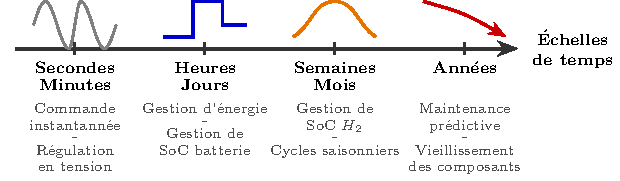
\includegraphics[width=0.8\linewidth]{Chapitre 2/Figures/timescales_fr.pdf}
    \caption{Échelles de temps opérationnelles du micro-réseau.}
    \label{fig:timescales}
\end{figure}
\FloatBarrier

Cette disparité temporelle constitue la difficulté centrale du problème et le fil conducteur de ce travail~: une EMS pertinente doit articuler des décisions immédiates (répartir la puissance maintenant) avec leurs conséquences à très long terme (l'usure cumulée des composants), sans négliger l'échelle intermédiaire des aléas.
La plupart des travaux de la littérature, comme la suite le montrera, ne traitent qu'une seule de ces strates à la fois.

Le parti pris méthodologique adopté ici consiste à séparer ces échelles et à fixer le niveau de travail de l'EMS.
Les couches de contrôle bas niveau (commande des convertisseurs, MPPT, régulation du bus) opèrent à l'échelle infra-seconde et sont supposées assurées par des contrôleurs locaux dédiés~; elles sortent du périmètre de cette étude.
L'EMS étudiée travaille à une résolution horaire~: assez fine pour capter les dynamiques journalières de la production et de la demande, mais assez grossière pour autoriser des simulations sur plusieurs décennies, indispensables pour observer le vieillissement et chiffrer les coûts de remplacement.
C'est à cette résolution qu'une même stratégie peut être évaluée à la fois sur le service rendu à court terme et sur la durabilité à long terme.
À chacune des trois strates correspond un critère de performance (fiabilité d'alimentation, durabilité, robustesse aux défaillances) dont la définition formelle fait l'objet de la section~\ref{sec:indicateurs}.

\subsection{Question de recherche}

Le cadre de travail et les définitions étant posés, et au regard de la segmentation de la littérature selon l'échelle de temps traitée, la question de recherche structurant ce chapitre peut être introduite~:

\begin{align*}
    \tcboxmath{
        \parbox{.93\textwidth}{
            \centering
            \textbf{\text{Quels critères permettent d'évaluer et de comparer objectivement des stratégies}}\\
            \textbf{\text{de gestion d'énergie pour un micro-réseau hybride isolé, en tenant compte}}\\
            \textbf{\text{simultanément des différentes échelles de temps mises en jeu, et quelle}}\\
            \textbf{\text{stratégie offre alors le meilleur compromis~?}}
        }
    }
\end{align*}

Pour y répondre, ce chapitre commence par dresser l'état de l'art des objectifs et des structures d'EMS (section~\ref{sec:eda}), avant de présenter le modèle du système et les profils de puissance retenus (section~\ref{sec:modele}).
Les trois indicateurs de performance qui serviront à juger les stratégies sont ensuite définis (section~\ref{sec:indicateurs}), avant que soient précisés l'usage réactif fait de l'information de SoH (section~\ref{sec:soh}) ainsi que le cadre d'évaluation et l'algorithme de simulation (section~\ref{sec:simulation}).
Les stratégies considérées et leurs performances dans le plan de Pareto sont alors analysées (sections~\ref{sec:ems}-\ref{sec:resultats}), avant d'éprouver leur robustesse aux défaillances (section~\ref{sec:robustesse}) et la sensibilité des résultats aux hypothèses de modélisation (section~\ref{sec:sensibilite}).
La section~\ref{sec:conclusion_chap} conclut le chapitre.

% ============================================================
%  CHAPITRE 2 — Section 1 : État de l'art
%  À intégrer dans le chapitre :
%  \chapter{Méthodologie pour les stratégies de gestion d'énergie
%           pour une approche réactive au vieillissement}
% ============================================================

\section{État de l'art}
\label{sec:eda}

Les stratégies de gestion d'énergie constituent le c\oe{}ur décisionnel des microréseaux hybrides.
Leur rôle est de déterminer, à chaque instant, comment répartir la puissance entre les différentes sources et les différents stockages afin de satisfaire la demande des utilisateurs, tout en respectant les contraintes physiques et opérationnelles du système.
La conception d'une EMS efficace nécessite de répondre à deux questions fondamentales~: quels objectifs optimiser, et quelle structure de contrôle adopter pour les atteindre.
Ces deux questions, qui structurent la littérature sur le sujet, sont abordées successivement dans les sous-sections qui suivent, avant de positionner les travaux présentés dans ce chapitre par rapport à l'état de l'art.

La gestion d'énergie des micro-réseaux, et en particulier de ceux couplant batteries et chaîne hydrogène, constitue un champ de recherche très actif, comme en témoignent plusieurs revues récentes~\cite{zhu_comprehensive_2026}\cite{esparza_review_2025}\cite{chowdhury_optimization_2026}.
Ces synthèses recensent une grande variété d'objectifs assignés aux EMS, regroupables en quelques grandes familles~: la fiabilité et la continuité de l'alimentation, la performance économique (coût d'exploitation, de carburant ou de remplacement), le rendement énergétique et la qualité de l'énergie fournie, et enfin la durabilité des composants et l'empreinte environnementale du système~\cite{esparza_review_2025}\cite{chowdhury_optimization_2026}.
Les objectifs poursuivis étant fortement dépendants de l'application considérée, les stratégies de gestion d'énergie sont généralement conçues comme un compromis entre plusieurs critères, souvent antagonistes. Les deux sous-sections suivantes présentent successivement les objectifs les plus fréquemment retenus dans la littérature, puis les principales structures d'EMS proposées pour les atteindre.

% ------------------------------------------------------------
\subsection{Objectifs des EMS}
% ------------------------------------------------------------

Les objectifs assignés aux EMS sont fondamentalement dictés par les constantes de temps des phénomènes ciblés.
Or, celles-ci s'étendent sur plusieurs ordres de grandeur~: de la milliseconde pour la stabilité de la tension du bus continu, à l'heure pour l'équilibre offre-demande, jusqu'à l'année, voire la décennie, pour les phénomènes de vieillissement des composants.
Cette disparité temporelle est à l'origine d'une segmentation de la littérature, dans laquelle les travaux traitent le plus souvent d'une seule échelle de temps, sans chercher à articuler les différentes dimensions du problème.

\subsubsection{Objectifs à court terme.}
Une première branche de la littérature se concentre sur la dynamique à court terme, avec pour objectif principal le maintien de la qualité de service et la stabilité du réseau.
Hu \textit{et al.} proposent ainsi un contrôle sans modèle pour un système autonome photovoltaïque équipé d'un stockage hybride batterie-supercondensateur~: ne s'appuyant que sur les données d'entrée-sortie du système, leur stratégie lisse les fluctuations de puissance tout en maintenant stable la tension du bus continu, sur une échelle de temps allant de la seconde à la minute~\cite{hu_data_based_2024}.
Dans le même esprit, Asrari \textit{et al.} valident expérimentalement, sur un micro-réseau de laboratoire, un contrôleur de charge programmable couplé à un stockage hybride batterie-supercondensateur et à un suivi du point de puissance maximale (MPPT)~: par rapport à un contrôleur figé, il réduit les fluctuations de courant et le taux de distorsion harmonique d'environ deux tiers, le supercondensateur déchargeant la batterie des transitoires rapides et prolongeant ainsi sa durée de vie~\cite{asrari_experimental_2025}.
Si ces approches sont efficaces pour l'équilibrage instantané et la qualité de l'énergie, elles reposent sur des limitations de courant heuristiques et ne tiennent pas compte des mécanismes de dégradation à long terme ni des contraintes opérationnelles s'étendant sur des heures ou des jours.

\subsubsection{Objectifs à moyen terme.}
À une échelle intermédiaire, les travaux se tournent vers l'optimisation économique, l'écrêtage des pics de charge et la coordination sur quelques heures à quelques jours.
Paulraj \textit{et al.} entraînent un réseau de neurones récurrent de type LSTM pour générer en temps réel la consigne de courant d'un supercondensateur épaulant la batterie d'un véhicule électrique~: sur des cycles de conduite normalisés, le courant de crête de la batterie est réduit de 21 à 33~\%, la puissance de pointe appelée d'environ 30~\% et la consommation énergétique de 6 à 12~\%, allégeant d'autant la sollicitation de la batterie~\cite{paulraj_machine_2025}.
Cette approche reste toutefois cantonnée à une seule constante de temps et ne rend pas compte du vieillissement cumulé sur des périodes plus longues.
Dans le contexte des micro-réseaux à hydrogène, Guo \textit{et al.} proposent une commande prédictive économique hiérarchique à deux niveaux~: le niveau supérieur, résolu sur un horizon long, planifie les cycles de démarrage-arrêt de l'électrolyseur et de la pile à combustible ainsi que la trajectoire de SoC de la batterie, tandis que le niveau inférieur réoptimise à court terme le suivi de la demande de puissance, en alignant le fonctionnement sur les prévisions météorologiques et les signaux de marché~\cite{guo_sustainable_2025}.
Bien que ce cadre relie les échelles horaire et hebdomadaire, il n'intègre pas explicitement la dégradation physique des composants au-delà de l'horizon de planification.

\subsubsection{Objectifs à long terme.}
Une troisième branche s'attache aux objectifs de long terme, tels que le transfert saisonnier d'énergie ou la préservation des composants sur plusieurs années.
Qi \textit{et al.} proposent un cadre d'optimisation coordonnée à deux étages, sans recours à la prévision~: une trajectoire annuelle de référence du stockage hydrogène est calculée hors ligne, puis réactualisée en ligne par régression à noyau et suivie au moyen d'un algorithme d'optimisation convexe en ligne à file d'attente virtuelle~\cite{qi_long_term_2025}.
Sur des jeux de données réels, ce cadre réduit le coût d'exploitation et la défaillance de charge d'environ 60 et 90~\% respectivement par rapport à une commande prédictive, mais il ne représente pas la détérioration physique des organes de stockage.
À l'opposé, Wang \textit{et al.} placent précisément la dégradation au c\oe{}ur de l'objectif~: leur stratégie de gestion de puissance pour un véhicule hybride pile à combustible-batterie intègre un modèle électrochimique simplifié de perte de surface active de la pile (sous l'effet des transitoires, des démarrages-arrêts, du ralenti et des fortes puissances) ainsi qu'un modèle empirique de perte de capacité de la batterie en fonction du régime de courant~\cite{wang_power_2019}.
L'inclusion de ces termes de dégradation dans la fonction de coût prolonge la durée de vie de la pile, au prix d'un vieillissement accru de la batterie, pour un coût total d'usage moindre sur la durée de vie.
Leur modèle suppose néanmoins que le suivi de charge à court terme, fixé ici par le cycle de conduite, est déjà assuré, écartant de fait les fluctuations de puissance en temps réel.

Ce panorama, résumé dans le Tableau~\ref{tab:state_of_art_summary}, met en évidence un manque persistant dans la littérature~: celui d'un cadre méthodologique qui couple explicitement la fiabilité d'alimentation à court terme avec une gestion active et consciente de la santé des composants de stockage sur le long terme.

\begin{table}[h!]
\centering
\caption{État de l'art des objectifs des EMS et constantes de temps associées.}
\label{tab:state_of_art_summary}
\begin{tabularx}{\textwidth}{lXX}
\hline
\textbf{Réf.} & \textbf{Contribution} & \textbf{Lacune identifiée} \\ \hline
\cite{hu_data_based_2024} & Suivi de charge en temps réel et stabilité du bus continu (secondes à minutes). & Pas de vieillissement à long terme, pas de dynamique au-delà de la minute. \\ \hline
\cite{asrari_experimental_2025} & Amélioration de la qualité de l'énergie et suivi solaire avec limitations de courant heuristiques. & Limitée à une seule constante de temps court terme, pas de boucle sur le vieillissement. \\ \hline
\cite{paulraj_machine_2025} & Optimisation du courant de crête de la batterie et de la consommation énergétique (secondes à heures). & Pas de suivi de santé à long terme ; unique constante de temps intermédiaire. \\ \hline
\cite{guo_sustainable_2025} & MPC économique hiérarchique pour la gestion de l'hydrogène et l'intégration marché/météo. & N'intègre pas explicitement la dégradation physique ni le vieillissement à long terme. \\ \hline
\cite{qi_long_term_2025} & Coordination du transfert saisonnier d'énergie et de l'intermittence renouvelable sur le long terme. & Ne prend pas en compte la détérioration physique des composants. \\ \hline
\cite{wang_power_2019} & Réduction de la dégradation électrochimique des PAC et batteries sur plusieurs années. & Suppose que les fluctuations de puissance à court terme sont déjà gérées par une couche externe. \\ \hline
\end{tabularx}
\end{table}
\FloatBarrier

% ------------------------------------------------------------
\subsection{Structures des EMS}
% ------------------------------------------------------------

Au-delà des objectifs poursuivis, la conception d'une EMS requiert le choix d'une structure de contrôle adaptée.
Les approches publiées dans la littérature peuvent être regroupées en trois grandes familles~: (i) les stratégies à base de règles (\textit{rule-based}), (ii) les stratégies à base d'optimisation (\textit{optimization-based}), et (iii) les méthodes pilotées par les données (\textit{data-driven}).
L'accent est ici mis sur les EMS en ligne, compatibles avec une implémentation en temps réel dans un microréseau réel.

\subsubsection{Stratégies à base d'optimisation.}
Les approches par optimisation reposent le plus souvent sur la commande prédictive (\textit{Model Predictive Control}, MPC), qui détermine les consignes en résolvant à chaque pas un problème d'optimisation sous contraintes sur un horizon glissant.
K/bidi \textit{et al.} développent ainsi une stratégie multi-étages pour un micro-réseau photovoltaïque doté d'une batterie, d'une pile à combustible et d'un électrolyseur~: une commande prédictive explicite distribuée assure la gestion de puissance (PMS) tandis qu'une programmation quadratique mixte en nombres entiers résout le problème d'engagement des unités au niveau de la gestion d'énergie (EMS), l'étude portant une attention particulière à l'interaction, souvent négligée, entre ces deux couches afin d'éviter les démarrages intempestifs de la pile et de l'électrolyseur~\cite{kbidi_multistage_2022}.
Hou \textit{et al.} proposent quant à eux une MPC hiérarchique multi-horizon pour véhicule à pile à combustible~: une couche supérieure planifie sur horizon long la trajectoire de référence du SoC de la batterie, et une couche inférieure réalise l'optimisation temps réel (consommation d'hydrogène, durée de vie des composants, suivi du SoC)~; une paramétrisation des variables de commande réduit le temps de calcul, pour un gain de coût de 4 à 5~\% et une efficacité de calcul améliorée de près de 20~\% par rapport à une MPC classique, validés sur banc \textit{hardware-in-the-loop}~\cite{hou_hierarchical_2025}.
Si ces méthodes atteignent une efficacité théorique élevée, leurs performances restent tributaires de la qualité des prévisions et exigent une puissance de calcul significative pour une exécution en ligne.

\subsubsection{Méthodes pilotées par les données.}
Les méthodes pilotées par les données, et au premier chef l'apprentissage par renforcement (\textit{Reinforcement Learning}, RL), apprennent une politique de contrôle par interaction répétée avec un modèle du système, sans formulation explicite du problème d'optimisation.
Han \textit{et al.} montrent qu'une stratégie de \textit{Double Deep Q-Learning}, dans laquelle la vitesse de variation de puissance de la pile est introduite comme variable d'action, améliore l'économie de carburant d'un autobus à pile à combustible de l'ordre de 15~\% par rapport à des règles standards, y compris sur des scénarios non rencontrés à l'entraînement~\cite{han_reinforcement_2025}.
Pour pallier les limites de stabilité et de généralisation des approches purement apprises, des structures hybrides combinent apprentissage et méthodes classiques.
Ren \textit{et al.} couplent un réseau de neurones de prédiction de la demande à une stratégie de minimisation de la consommation équivalente (ECMS), dont un agent d'apprentissage profond ajuste les paramètres pour préserver la batterie, réduisant le débit de charge cumulé d'environ 3~\% à consommation maîtrisée~\cite{ren_battery_2024}.
Dans le même esprit, Liu \textit{et al.} associent une MPC (garante de la stabilité et du respect des contraintes) à une politique d'apprentissage venant la compenser pour les décisions de long terme~: leur stratégie réduit la dégradation de la pile à combustible de plus de 50~\% au prix d'un léger surcroît de dégradation de la batterie, pour le coût d'exploitation le plus faible des méthodes comparées~\cite{liu_novel_2025}.
Ces approches sont prometteuses mais restent gourmandes en données d'entraînement et offrent peu de garanties de comportement hors du domaine appris.

\subsubsection{Stratégies à base de règles.}
Malgré les gains rapportés par les méthodes prédictives et apprises, les stratégies à base de règles demeurent la référence des applications industrielles, par leur transparence et leur faible coût de calcul.
Le principe en est direct~: la décision de répartition découle de l'état courant du système (signe du bilan de puissance, niveau de SoC, etc.) au travers de seuils et de lois explicites, sans résolution d'un problème d'optimisation ni modèle de prévision.
Les déclinaisons en sont nombreuses.
Nivolianiti \textit{et al.} recourent à la logique floue pour répartir la puissance dans un navire à propulsion hydrogène et montrent qu'elle réduit la consommation de carburant mieux que des approches déterministes ou par optimisation, sans nécessiter d'information sur l'avenir~\cite{nivolianiti_fuzzy_2024}.
Une variante très répandue pilote la répartition par le SoC de la batterie au travers de règles par morceaux, réservant les composants lents (hydrogène) aux régimes extrêmes de charge et confiant la dynamique rapide à la batterie~\cite{koltermann_improved_2024}\cite{yuan_real-time_2022}~: Koltermann \textit{et al.} valident ainsi, sur un système de 6~MW, un algorithme fixant des objectifs de SoC, de débit et de puissance qui lissent les commutations et portent le rendement à environ 82~\%, tandis que Yuan \textit{et al.} calibrent par algorithme génétique les seuils de charge-décharge selon le profil d'usage.
Une autre famille fait fonctionner la chaîne hydrogène à puissance sensiblement constante, la batterie absorbant le résidu rapide~\cite{wang_comparison_2020}.
À ces logiques se rattachent les stratégies de répartition statique de puissance (\textit{power splitting}) ou de séparation fréquentielle (\textit{frequency splitting}), où batterie et hydrogène se partagent respectivement les composantes rapides et lentes de la sollicitation~\cite{eldeeb_hybrid_2019}\cite{corapsiz_overview_2023}.
Ces logiques, dont plusieurs sont reprises comme stratégies de référence dans ce chapitre, sont à la fois simples à implémenter et lisibles pour un opérateur.

L'intérêt des règles ne tient pas qu'à leur simplicité.
Wang \textit{et al.} comparent une gestion à base de règles et une MPC pour un véhicule hybride pile à combustible-batterie en intégrant la dégradation des deux composants~: de façon contre-intuitive, la stratégie à base de règles atteint un coût total d'usage inférieur sur la durée de vie, alors même que la MPC dispose d'une connaissance anticipée du cycle~; ce résultat s'explique par l'évolution des poids relatifs des facteurs de coût au fil du vieillissement~\cite{wang_comparison_2020}.
Dans le même sens, Wu \textit{et al.} comparent des stratégies purement à base de règles, par optimisation et hybrides, et concluent que si l'hybridation améliore l'efficacité, les fondations à base de règles offrent la robustesse opérationnelle la plus élevée, notamment en limitant les cycles de démarrage-arrêt de la pile~\cite{wu_rule_2023}.
C'est cette robustesse, alliée au déterminisme et au faible coût de calcul indispensable aux simulations pluriannuelles, qui motive le choix de cette famille dans le présent travail.
Le prix à payer est une optimalité théorique moindre que celle des méthodes prédictives~; une conception soignée des règles, complétée par l'exploitation réactive de l'information de vieillissement, permet toutefois d'atteindre des compromis très satisfaisants.

% ------------------------------------------------------------
\subsection{Positionnement de l'étude}
% ------------------------------------------------------------

Au regard des travaux recensés, une lacune commune se dégage.
La plupart des cadres de gestion d'énergie existants privilégient soit l'efficacité opérationnelle à court terme (minimisation du coût instantané, de la consommation ou de la demande non satisfaite), soit la préservation des composants à long terme au travers de termes de coût de dégradation.
Rares sont les approches traitant ces deux dimensions simultanément, alors même que les phénomènes sous-jacents évoluent sur des échelles de temps fondamentalement différentes~: l'équilibre de puissance et la continuité de service relèvent de la seconde à la minute, tandis que la dégradation des composants se joue sur des mois, voire des années.
Une troisième échelle, intermédiaire, est plus rarement encore prise en compte~: celle des aléas d'exploitation (défaillance temporaire d'un composant, puis reprise du service), à laquelle se rattache la robustesse de la stratégie. Les travaux présentés dans ce chapitre s'inscrivent dans cette problématique, et la contribution centrale réside dans un cadre d'évaluation capable de juger une même stratégie de gestion d'énergie sur ces trois échelles de temps à la fois. La fiabilité et la durabilité sont quantifiées par deux indicateurs définis en régime nominal, qui permettent de représenter et de comparer les stratégies dans un plan de Pareto~; la robustesse est appréciée séparément, à travers le comportement des stratégies en situation de panne.

Deux éléments de ce chapitre complètent ce cadre.
D'une part, l'information de SoH issue du diagnostic du chapitre précédent est exploitée de manière réactive, afin de maintenir les composants à l'intérieur de leurs plages de fonctionnement, lesquelles se réduisent avec l'âge~; cette approche réactive, commune à toutes les stratégies comparées, se distingue de l'usage anticipatif développé au chapitre suivant.
D'autre part, la généralité des conclusions est éprouvée par une analyse de sensibilité aux principales hypothèses de modélisation.
Les stratégies comparées ne sont, quant à elles, pas individuellement nouvelles~: chacune est une déclinaison représentative d'une logique de contrôle à base de règles présente dans la littérature, et leur intérêt tient à leur comparaison unifiée au sein du cadre proposé.


% ============================================================
%  CHAPITRE 2 — Section : Modélisation du système
% ============================================================

\section{Modélisation du système}
\label{sec:modele}

L'évaluation des stratégies de gestion d'énergie requiert au préalable un modèle du système suffisamment fidèle pour reproduire les flux de puissance et l'évolution des organes de stockage, mais suffisamment léger pour être simulé sur plusieurs décennies. Cette section précise le modèle macroscopique retenu~: les équations d'évolution de l'état du système d'une part, les profils de puissance qui en constituent les sollicitations d'autre part. L'architecture du micro-réseau a été présentée au chapitre précédent et n'est pas reprise ici~: champ photovoltaïque, batterie lithium-ion et chaîne hydrogène (pile à combustible et électrolyseur) interconnectés autour d'un bus continu commun, en site isolé à La Réunion. Son dimensionnement nominal est simplement rappelé au Tableau~\ref{tab:system_parameters} (section~\ref{sec:ems}).

% ------------------------------------------------------------
\subsection{Équations d'évolution de l'état du système}
\label{subsec:eqs_evolution}
% ------------------------------------------------------------

L'état du système est décrit par deux grandeurs~: l'état de charge $\mathrm{SoC}$ de la batterie et l'énergie $E_{\text{H2}}$ [J] stockée sous forme d'hydrogène. Entre les instants $t$ et $t+\Delta t$, leurs évolutions sont régies par les bilans suivants~:
\begin{equation}
    \label{eq:soc_evol_sys}
    \mathrm{SoC}(t+\Delta t) = \mathrm{SoC}(t) - \frac{P_{\text{bat}}(t)\,\Delta t}{E_{\text{bat,nom}}}\,\eta_{\text{bat}}^{\,k}
\end{equation}
\begin{equation}
    \label{eq:eh2_evol_sys}
    E_{\text{H2}}(t+\Delta t) = E_{\text{H2}}(t) - \Big( P_{\text{ELY}}(t)\,\eta_{\text{ELY}}(t) + \frac{P_{\text{FC}}(t)}{\eta_{\text{FC}}(t)} \Big)\,\Delta t
\end{equation}
où $P_{\text{bat}}$ [W] est la puissance de la batterie, comptée positive en décharge, $E_{\text{bat,nom}}$ [J] son énergie nominale, et $\eta_{\text{bat}}^{\,k}$ son rendement, avec $k=1$ en charge et $k=-1$ en décharge. Ce rendement est ici supposé constant et égal à $0{,}95$. Du côté hydrogène, $P_{\text{ELY}}$ [W] est la puissance de l'électrolyseur, négative par nature puisqu'il ne peut que consommer, et $P_{\text{FC}}$ [W] celle de la pile à combustible, positive par nature puisqu'elle ne peut que produire~; $\eta_{\text{ELY}}$ et $\eta_{\text{FC}}$ sont leurs rendements respectifs, qui dépendent du point de fonctionnement~\cite{lu_optimization_2023}\cite{jia_novel_2023}.

Ces rendements sont implémentés sous forme de tables de correspondance exprimant le rendement de conversion en fonction de la puissance relative de fonctionnement. Ce choix présente un intérêt particulier au regard du vieillissement~: lorsqu'un composant vieillit, sa puissance maximale délivrable diminue, de sorte que fournir une même puissance absolue correspond à une charge \emph{relative} plus élevée, et donc à un point différent le long de la courbe de rendement. La perte d'efficacité associée au vieillissement est ainsi capturée implicitement par ce déplacement du point de fonctionnement dans la table, qui se traduit par une consommation d'hydrogène accrue à service équivalent à mesure que les composants se dégradent.

À tout instant, le bilan de puissance sur le bus continu assure la conservation de l'énergie~:
\begin{equation}
    \label{eq:power_balance_sys}
    P_{\text{Load}} - P_{\text{PV}} = P_{\text{FC}} + P_{\text{ELY}} + P_{\text{bat}}
\end{equation}
où $P_{\text{Load}}$ [W] est la puissance consommée par les usagers (positive) et $P_{\text{PV}}$ [W] la puissance fournie par les panneaux (positive). Ces deux valeurs peuvent différer des trajectoires planifiées $\hat{P}_{\text{Load}}$ et $\hat{P}_{\text{PV}}$ issues des profils~: un tel écart apparaît, par exemple, lorsque la demande ne peut être satisfaite par les composants ou lorsqu'un écrêtage est réalisé.

Dans cette formulation, les variables de contrôle du système sont les trois puissances $P_{\text{bat}}$, $P_{\text{FC}}$ et $P_{\text{ELY}}$~; il s'agit donc d'un problème de commande à trois dimensions. Une fois ces trois puissances déterminées par l'EMS, le bilan global~\eqref{eq:power_balance_sys} est évalué et peut, le cas échéant, s'écarter de la trajectoire de référence~: cette latitude permet au système de \emph{ne pas} suivre exactement la demande à certains instants lorsque la réduction de la dégradation est jugée prioritaire. Les contraintes opérationnelles (puissances maximales des composants, bornes de SoC, capacité du réservoir d'hydrogène) sont respectées lors de cette allocation, comme détaillé dans l'algorithme de simulation (section~\ref{sec:simulation}).

% ------------------------------------------------------------
\subsection{Profils de puissance}
\label{subsec:profils}
% ------------------------------------------------------------

Les sollicitations du système sont entièrement déterminées par deux profils temporels~: la production photovoltaïque $\hat{P}_{\text{PV}}$ et la demande de charge $\hat{P}_{\text{Load}}$. Ces profils ne sont pas synthétiques~: ils proviennent de données de terrain fournies par le concepteur du micro-réseau à La Réunion. Aucun modèle de conversion irradiance-puissance (inclinaison des panneaux, conversion du rayonnement global horizontal, etc.) n'intervient donc~: le profil PV est directement issu de mesures de production sur site, tandis que le profil de charge résulte d'enquêtes de terrain sur les habitudes de consommation des résidents locaux, agrégées pour constituer un profil de consommation représentatif (Figure~\ref{fig:profiles}).

\begin{figure}[h!]
    \centering
    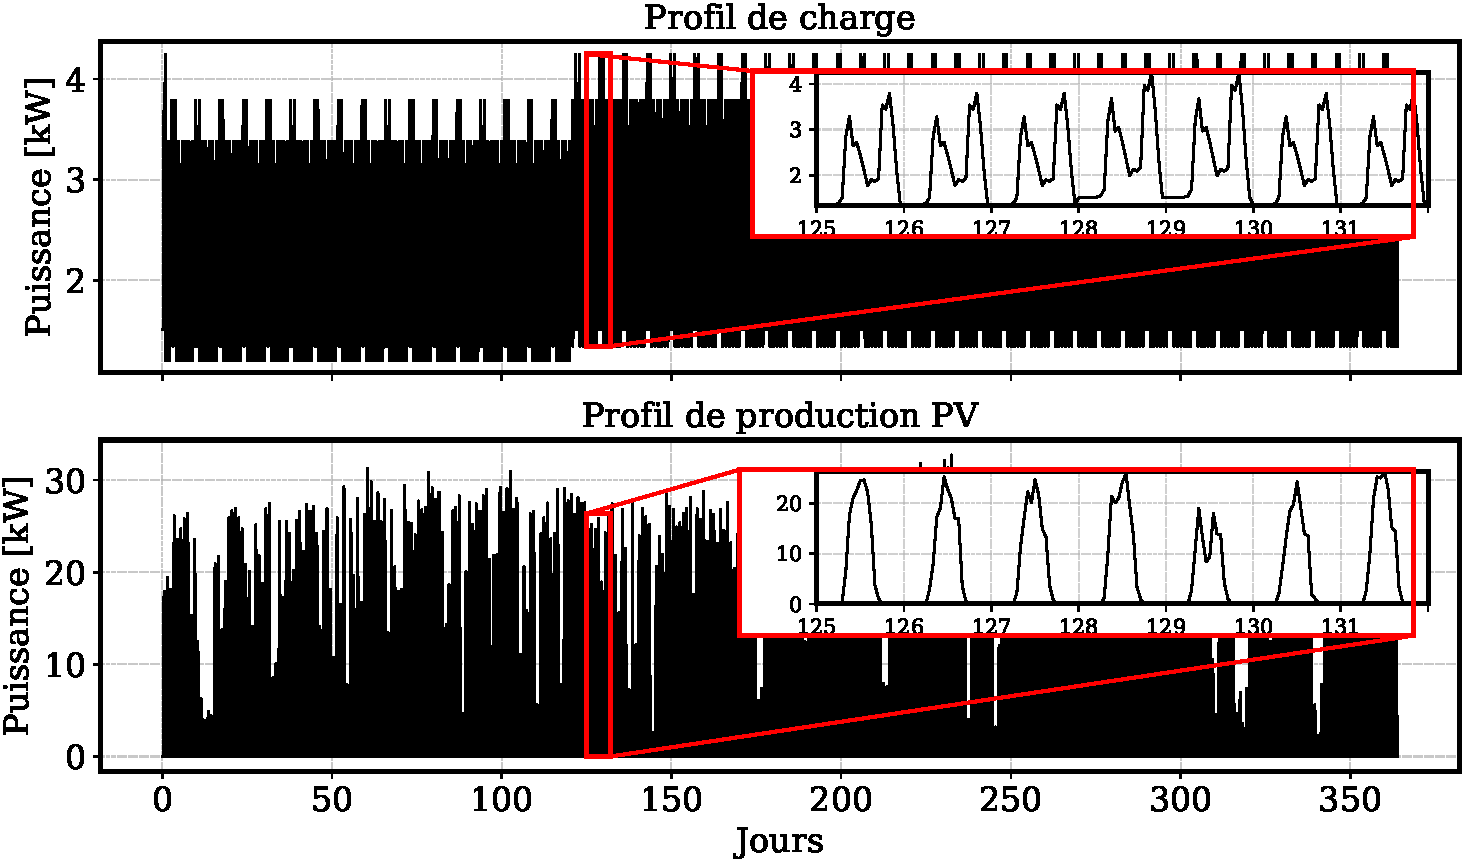
\includegraphics[width=\linewidth]{Chapitre 2/Modele/Figures/sidelec_conso_PV_fr.pdf}
    \caption{Profils de puissance utilisés en simulation~: charge et production photovoltaïque }
    \label{fig:profiles}
\end{figure}
\FloatBarrier

Deux caractéristiques de ces profils méritent d'être soulignées, car elles conditionnent l'interprétation des résultats. D'une part, la production PV est nettement surdimensionnée relativement à la demande moyenne~: la puissance crête du champ (environ \SI{33}{\kilo\watt}) dépasse largement la charge moyenne (de l'ordre de \SI{2}{\kilo\watt}), ce qui se traduit par d'importants excédents d'énergie en journée, dont l'électrolyseur et la batterie doivent disposer, ou par un niveau important d'écrêtage. D'autre part, en raison de la position quasi équatoriale de l'île, la variabilité \emph{saisonnière} de la ressource solaire comme de la demande est relativement limitée~; les profils mesurés intègrent néanmoins la variabilité réelle, jour après jour et à l'intérieur de chaque journée, de la production et de la consommation du site. Ce contexte (fort excédent PV, faible saisonnalité) est caractéristique du cas d'étude et devra être gardé à l'esprit lors de la généralisation des conclusions à d'autres sites (cf.\ section~\ref{sec:conclusion_chap}).

% ============================================================
%  CHAPITRE 2 — Section 2 : Définition des indicateurs de performance
% ============================================================

\section{Définition des indicateurs de performance}
\label{sec:indicateurs}

Afin d'évaluer et de comparer les différentes EMS dans le cadre proposé, il est nécessaire de disposer d'indicateurs de performance bien définis, capables de rendre compte de la qualité du service rendu aux utilisateurs, de l'impact de la stratégie sur la durée de vie des composants, et de la résilience du système face aux aléas. Ces trois dimensions correspondent respectivement aux objectifs de court, long et moyen terme introduits dans la section précédente, et elles évoluent sur des échelles de temps fondamentalement différentes. Trois indicateurs complémentaires sont donc introduits~: la probabilité de coupure d'alimentation (LPSP), qui quantifie la fiabilité à court terme~; un coût de dégradation agrégé, qui chiffre l'usure à long terme induite par les décisions de contrôle~; et un indicateur de robustesse, qui mesure le service maintenu (au sens de la LPSP) lors d'une défaillance temporaire de composant. Les deux premiers indicateurs sont définis ci-dessous puis exploités dans le plan de Pareto tout au long du chapitre~; le troisième, dont la définition et le protocole d'évaluation sont établis ici, est mis en œuvre à la section~\ref{sec:robustesse}.

% ------------------------------------------------------------
\subsection{LPSP}
% ------------------------------------------------------------

Dans le contexte de cette étude, la qualité du service est évaluée strictement du point de vue de la continuité d'alimentation du consommateur. L'attention est donc portée sur le déficit de puissance. Les situations de surplus énergétique, dans lesquelles la production renouvelable excède à la fois la demande de charge et la capacité de charge des systèmes de stockage, communément appelées écrêtage (\textit{curtailment}), ne sont pas directement pénalisées par cet indicateur. Il est supposé que, durant ces intervalles, la stratégie de contrôle adapte l'algorithme de suivi du point de puissance maximale (MPPT) afin d'écrêter la production solaire, maintenant ainsi la stabilité du bus continu sans affecter la fourniture d'énergie à la charge.

L'indicateur retenu pour quantifier la fiabilité est la \textit{Loss of Power Supply Probability} (LPSP). Cette métrique est largement adoptée dans la littérature traitant de la gestion d'énergie et du dimensionnement des systèmes d'énergie renouvelable hybrides~\cite{korovushkin_modern_2025}\cite{heydari_combined_2023}. La LPSP est définie comme la fraction de la demande totale en énergie qui ne peut pas être satisfaite par le système hybride sur un horizon de temps donné. Elle varie entre 0 et 1~: une valeur de 0 signifie que la charge est intégralement satisfaite à tout instant, tandis qu'une valeur de 1 correspond à une charge jamais satisfaite. Mathématiquement, la LPSP s'exprime comme le rapport entre le déficit énergétique cumulé et la demande énergétique totale sur l'ensemble de la période de simulation~:

\begin{equation}
    \mathrm{LPSP} = \frac{\sum_{t} \mathrm{LPS}(t)\cdot \Delta t}{\sum_{t} \hat{P}_{\text{Load}}(t) \cdot \Delta t}
    \label{eq:lpsp}
\end{equation}

où $\mathrm{LPS}(t)$ [W] représente la perte de puissance d'alimentation à l'instant $t$, définie comme~:

\begin{equation}
    \mathrm{LPS}(t) =
    \begin{cases}
      \hat{P}_{\text{Load}}(t) - P_{\text{Avail}}(t) & \text{si } \hat{P}_{\text{Load}}(t) > P_{\text{Avail}}(t) \\
      0 & \text{sinon}
    \end{cases}
    \label{eq:lps}
\end{equation}

où $\hat{P}_{\text{Load}}(t)$ [W] est la puissance demandée par la charge à l'instant $t$, et $P_{\text{Avail}}(t)$ [W] est la puissance totale disponible auprès de la production PV et des systèmes de stockage à cet instant.

% ------------------------------------------------------------
\subsection{Robustesse face aux défaillances}
\label{subsec:indic_robustesse}
% ------------------------------------------------------------

La LPSP rend compte de la qualité du service en régime nominal, lorsque tous les composants sont opérationnels. Un micro-réseau isolé est toutefois, par construction, dépourvu de secours extérieur~: la défaillance temporaire d'un organe de stockage (défaut d'un module hydrogène, déclenchement d'une protection, opération de maintenance...) peut survenir en cours d'exploitation et compromettre la continuité de service. Cette dimension relève d'une échelle de temps intermédiaire, entre la dynamique horaire du suivi de charge et la dynamique pluriannuelle du vieillissement~: une panne dure typiquement de quelques heures à quelques jours, le temps de la réparation. Un tel régime dégradé n'est rendu par aucun des indicateurs de fonctionnement nominal, ni la fiabilité ni la durabilité, et appelle donc une métrique propre.

Les défaillances considérées ici ne portent que sur les composants hydrogène (PEMFC et PEMWE). Les données de fiabilité de terrain (\textit{Mean Time Between Failure (MTBF), Mean Time To Failure (MTTF)...}) restent rares et difficiles à unifier, les trois technologies ne se prêtant à aucun référentiel commun, mais leur triangulation à partir de sources disponibles (relevés de terrain pour la batterie~\cite{ieee_std_493_2007}, feuilles de route technico-économiques pour la pile à combustible~\cite{fch2ju_mawp_2018}, analyse par arbre de défaillances pour l'électrolyseur~\cite{ubale_failure_2025}) fait apparaître un écart de deux à trois ordres de grandeur~: les défaillances de la batterie sont beaucoup plus rares que celles des composants hydrogène. Il est donc cohérent de concentrer l'analyse sur ces derniers, la batterie jouant alors le rôle de réserve de repli.

Une défaillance est modélisée comme l'indisponibilité temporaire d'un composant hydrogène, survenant à un instant $t_0$ et réparée au bout d'une semaine ($\Delta t_{\text{panne}} = \SI{168}{\hour}$). Deux sévérités sont retenues~: la défaillance totale (puissance du composant ramenée à \SI{0}{\percent}) et la défaillance partielle (puissance maximale dégradée à \SI{50}{\percent}). Les piles à combustible et les électrolyseurs PEM sont des assemblages modulaires, si bien qu'un défaut localisé (cellule défaillante, \textit{stack} isolé par sa protection, auxiliaire de \textit{balance-of-plant} défaillant...) met hors service une fraction du composant sans l'arrêter complètement. Une perte de l'ordre de la moitié de la capacité constitue ainsi un mode de défaillance représentatif, et éprouve la capacité de l'EMS à exploiter la puissance résiduelle. Croisées avec les deux composants, ces sévérités définissent quatre scénarios~: PEMFC totale, PEMFC \SI{50}{\percent}, PEMWE totale et PEMWE \SI{50}{\percent}.

L'indicateur de robustesse est la LPSP subie en présence de la panne, mesurée sur une fenêtre d'évaluation $[t_0,\, t_0 + \Delta t_{\text{éval}}]$. Les dégradations des composants ne sont pas prioritaires dans ce cas puisqu'il est considéré que l'acheminement de puissance pour assurer le service aux usagers sur cette courte période est l'aspect central. Pour un scénario $\sigma = (c, \kappa)$, défini par le composant défaillant $c \in \{\text{PEMFC}, \text{PEMWE}\}$ et un facteur de sévérité $\kappa \in \{0\,;\,0{,}5\}$, la puissance maximale du composant $c$ est plafonnée à $\kappa\, P_{\text{max}}^{c}$ pendant la panne, puis rétablie à $P_{\text{max}}^{c}$ après réparation. Il en résulte une puissance disponible $P_{\text{Avail}}^{\sigma}(t)$, et donc une perte d'alimentation $\mathrm{LPS}^{\sigma}(t)$ au sens de l'équation~\eqref{eq:lps}. La LPSP sous défaillance s'écrit alors~:
\begin{equation}
    \mathrm{LPSP}_{\text{panne}}^{\sigma}(t_0) = \frac{\displaystyle\sum_{t=t_0}^{t_0+\Delta t_{\text{éval}}} \mathrm{LPS}^{\sigma}(t)\cdot \Delta t}{\displaystyle\sum_{t=t_0}^{t_0+\Delta t_{\text{éval}}} \hat{P}_{\text{Load}}(t)\cdot \Delta t}
    \label{eq:lpsp_panne}
\end{equation}
La fenêtre d'évaluation est volontairement plus longue que la panne~: $\Delta t_{\text{éval}} = 4\,\text{semaines}$, soit la semaine de défaillance suivie de trois semaines de reprise post-réparation. Cet allongement est nécessaire pour capturer le coût différé des pannes d'électrolyseur~: pendant l'indisponibilité du PEMWE, le surplus PV non électrolysé recharge la batterie et masque temporairement le déficit~; le vrai coût, un réservoir d'hydrogène appauvri et donc une pile à combustible en sous-alimentation, n'apparaît qu'après la réparation.

L'instant de panne $t_0$ étant a priori inconnu, il est traité comme une variable aléatoire de loi uniforme sur la période d'exploitation. L'indicateur de robustesse d'une stratégie $s$ pour le scénario $\sigma$ est alors défini comme l'espérance de la LPSP subie sous défaillance, estimée par la moyenne empirique sur $N$ instants de panne $t_0^{(n)}$~:
\begin{equation}
    R^{\sigma}(s) = \mathbb{E}_{t_0}\!\big[\mathrm{LPSP}_{\text{panne}}^{\sigma}(t_0)\big] \;\approx\; \frac{1}{N}\sum_{n=1}^{N} \mathrm{LPSP}_{\text{panne}}^{\sigma}\!\big(t_0^{(n)}\big),
    \label{eq:indic_robustesse}
\end{equation}
une stratégie étant d'autant plus robuste que $R^{\sigma}(s)$ est faible. À titre de diagnostic complémentaire, le surcoût de robustesse peut être rapporté~; il mesure l'écart à la LPSP qu'aurait connue la même stratégie sur la même fenêtre en l'absence de panne~:
\begin{equation}
    \Delta \mathrm{LPSP}_{\text{rob}}(t_0) = \mathrm{LPSP}_{\text{panne}}^{\sigma}(t_0) - \mathrm{LPSP}_{\text{nominal}}(t_0),
    \label{eq:surcout_robustesse}
\end{equation}
qui isole l'effet propre de la défaillance de la variabilité du profil de charge.

L'estimation de cette espérance repose sur une expérience de Monte-Carlo conçue pour isoler le comportement propre de chaque stratégie face à une panne, toutes choses égales par ailleurs. Une trajectoire de fond commune est d'abord établie en simulant sur deux ans la stratégie de référence RB2 (section~\ref{sec:resultats}), afin d'atteindre un régime permanent réaliste. Cette trajectoire fournit, à chaque heure, un instantané complet de l'état du système~: SoC de la batterie, niveau du réservoir d'hydrogène $E_{\text{H2}}$, états de santé et de vieillissement des composants. Le premier mois (environ 730~h) sert à établir ce régime permanent et est exclu des instants de panne, si bien que les instants $t_0^{(n)}$ sont tirés dans les mois 2 à 24. Partir d'une même trajectoire de fond garantit que toutes les stratégies sont éprouvées depuis un même état initial, ce qui rend la comparaison équitable.

À l'instant $t_0$, la simulation repart de cet instantané et déroule la fenêtre d'évaluation, le vieillissement étant gelé car négligeable à l'échelle de quelques semaines. La panne est supposée détectée par l'EMS~: à chaque pas, la stratégie évaluée calcule son intention de répartition normale, puis la puissance du composant défaillant est plafonnée à sa capacité disponible $\kappa\,P_{\text{max}}^{c}$ et le manque est rerouté vers la batterie. Les contraintes physiques du modèle, qui gèrent la saturation du SoC et du réservoir d'hydrogène, fixent enfin la puissance effectivement servie.

Le nombre de tirages est fixé à $N = 200$, les instants étant identiques pour toutes les stratégies et tous les scénarios, de sorte que la comparaison soit appariée et non polluée par le bruit d'échantillonnage. Ce protocole est résumé à la Figure~\ref{fig:rob_methodo}. Les stratégies ainsi évaluées sont les neuf EMS comparées dans ce chapitre (section~\ref{sec:ems})~; leurs résultats de robustesse sont analysés à la section~\ref{sec:robustesse}.

\begin{figure}[h!]
    \centering
    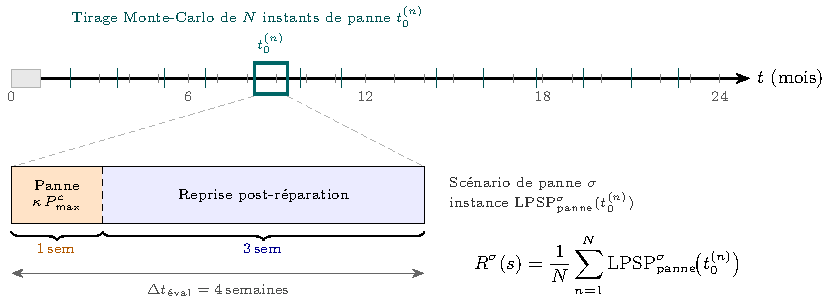
\includegraphics[width=\linewidth]{Chapitre 2/Robustesse/Figures/protocole_robustesse.pdf}
    \caption{Protocole d'évaluation de la robustesse par tirage Monte-Carlo des instants de panne.}
    \label{fig:rob_methodo}
\end{figure}
\FloatBarrier

% ------------------------------------------------------------
\subsection{Dégradations}
% ------------------------------------------------------------

Si la LPSP rend compte de l'adéquation à court terme du système, la performance à long terme est associée au taux de dégradation des principaux composants de stockage et de conversion. Ceux-ci sont soumis à des mécanismes d'usure directement liés aux décisions de l'EMS~: les cycles de charge et décharge de la batterie, les cycles de démarrage-arrêt des équipements hydrogène, les transients de puissance, ou encore les périodes de fonctionnement à forte charge. L'enjeu est donc de construire des indicateurs capables de quantifier cet impact de manière cohérente et comparable entre technologies.

L'indicateur de dégradation total $D_{\text{tot}}$ est défini comme la somme de trois sous-indicateurs normalisés correspondant respectivement à la batterie, à la pile à combustible (PEMFC) et à l'électrolyseur (PEMWE)~:

\begin{equation}
    D_{\text{tot}} = C_{\text{bat}} D_{\text{bat}}^{*} + C_{\text{FC}} D_{\text{FC}}^{*} + C_{\text{ELY}} D_{\text{ELY}}^{*}
    \label{eq:degradation_total}
\end{equation}

où les termes $D^{*}$ représentent des indices de dégradation normalisés (sans dimension), et les coefficients $C$ correspondent à des pondérations proportionnelles aux coûts de remplacement des composants. La normalisation est effectuée par rapport au critère de fin de vie (EoL, \textit{End of Life}) de chaque composant, de sorte que chaque $D^{*}$ prenne ses valeurs entre 0 (composant neuf) et 1 (composant en fin de vie). Les critères de fin de vie retenus sont respectivement une perte de capacité de \SI{30}{\percent} pour la batterie (soit un SoH de \SI{70}{\percent}), et une augmentation ou une perte de \SI{10}{\percent} de la puissance à courant constant pour l'électrolyseur et la pile à combustible. Le seuil batterie est cohérent avec la pratique courante en stationnaire, où la fin de vie est généralement placée entre 70 et \SI{80}{\percent} de la capacité initiale~\cite{madani_comprehensive_2025}~; la valeur retenue ici se situe sur le bord conservateur de cet intervalle, et il sera montré à la section~\ref{sec:sensibilite} que le classement qualitatif des stratégies y est insensible. La structure de cet indicateur agrégé, le calcul de chaque contribution physique et le choix des pondérations sont détaillés dans les sous-sections suivantes.

% - - - - - - - - - - - - - - - - - - - - - - - - - - - - - -
\subsubsection{Batteries}
% - - - - - - - - - - - - - - - - - - - - - - - - - - - - - -

L'indicateur de dégradation de la batterie $D_{\text{bat}}$ développé dans cette sous-section estime un niveau de vieillissement en fonction du profil de puissance appliqué à la batterie.  

Conformément à la littérature et aux développements de Maheshwari \textit{et al.}~\cite{maheshwari_optimizing_2020}, la dégradation par cyclage dépend de trois facteurs de stress physiques majeurs et interconnectés~: le niveau de l'état de charge (SoC, \textit{State of Charge}), la profondeur de décharge (DoD, \textit{Depth of Discharge}) des cycles effectués, et le régime de courant appliqué (C-rate)~\cite{madani_comprehensive_2025}\cite{asiri_impact_2025}. Le vieillissement calendaire est ici considéré comme indépendant des décisions de commande directes et n'est pas considéré ici où l'objectif est de quantifier l'impact d'un profil de puissance appliqué à une batterie. 

La première étape de la quantification consiste à projeter le profil de puissance externe sur les variables d'état internes de la batterie. Soit un profil temporel discret où chaque pas de temps $t$ est caractérisé par une puissance de charge $P_t^{ch}$ et une puissance de décharge $P_t^{dis}$. L'évolution de l'état de charge $\text{SoC}_t$ (exprimé en pourcentage) est régie par l'équation de bilan de matière suivante~\cite{maheshwari_optimizing_2020}~:
\begin{equation}
    \text{SoC}_t = \text{SoC}_{t-1} + \frac{(\eta \cdot P_t^{ch} - \frac{1}{\eta} \cdot P_t^{dis}) \cdot \Delta T}{V_{\text{nom}} \cdot I_{1\text{C}}} \times 100
    \label{eq:soc_evolution}
\end{equation}
où $\Delta T$ représente la durée du pas de temps, $V_{\text{nom}}$ désigne la tension nominale de la batterie (considérée comme constante pour découpler les variations de tension des effets directs du profil de puissance), et $I_{1\text{C}}$ correspond à l'intensité du courant nominal au régime de référence de 1C (en Ampères)~\cite{maheshwari_optimizing_2020}. Le paramètre $\eta$ représente le rendement d'efficacité de l'accumulateur, permettant de modéliser les pertes énergétiques internes lors des transferts de charge.

Pour s'affranchir des algorithmes classiques de comptage de cycles (tels que la méthode Rainflow), qui nécessitent une connaissance \textit{a posteriori} complète du profil et s'avèrent complexes à formaliser analytiquement, Maheshwari \textit{et al.}~\cite{maheshwari_optimizing_2020} introduisent le concept de fonction de dégradation cumulée dépendante du chemin. La dégradation de référence induite à un régime de courant standard de 1C est décrite par la courbe non linéaire $\delta^{1\text{C}}(\text{SoC})$ présentée à la Figure~\ref{fig:battery_deg}. Cette courbe associe un potentiel de dégradation virtuel (exprimé en $\mu\text{Ah}$) à chaque niveau de charge de la batterie. 

La dégradation élémentaire survenant au cours d'un pas de temps $t$, notée $d_t^{1\text{C}}$, est alors définie comme la variation absolue de ce potentiel entre le début et la fin de l'intervalle~\cite{maheshwari_optimizing_2020}~:
\begin{equation}
    d_t^{1\text{C}} = |\delta^{1\text{C}}(\text{SoC}_t) - \delta^{1\text{C}}(\text{SoC}_{t-1})|
    \label{eq:deg_step_1c}
\end{equation}
Cette formulation permet de capturer simultanément et de manière intrinsèque l'effet du SoC moyen d'utilisation et de la profondeur de décharge (DoD). Un cycle de grande amplitude (fort DoD) ou une sollicitation dans des zones de SoC à forte décharge (zones de contraintes chimiques intenses aux extrêmes de la courbe de la Figure~\ref{fig:battery_deg}) engendrera mécaniquement une variation plus élevée de la fonction, et donc une dégradation $d_t^{1\text{C}}$ plus importante~\cite{maheshwari_optimizing_2020}.

\begin{figure}[h!]
    \centering
    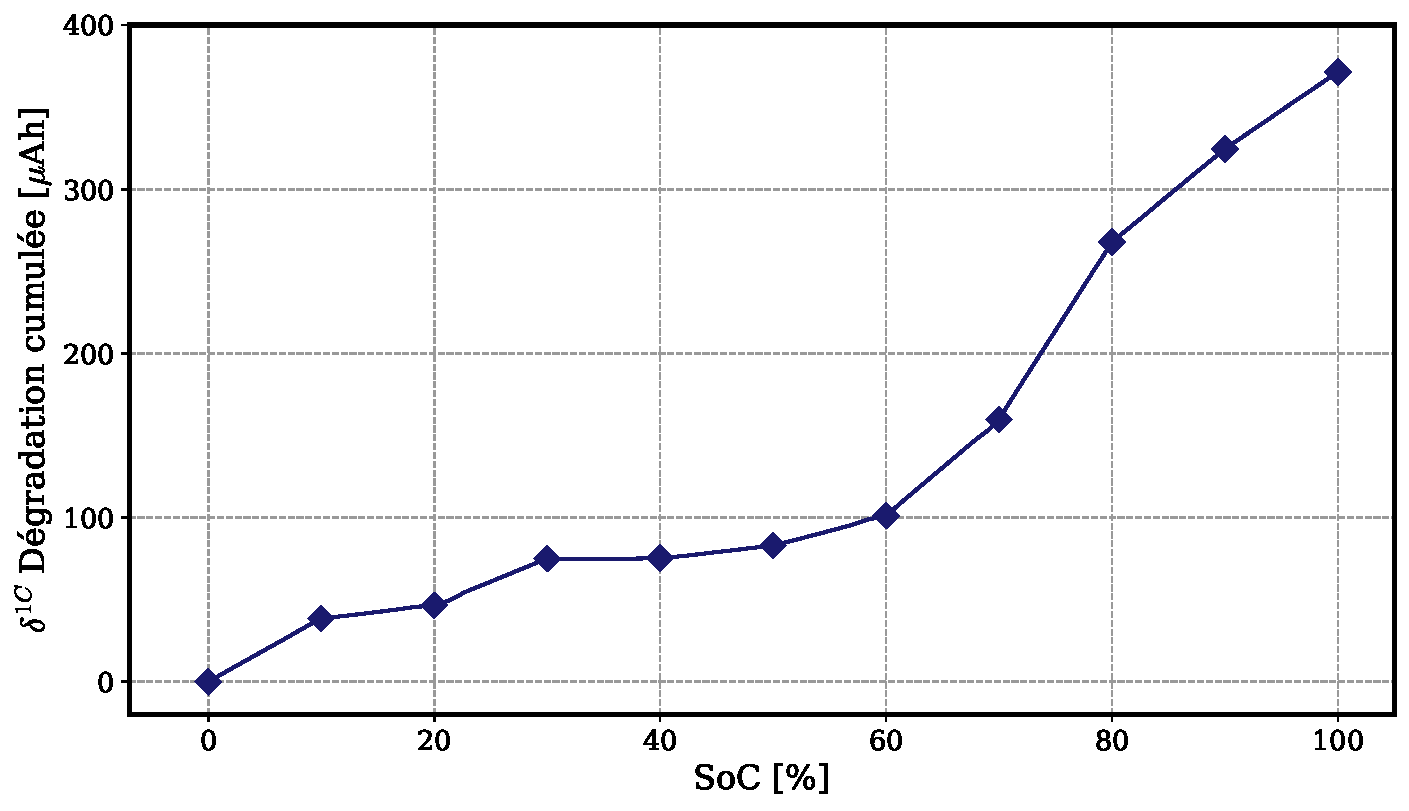
\includegraphics[width=0.8\linewidth]{Chapitre 2/Indicateurs/Figures/batt_deg_dod_cumul.pdf}
    \caption{Dégradation cumulée de la capacité de la batterie induite par le cyclage~\cite{maheshwari_optimizing_2020}.}
    \label{fig:battery_deg}
\end{figure}
\FloatBarrier

La dégradation de référence $d_t^{1\text{C}}$ doit ensuite être corrigée pour intégrer l'effet de l'intensité du courant réel (C-rate), qui accélère le vieillissement en accentuant les contraintes mécaniques (gradients de concentration de lithium, fissuration de l'interface d'électrolyte solide SEI) et les échauffements locaux. Le C-rate effectif $i_t$ auquel est soumis l'accumulateur au pas de temps $t$ est directement calculé à partir du profil de puissance~\cite{maheshwari_optimizing_2020}~:
\begin{equation}
    i_t = \frac{P_t^{ch} + P_t^{dis}}{V_{\text{nom}} \cdot I_{1\text{C}}}
    \label{eq:crate_calculation}
\end{equation}
L'impact de ce courant est modélisé de façon multiplicative par un facteur d'échelle empirique $\psi(i_t)$, indépendant de l'état de charge~\cite{maheshwari_optimizing_2020}. Ce facteur est normalisé pour valoir contractuellement 0 à circuit ouvert (0C, absence de courant de cyclage) et 1 au régime nominal de 1C. À partir des données expérimentales de l'étude d'origine, la progression de ce facteur est interpolée linéairement entre les points de contrôle empiriques pour refléter l'accroissement des dommages à fort régime~\cite{maheshwari_optimizing_2020}~:
\begin{equation}
    \psi(i_t) = 
    \begin{cases} 
      i_t & \text{si } 0 \le i_t \le 1 \\
      1 + 0{,}2956 \cdot (i_t - 1) & \text{si } 1 < i_t \le 2 
    \end{cases}
    \label{eq:psi_crate}
\end{equation}

En combinant l'influence géométrique du cycle (SoC et DoD) et l'intensité du courant, la dégradation effective subie par la batterie à chaque pas de temps, notée $\delta_t$, s'exprime sous la forme du produit fonctionnel suivant~\cite{maheshwari_optimizing_2020}~:
\begin{equation}
    \delta_t = d_t^{1\text{C}} \times \psi(i_t)
    \label{eq:effective_degradation_step}
\end{equation}

Finalement, l'indicateur de dégradation totale accumulée sur l'ensemble du profil de simulation, noté $D_{\text{bat}}$, est obtenu par la sommation directe de ces contributions temporelles~:
\begin{equation}
    D_{\text{bat}} = \sum_t \delta_t
    \label{eq:total_degradation}
\end{equation}

Exprimé de manière absolue en Ampères-heures (Ah) ou en pourcentage de capacité initiale amortie, cet indicateur $D_{\text{bat}}$ synthétise l'impact physique global du profil de puissance appliqué. Il constitue la grandeur d'entrée requise pour la suite des calculs de cette section~: en multipliant cette valeur de capacité perdue par le coût unitaire de remplacement de la batterie (exprimé en €/Ah perdu), il devient possible d'attribuer un coût financier précis, direct et objectif à n'importe quelle séquence opérationnelle imposée au système de stockage.

% - - - - - - - - - - - - - - - - - - - - - - - - - - - - - -
\subsubsection{Piles à combustible}
% - - - - - - - - - - - - - - - - - - - - - - - - - - - - - -

De même que pour les batteries, l'évaluation du coût d'exploitation d'une PEMFC requiert un formalisme capable de traduire un profil opérationnel de puissance en une mesure physique quantifiable du vieillissement. L'indicateur de dégradation globale de la pile à combustible, noté $D_{\text{FC}}$ et développé dans cette sous-section, remplit ce rôle en estimant le taux d'usure cumulé du système, exprimé sous la forme d'un pourcentage de perte de performance ou de chute de tension nominale.

Conformément aux travaux empiriques de Pei \textit{et al.}~\cite{pei_quick_2008} ainsi qu'aux analyses de Foniok \textit{et al.}~\cite{foniok_mechanisms_2025} et de Nguyen \textit{et al.}~\cite{nguyen_comprehensive_2023}, le vieillissement d'une PEMFC en conditions de transport ou de sollicitations stationnaires dynamiques ne dépend pas seulement du temps de fonctionnement linéaire, mais résulte de la superposition de quatre régimes opérationnels principaux et particulièrement contraignants~: les événements de démarrage-arrêt, les périodes de ralenti, les transitoires dynamiques de charge, et le fonctionnement prolongé à forte puissance. L'objectif est ici d'isoler ces contributions afin de quantifier l'état d'usure du système.

L'indicateur de dégradation totale $D_{\text{FC}}$ est ainsi modélisé par une formulation additive découplant l'impact de chacun de ces quatre mécanismes majeurs~\cite{pei_quick_2008}~:
\begin{equation}
    D_{\text{FC}} = d_{\text{start-stop}} + d_{\text{idling}} + d_{\text{transient}} + d_{\text{high power}}
    \label{eq:degradation_fc}
\end{equation}
La superposition additive de mécanismes, chacun affecté d'un taux de chute de tension indépendant, constitue un choix de modélisation répandu pour le vieillissement des PEMFC~\cite{nguyen_comprehensive_2023}\cite{foniok_mechanisms_2025}. Les taux élémentaires de chacune des quatre contributions sont ici calibrés à partir des données expérimentales de Song \textit{et al.}~\cite{song_pontryagins_2020} et exprimés en pourcentage de chute de tension.

Pour formaliser mathématiquement ces contributions sans recourir à des variables binaires d'optimisation, les équations sont définies de manière purement descriptive à partir de la série temporelle de la puissance électrique délivrée par la pile, notée $P_t$, sur un horizon temporel discret discrétisé par pas de temps $\Delta T$. 

La première contribution, $d_{\text{start-stop}}$, comptabilise l'impact des cycles de mise en marche et d'arrêt. Lors de ces phases transitoires, la formation temporaire d'un front hydrogène/air au sein de l'anode engendre localement des potentiels de cathode très élevés (supérieurs à 1,2~V), provoquant une oxydation sévère du support carboné et la dissolution du catalyseur de platine~\cite{foniok_mechanisms_2025}\cite{pei_quick_2008}. En s'appuyant sur les variations d'état opérationnel détectées directement dans le profil, cette dégradation cumulée s'exprime par~\cite{pei_quick_2008}~:
\begin{equation}
    d_{\text{start-stop}} = \sum_t \alpha_{\text{start-stop}} \cdot \max\left(0, \text{sign}(P_t) - \text{sign}(P_{t-1})\right)
    \label{eq:fc_start_stop}
\end{equation}
où $\alpha_{\text{start-stop}}$ désigne le taux de chute de tension élémentaire subi à chaque occurrence de démarrage, calibré sur les données expérimentales de Song \textit{et al.}~\cite{song_pontryagins_2020}.

La deuxième composante, $d_{\text{idling}}$, correspond aux périodes d'attente à vide ou de ralenti. Lorsque la pile fonctionne sous un seuil de puissance minimal, ici fixé à 1\,\% de sa puissance nominale $P_{\text{nom}}$, l'accumulateur opère à une tension de circuit ouvert élevée. Ce haut potentiel thermodynamique favorise la croissance d'oxydes de platine instables et accélère la dégradation chimique de la membrane par la formation de radicaux libres~\cite{nguyen_comprehensive_2023}. Le vieillissement associé est intégré au cours du temps à l'aide d'une fonction indicatrice booléenne $\mathbbm{1}(\cdot)$~\cite{pei_quick_2008}~:
\begin{equation}
    d_{\text{idling}} = \sum_t \alpha_{\text{idling}} \cdot \mathbbm{1}\left(0 < P_t \le 0{,}01 \cdot P_{\text{nom}}\right) \cdot \Delta T
    \label{eq:fc_idling}
\end{equation}
où $\alpha_{\text{idling}}$ représente le taux de dégradation par unité de temps associé à ce régime de basse puissance~\cite{pei_quick_2008}.

La troisième contribution, $d_{\text{transient}}$, quantifie l'effet des variations dynamiques de charge. Les sauts rapides de puissance provoquent des déséquilibres locaux d'approvisionnement en réactifs ainsi que des fluctuations brutales de température et d'humidité relative au sein des cellules. Ces contraintes hydro-mécaniques cycliques induisent des délaminages et des micro-fissures irréversibles au sein de la MEA~\cite{foniok_mechanisms_2025}. L'impact de ces sollicitations transitoires est évalué à partir de la variation absolue de la puissance entre deux pas de temps successifs~\cite{pei_quick_2008}~:
\begin{equation}
    d_{\text{transient}} = \sum_t \alpha_{\text{transient}} \cdot |P_t - P_{t-1}|
    \label{eq:fc_transient}
\end{equation}
où $\alpha_{\text{transient}}$ est un coefficient de proportionnalité empirique traduisant la sévérité des sauts de charge sur la structure interne de la pile.

Enfin, le terme $d_{\text{high power}}$ modélise l'accélération de l'usure induite par une opération continue à des niveaux de charge élevés, définis ici au-delà de 80\,\% de la puissance nominale. À forte densité de courant, la production d'eau interne atteint son maximum, ce qui peut saturer les canaux de diffusion, entraver l'accès des gaz aux sites actifs et induire d'importants gradients thermiques locaux~\cite{nguyen_comprehensive_2023}. Cette dégradation s'accumule de manière proportionnelle à la durée d'exposition~\cite{pei_quick_2008}~:
\begin{equation}
    d_{\text{high power}} = \sum_t \alpha_{\text{high}} \cdot \mathbbm{1}\left(P_t > 0{,}80 \cdot P_{\text{nom}}\right) \cdot \Delta T
    \label{eq:fc_high_power}
\end{equation}
où $\alpha_{\text{high}}$ correspond au taux de dégradation spécifique en régime stationnaire de forte puissance~\cite{pei_quick_2008}.

En effectuant la sommation de ces quatre contributions temporelles autonomes, l'indicateur synthétique $D_{\text{FC}}$ caractérise de manière exhaustive la perte d'intégrité de la pile induite par son profil d'utilisation. Représentant la chute globale de performance, cet indicateur constitue la grandeur d'entrée requise pour la suite des calculs économiques de cette section~: en multipliant ce pourcentage de capacité dégradée par le coût total de remplacement du c\oe ur de la pile à combustible (exprimé en €/\% de perte d'intégrité), il devient possible d'attribuer un coût financier direct et mesurable à n'importe quelle séquence opérationnelle imposée au système.

% - - - - - - - - - - - - - - - - - - - - - - - - - - - - - -
\subsubsection{Électrolyseurs}
% - - - - - - - - - - - - - - - - - - - - - - - - - - - - - -

De manière analogue aux composants précédents, la modélisation du coût d'exploitation d'un PEMWE nécessite de formaliser mathématiquement l'impact d'un profil de puissance sur son intégrité physique. L'indicateur de dégradation globale de l'électrolyseur, noté $D_{\text{ELY}}$, remplit cette fonction en estimant le taux d'usure cumulé du système. Comme pour la pile à combustible, le vieillissement d'un électrolyseur se manifeste par une augmentation progressive de sa tension de cellule à densité de courant constante, traduisant l'accroissement des résistances internes et la perte d'efficacité énergétique du procédé~\cite{endrodi_challenges_2025}\cite{kuhnert_impact_2024}.

Contrairement à une description purement cumulative, le modèle retenu ici, calibré sur les essais de durabilité rapportés par Rakousky \textit{et al.}~\cite{rakousky_polymer_2017}, rend compte du fait qu'une partie de la perte de performance d'un PEMWE est \emph{réversible}. Une contribution \emph{irréversible}, associée à des mécanismes tels que la corrosion de la couche de transport poreuse en titane et la croissance de la résistance ohmique, coexiste avec une contribution \emph{réversible} qui s'accumule en fonctionnement et se résorbe partiellement lorsque le courant est interrompu. Ce modèle intègre par ailleurs les mécanismes de dégradation typiques liés au fonctionnement au ralenti et aux cycles de démarrage-arrêt~\cite{kuhnert_impact_2024}. L'indicateur total s'exprime ainsi comme la somme de quatre termes, tous exprimés en pourcentage d'augmentation de la tension de cellule~:
\begin{equation}
    D_{\text{ELY}} = D_{\text{ELY}}^{\text{irr}} + D_{\text{ELY}}^{\text{rev}} + d_{\text{start-stop}} + d_{\text{idling}}
    \label{eq:degradation_el}
\end{equation}

Chaque composante est calculée de façon déterministe à partir de la série temporelle de la puissance électrique consommée par l'électrolyseur, notée $P_t$, à laquelle correspond une densité de courant $i_t$ sur un horizon discrétisé par pas de temps $\Delta T$. Les deux contributions continues, irréversible et réversible, sont régies par les dynamiques suivantes~\cite{rakousky_polymer_2017}~:
\begin{equation}
    \dot{V}_{\text{irr}} = a(i), \qquad
    \dot{V}_{\text{rev}} = b(i) - k(i)\, V_{\text{rev}}
    \label{eq:ely_irr_rev}
\end{equation}
où $V_{\text{irr}}$ et $V_{\text{rev}}$ désignent respectivement les surtensions irréversible et réversible accumulées, et où $D_{\text{ELY}}^{\text{irr}} = V_{\text{irr}}$ et $D_{\text{ELY}}^{\text{rev}} = V_{\text{rev}}$ en fin de profil. Les taux de génération $a(i)$ et $b(i)$ traduisent l'accélération de l'usure avec l'intensité de la sollicitation~: ils sont \emph{nuls} en deçà de \SI{1}{\ampere\per\centi\meter\squared} (soit environ \SI{30}{\percent} de $P_{\text{max}}$), \emph{croissent linéairement} jusqu'à leur valeur nominale à \SI{2}{\ampere\per\centi\meter\squared} (environ \SI{60}{\percent} de $P_{\text{max}}$), puis \emph{saturent} au-delà. Le taux de récupération $k(i)$, quant à lui, est élevé au voisinage du courant nul, produisant une résorption quasi instantanée de $V_{\text{rev}}$ à l'arrêt, et négligeable en fonctionnement~; il en résulte qu'un usage soutenu à forte puissance dégrade le \textit{stack} pratiquement comme une contrainte à courant constant, sans bénéficier de récupération.

Aux deux termes continus s'ajoutent deux contributions discrètes. Le terme $d_{\text{start-stop}}$ associe une augmentation fixe de tension à chaque transition arrêt~$\rightarrow$~marche (OFF~$\rightarrow$~ON)~: ces transitions provoquent de fortes variations du potentiel de l'anode et favorisent le croisement des gaz à travers la membrane, sources de contraintes chimiques lors de la remise en service~\cite{kuhnert_impact_2024}. Le terme $d_{\text{idling}}$ pénalise le temps passé à très faible puissance, son taux étant tiré des travaux de Lu \textit{et al.}~\cite{lu_optimization_2023}~; dans ce régime, le faible débit de production de gaz accentue leur concentration relative au travers de la membrane et favorise des réactions de recombinaison exothermiques délétères pour le polymère.

En totalisant ces quatre composantes, l'indicateur $D_{\text{ELY}}$ fournit une quantification unifiée de la perte de performance de l'électrolyseur induite par son profil d'utilisation. Exprimé sous la forme d'un pourcentage global d'augmentation de la tension nominale, cet indicateur constitue la variable physique d'entrée pour le calcul économique~: en multipliant cette valeur de dégradation par le coût unitaire de remplacement ou de reconditionnement du \textit{stack}, il devient possible d'affecter un coût financier direct à chaque mode d'exploitation du système. La distinction réversible/irréversible a par ailleurs une conséquence importante pour la gestion d'énergie~: une stratégie qui alterne fréquemment entre forte puissance et arrêt ne paie, pour la part réversible, qu'un coût transitoire largement effacé par la récupération à l'arrêt, tandis qu'un fonctionnement prolongé à forte charge accumule une usure quasi irréversible.

% - - - - - - - - - - - - - - - - - - - - - - - - - - - - - -
\subsubsection{Unification de l'indicateur de dégradations}
% - - - - - - - - - - - - - - - - - - - - - - - - - - - - - -

Une fois les trois indices physiques $D_{\text{bat}}$, $D_{\text{FC}}$ et $D_{\text{ELY}}$ établis, la construction de l'indicateur agrégé $D_{\text{tot}}$ procède en deux temps~: chaque indice est d'abord \emph{normalisé} par le critère de fin de vie du composant correspondant (cf.\ équation~\ref{eq:degradation_total}), de sorte à obtenir une grandeur sans dimension comparable entre technologies~; il est ensuite \emph{pondéré} par le coût financier de remplacement du composant. L'indicateur $D_{\text{tot}}$ représente ainsi une mesure agrégée, homogène à un coût, de la durabilité à long terme d'une stratégie donnée.

Le choix des coefficients de pondération $C_{\text{bat}}$, $C_{\text{FC}}$ et $C_{\text{ELY}}$ mérite une attention particulière, car il conditionne directement le sens économique de l'indicateur agrégé $D_{\text{tot}}$. Dans ce travail, ces coefficients sont calculés à partir de 90\,\% du CAPEX des composants~\cite{noauthor_kpis_nodate}\cite{noauthor_electrolyser_nodate}\cite{noauthor_clean_nodate}~: 90\,\% de la valeur d'achat de la batterie pour $C_{\text{bat}}$, et 90\,\% du coût du stack pour le PEMWE et la PEMFC respectivement. Ce choix reflète la part du coût de remplacement effectivement attribuable à la dégradation en service, en excluant une fraction résiduelle liée à d'autres facteurs (main-d'œuvre, infrastructure, etc.).

Il convient de souligner que ces pondérations sont nécessairement dépendantes du contexte technico-économique et sont susceptibles d'évoluer avec la maturité des technologies. En particulier, le coût des équipements hydrogène (pile à combustible et électrolyseur) est aujourd'hui significativement plus élevé que celui des batteries lithium-ion à capacité énergétique équivalente, ce qui se traduit par un poids plus important des composants hydrogène dans l'indicateur $D_{\text{tot}}$. Cela a pour conséquence d'orienter naturellement les EMS vers une préservation prioritaire de ces équipements, au détriment potentiel d'une sollicitation plus importante de la batterie. Cette sensibilité aux pondérations devra être gardée à l'esprit lors de l'interprétation des résultats présentés dans les sections suivantes~; elle fait l'objet d'une analyse quantitative dédiée à la section~\ref{sec:sensibilite}.

% - - - - - - - - - - - - - - - - - - - - - - - - - - - - - -
\subsubsection{Synthèse}
% - - - - - - - - - - - - - - - - - - - - - - - - - - - - - -

Les trois indices de dégradation partagent une même logique, traduire un profil de puissance en une mesure physique d'usure normalisée puis convertie en coût, mais reposent sur des manifestations physiques distinctes et sont pilotés par des facteurs de stress différents. Le Tableau~\ref{tab:synthese_degradation} en récapitule les éléments saillants. Les facteurs de stress dominants ne sont notamment pas les mêmes selon les composants~: la batterie est surtout sensible au niveau de SoC et à la profondeur des cycles, tandis que les composants hydrogène sont avant tout pénalisés par les transitions de fonctionnement (démarrages-arrêts) et les régimes extrêmes. Cette différence de nature est précisément ce qui ouvre la voie à des arbitrages de gestion d'énergie~: répartir judicieusement la sollicitation entre batterie et hydrogène permet de ménager simultanément des mécanismes d'usure qui ne répondent pas aux mêmes causes.

\begin{table}[h!]
\centering
\caption{Synthèse des indicateurs de dégradation~: manifestation du vieillissement, critère de fin de vie et principaux facteurs de dégradation.}
\label{tab:synthese_degradation}
\footnotesize
\renewcommand{\arraystretch}{1.25}
\begin{tabularx}{\textwidth}{p{2.1cm} p{3.5cm} X}
\hline
\textbf{Composant} & \textbf{Manifestation / critère EoL} & \textbf{Principaux facteurs de dégradation} \\ \hline
Batterie & Perte de capacité~; EoL à \SI{-30}{\percent} (SoH \SI{70}{\percent}) & Niveau de SoC, profondeur de décharge (DoD), régime de courant (C-rate). \\
PEMFC & Chute de tension à courant constant~; EoL à \SI{+10}{\percent} & Cycles de démarrage-arrêt (dominants), ralenti, transitoires de puissance, fonctionnement à forte puissance. \\
PEMWE & Hausse de tension à courant constant~; EoL à \SI{+10}{\percent} & Composantes réversible/irréversible, cycles de démarrage-arrêt, ralenti, fonctionnement soutenu à forte puissance. \\ \hline
\end{tabularx}
\end{table}
\FloatBarrier

% ============================================================
%  CHAPITRE 2 — Section : Approche réactive au vieillissement
% ============================================================

\section{Approche réactive au vieillissement}
\label{sec:soh}

Le chapitre précédent a établi, pour chacun des trois composants de stockage, une définition scalaire de l'état de santé ainsi que les méthodes permettant de l'estimer en ligne. Cet état de santé correspond à la capacité résiduelle relative pour la batterie et à la perte (resp.\ augmentation) relative de puissance à courant constant pour la pile à combustible (resp.\ l'électrolyseur)~; il est estimé par le suivi de la résistance interne pour la batterie et par des observateurs de type filtre de Kalman étendu pour les composants hydrogène. Ces estimations sont supposées disponibles, dans la suite, à une cadence au moins hebdomadaire, ce qui est largement suffisant au regard des constantes de temps du vieillissement (plusieurs mois à plusieurs années).

Il importe de bien distinguer ces indicateurs de SoH des indices de dégradation de la section~\ref{sec:indicateurs}. Les seconds servent à \emph{évaluer a posteriori} la durabilité d'une EMS~; les premiers servent à \emph{informer le contrôle} en temps réel. C'est ce second usage qui est considéré ici. En effet, le vieillissement réduit les capacités physiques des composants~: la capacité utile de la batterie diminue, et la puissance maximale délivrable par les composants hydrogène à courant donné se dégrade. Les plages de fonctionnement nominales, définies à la mise en service, deviennent donc progressivement inadaptées~; continuer à émettre des consignes calibrées sur l'état neuf reviendrait à demander des puissances physiquement irréalisables.

L'\emph{approche réactive} adoptée dans ce chapitre consiste à exploiter le SoH estimé pour \emph{actualiser en continu les bornes physiques} (puissances maximales, capacité, bande de SoC) utilisées par le contrôle de faisabilité de l'EMS. Cette actualisation est défensive et \emph{commune à toutes les stratégies} examinées~: quelle que soit la logique de répartition, le contrôle doit rester dans l'enveloppe de fonctionnement réelle, évolutive, des composants. L'information de vieillissement n'est donc utilisée ici que pour garantir la faisabilité des commandes, sans modifier la logique de répartition. Elle se distingue en cela de l'approche \emph{anticipative} du chapitre suivant, où le SoH et la RUL sont injectés dans les règles de décision pour moduler proactivement la sollicitation des composants. L'approche réactive constitue le socle commun sur lequel cette extension anticipative viendra ensuite s'appuyer.

% ============================================================
%  CHAPITRE 2 — Section 3 : Cadre d'évaluation & comparaison des EMS
% ============================================================

\section{Cadre d'évaluation \& comparaison des EMS}
\label{sec:simulation}

Les indicateurs définis dans les sections précédentes permettent de caractériser quantitativement la performance de toute EMS selon deux axes principaux~: la fiabilité d'alimentation à court terme (LPSP) et le coût de dégradation à long terme ($D_{\text{tot}}$). Il reste à définir le cadre dans lequel ces indicateurs sont calculés et exploités pour comparer les stratégies entre elles. Cette section décrit successivement la représentation graphique adoptée pour la comparaison des EMS (le plan de Pareto) et l'algorithme de simulation qui en permet le calcul. La troisième dimension de robustesse aux défaillances, sera traitée à la section~\ref{sec:robustesse}.

% ------------------------------------------------------------
\subsection{Représentation dans l'espace de performance (plan de Pareto)}
% ------------------------------------------------------------

À l'issue de chaque simulation, une EMS est entièrement caractérisée par le couple $(\mathrm{LPSP},\, D_{\text{tot}})$ qu'elle produit sur l'horizon de simulation. Il est alors naturel de représenter l'ensemble des EMS étudiées comme des points dans un espace de performance bidimensionnel, dont les axes correspondent respectivement à la LPSP (axe horizontal) et au coût de dégradation agrégé $D_{\text{tot}}$ exprimé en euros (axe vertical). Cette représentation constitue un plan de Pareto au sens large~: le point idéal, correspondant à une LPSP nulle et un coût de dégradation nul, se situe à l'origine, et toute amélioration sur un axe se fait en général au détriment de l'autre.

Cette visualisation présente plusieurs avantages pour la comparaison des EMS. D'une part, elle permet d'identifier immédiatement les stratégies dominées, c'est-à-dire celles pour lesquelles il existe une autre EMS offrant de meilleures performances sur les deux axes simultanément. D'autre part, elle met en évidence le front de Pareto, c'est-à-dire l'ensemble des EMS non dominées qui définissent la frontière des compromis réalisables~: toute amélioration d'un indicateur implique nécessairement une dégradation de l'autre. Enfin, cette représentation est particulièrement adaptée à la communication des résultats auprès des opérateurs ou des populations locales, à qui il appartient in fine de choisir le niveau de compromis acceptable entre confort d'alimentation et coût de maintenance.

Il est important de noter que certaines EMS peuvent ne pas être strictement dominées au sens de Pareto tout en étant peu attractives en pratique, par exemple si elles se trouvent très éloignées du front de compromis. L'interprétation de ce plan doit donc toujours s'accompagner d'une analyse du contexte applicatif et des priorités locales.

% ------------------------------------------------------------
\subsection{Algorithme de simulation}
% ------------------------------------------------------------

Le calcul des indicateurs de performance repose sur un algorithme de simulation en boucle fermée, dont le déroulement à l'intérieur d'un pas de temps est illustré à la Figure~\ref{fig:workflow}. À chaque pas de temps $t$, l'EMS établit une application de l'état instantané du système vers les consignes de contrôle. L'état instantané comprend le SoC de la batterie, le niveau d'hydrogène stocké $E_{\text{H2}}$, l'état de santé estimé des composants de stockage, ainsi que la demande de charge planifiée $\hat{P}_{\text{Load}}$ et la production PV $\hat{P}_{\text{PV}}$ à cet instant~; les consignes de contrôle sont les puissances des composants de stockage $\tilde{P}_{\text{bat}}(t)$, $\tilde{P}_{\text{FC}}(t)$ et $\tilde{P}_{\text{ELY}}(t)$.

Concrètement, l'EMS calcule d'abord la demande nette planifiée $\hat{P}_{\text{tot,plan}} = \hat{P}_{\text{Load}} - \hat{P}_{\text{PV}}$ puis, selon son signe (déficit ou surplus), applique un bloc de règles propre à la stratégie qui affecte la consigne du côté hydrogène, la batterie assurant le complément. Ce bloc de règles est générique~: n'importe laquelle des stratégies décrites à la section~\ref{sec:ems} peut y être insérée. Les consignes ainsi obtenues passent ensuite par un contrôle de faisabilité au regard des limites de fonctionnement~: puissances maximales des composants (actualisées par le SoH, cf.\ section~\ref{sec:soh}), bande de SoC admissible et capacité du réservoir d'hydrogène. Lorsque la commande demandée est infaisable, elle est saturée à ces limites. C'est précisément cette saturation qui peut créer une discordance entre la puissance planifiée et la puissance effectivement délivrée, et donc une perte d'alimentation contribuant à la LPSP. Une fois la commande faisable obtenue, les équations dynamiques régissant le comportement des composants sont résolues sur le pas de temps courant afin d'obtenir l'état du système au pas de temps suivant.

\begin{figure}[h!]
    \centering
    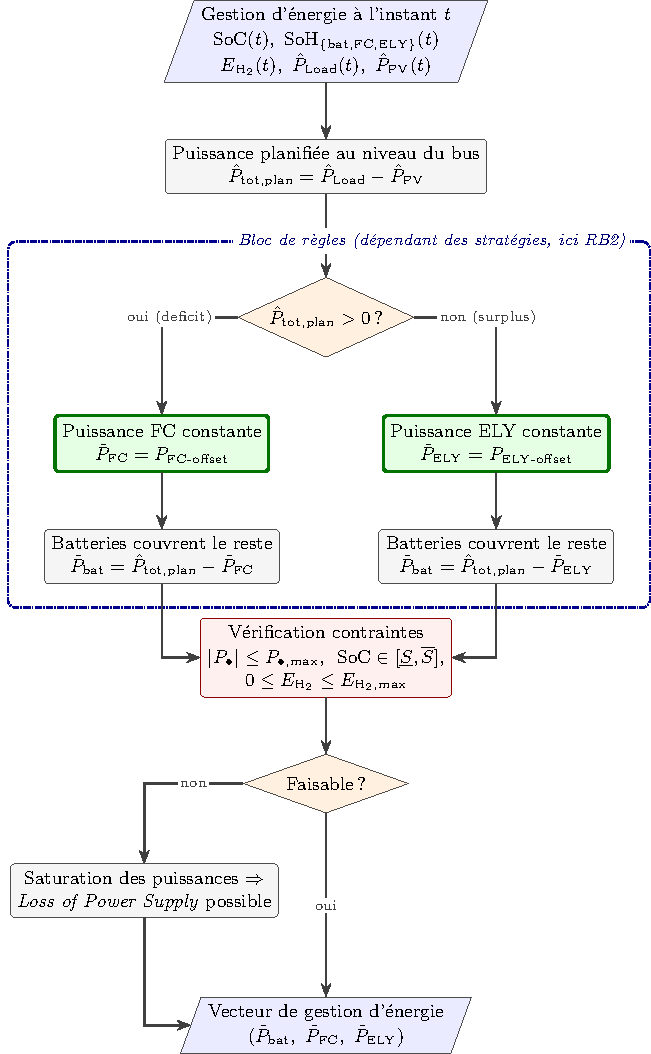
\includegraphics[width=.5\linewidth]{Chapitre 2/Simulation/Figures/workflow_ems_fr.pdf}
    \caption{Déroulé de la stratégie de gestion d'énergie sur un pas de temps $t$.}
    \label{fig:workflow}
\end{figure}
\FloatBarrier

Ce processus est répété sur l'intégralité de l'horizon de simulation, dont la durée est fixée à vingt-cinq ans. Ce choix permet d'observer clairement les processus de vieillissement à l'œuvre dans les composants de stockage, en incluant plusieurs remplacements de composants, tout en maintenant un temps de calcul raisonnable. Les simulations ont été implémentées en Python 3.12 et exécutées sur un poste de travail Intel Xeon W-2123 (4 cœurs, 3,60\,GHz, 32\,Go de RAM), avec un temps de calcul moyen d'environ dix minutes par simulation.

Le pas de temps de simulation est fixé à une heure. Seul le contrôle échantillonné à cette résolution est considéré dans ce travail~; le contrôle aux échelles de temps inférieures est supposé assuré par une couche de contrôle distincte. Les demandes de puissance à l'intérieur d'un intervalle d'une heure sont donc considérées comme constantes. Il convient toutefois de reconnaître que cette résolution temporelle peut conduire à une sous-estimation partielle des fluctuations de puissance infra-horaires, et par conséquent de certains phénomènes de dégradation survenant dans des conditions de fonctionnement plus rapides~\cite{e_toosi_impact_2023}\cite{pei_quick_2008}.

L'ensemble des simulations est réalisé dans les mêmes conditions environnementales et avec les mêmes modèles de composants, afin de garantir la comparabilité des résultats. Les profils de puissance PV et de demande de charge sont issus de données représentatives du microréseau résidentiel de La Réunion présenté au chapitre précédent. Il est par ailleurs supposé que l'estimation du SoH des composants est suffisamment précise pour que les plages de fonctionnement associées correspondent à la réalité.

À l'issue de la simulation, chaque EMS est représentée par un unique point dans le plan de Pareto décrit à la sous-section précédente. Ce cadre est appliqué à chaque stratégie considérée, permettant une comparaison directe et visuelle de l'ensemble des EMS étudiées. Ce cadre intègre par ailleurs, pour chaque stratégie, l'approche réactive au vieillissement décrite à la section~\ref{sec:soh}~: les plages de fonctionnement utilisées par le contrôle de faisabilité sont actualisées à chaque pas en fonction du SoH estimé des composants.

% ============================================================
%  CHAPITRE 2 — Section 4 : EMS considérées
% ============================================================

\section{EMS considérées}
\label{sec:ems}

Cette section présente les différentes EMS qui ont été conçues et simulées dans le cadre d'évaluation décrit précédemment. L'objectif est d'explorer un éventail de philosophies de contrôle suffisamment large pour couvrir les principaux compromis réalisables dans le plan de Pareto, et d'identifier parmi elles la stratégie offrant le meilleur équilibre entre fiabilité d'alimentation et préservation des composants. Toutes les EMS présentées ici sont des stratégies en ligne, c'est-à-dire qu'elles ne s'appuient pas sur la connaissance du futur et sont compatibles avec une implémentation temps réel dans le microréseau.

% ------------------------------------------------------------
\subsection{Power-splitting \& frequency splitting}
% ------------------------------------------------------------

La première famille de stratégies repose sur une répartition statique de la puissance entre la batterie et le sous-système hydrogène. Ces configurations sont caractérisées par des ratios de distribution fixes de la puissance de référence totale $\hat{P}_{\text{tot,plan}} = (\hat{P}_{\text{Load}} - \hat{P}_{\text{PV}})$ entre les deux médias de stockage~:
\[
(100-0), \quad (75-25), \quad (50-50), \quad (25-75), \quad (0-100)
\]
où le premier terme correspond à la part [\%] attribuée à la batterie et le second au système hydrogène. Ces stratégies vont donc d'une philosophie attribuant l'essentiel du travail à la batterie à une philosophie le confiant principalement aux composants hydrogène~\cite{eldeeb_hybrid_2019}.

Cette approche est structurellement proche des stratégies de \textit{frequency splitting}, dans lesquelles deux composants de stockage aux dynamiques temporelles différentes se partagent différentes bandes du spectre fréquentiel de la charge~\cite{corapsiz_overview_2023}. Dans ce type de stratégie, la batterie, plus rapide, absorbe les fluctuations hautes fréquences, tandis que le système hydrogène, plus lent, gère les composantes basses fréquences. Le \textit{power splitting} a toutefois été préféré ici au \textit{frequency splitting}, car il conduit à de meilleurs résultats sur les indicateurs retenus pour ce cas d'étude particulier.

% ------------------------------------------------------------
\subsection{SoC-based}
% ------------------------------------------------------------

Deux lois de contrôle supplémentaires ont été implémentées pour maintenir le SoC de la batterie autour de cibles spécifiques. La première vise à maintenir $\text{SoC}_{\text{bat}}$ proche de $0{,}6$ (notée SoC06), ce qui représente un état équilibré permettant à la fois des marges de charge et de décharge. La seconde cherche à maintenir $\text{SoC}_{\text{bat}}$ proche de $1$ (SoC1), favorisant la disponibilité de l'énergie stockée pour les consommateurs, mais pouvant accroître la dégradation en raison d'un fonctionnement prolongé à SoC élevé. Ces philosophies de contrôle sont également des approches très répandues dans les systèmes électriques hybrides~\cite{sorrentino_real-time_2021}\cite{zou_real-time_2023}.

Dans ces deux stratégies, le sous-système hydrogène joue un rôle d'appui à la batterie~: la pile à combustible est sollicitée pour recharger la batterie lorsque son SoC descend en dessous de la cible, et l'électrolyseur absorbe l'excès de production PV lorsque la batterie est pleine. Cette dépendance forte vis-à-vis des composants hydrogène a des conséquences directes sur leur niveau de sollicitation et donc sur leur dégradation, comme le montreront les résultats.

% ------------------------------------------------------------
\subsection{Autres stratégies}
% ------------------------------------------------------------

Des stratégies à base de règles plus élaborées ont également été implémentées afin de concilier réactivité dynamique et simplicité de calcul. Ces deux stratégies, notées RB1 et RB2, sont décrites ci-après et illustrées à la Figure~\ref{fig:RB_ems}.

\paragraph{Stratégie RB1.}
La stratégie RB1 définit le partage de puissance en fonction du SoC de la batterie au travers de règles par morceaux. Lorsque le SoC se trouve dans la plage intermédiaire ($0{,}2 < \text{SoC}_{\text{bat}} < 0{,}6$), la puissance de référence totale $\hat{P}_{\text{tot,plan}}$ est répartie linéairement entre la batterie et les composants hydrogène~: la batterie fournit la totalité de la puissance de référence lorsque le SoC atteint $0{,}6$, et aucune puissance lorsqu'il atteint $0{,}2$. En dehors de cette plage, la batterie fonctionne seule lorsque $\text{SoC}_{\text{bat}} > 0{,}6$ en décharge ou lorsque $\text{SoC}_{\text{bat}} < 0{,}2$ en charge, tandis que la pile à combustible ou l'électrolyseur prend le relais selon le sens du bilan de puissance. Cette règle assure ainsi des transitions douces entre les différents modes de fonctionnement tout en évitant les valeurs extrêmes de SoC.

\paragraph{Stratégie RB2.}
La stratégie RB2 simplifie la logique de contrôle en définissant deux modes de fonctionnement principaux. Lorsque la puissance de référence totale $\hat{P}_{\text{tot,plan}}$ est positive (la demande de charge excède la production), une puissance d'offset fixe $P_{\text{FC-offset}}$ est allouée à la pile à combustible, et la batterie fournit le complément. De façon symétrique, lorsque $\hat{P}_{\text{tot,plan}}$ est négative (excès de production), l'électrolyseur absorbe une puissance d'offset fixe $P_{\text{ELY-offset}}$, tandis que la batterie assure le reste. Ces paramètres d'offset sont ajustés par recherche des meilleures valeurs d'indicateurs. Cette logique permet aux composants hydrogène de fonctionner à des puissances plus constantes, limitant ainsi les transitoires et les cycles de démarrage-arrêt, et par conséquent prolongeant leur durée de vie.

\begin{figure}[h!]
    \centering
    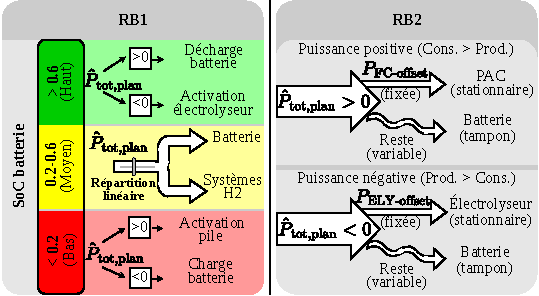
\includegraphics[width=0.8\linewidth]{Chapitre 2/EMS/Figures/RB1_2_EMS_v4.pdf}
    \caption{Illustration des stratégies RB1 et RB2.}
    \label{fig:RB_ems}
\end{figure}
\FloatBarrier

L'ensemble des neuf EMS considérées est récapitulé dans le Tableau~\ref{tab:EMS}.

\begin{table}[h!]
    \centering
    \caption{Récapitulatif des EMS implémentées.}
    \label{tab:EMS}
    \setlength{\tabcolsep}{3pt}
    \begin{tabularx}{\columnwidth}{llX}
        \hline
        Type d'EMS & Notation & Remarques \\
        \hline
        Power split & (X-Y) & $X, Y \in \{0, 25, 50, 75, 100\}$ [\%], parts batterie-hydrogène. \\
        \noalign{\smallskip}
        SoC cible & SoCX & $X \in \{0{,}6\,;\,1\}$~: SoC cible pour la batterie. \\
        \noalign{\smallskip}
        Règles élaborées & RBX & $X \in \{1, 2\}$~: logique décrite à la Fig.~\ref{fig:RB_ems}. \\
        \hline
    \end{tabularx}
\end{table}

% ------------------------------------------------------------
\subsection{Paramètres de simulation \& hypothèses}
% ------------------------------------------------------------

Les paramètres principaux de simulation ainsi que les hypothèses retenues sont rappelés ici pour mémoire, l'algorithme de simulation ayant été décrit à la section précédente. Le système modélisé est le microréseau hybride DC isolé de La Réunion, dont l'architecture et le dimensionnement ont été présentés au chapitre précédent. Les principales données de dimensionnement sont rappelées dans le Tableau~\ref{tab:system_parameters} pour faciliter la lecture des résultats.

\begin{table}[h!]
    \centering
    \caption{Principaux paramètres et dimensionnement du microréseau hybride.}
    \label{tab:system_parameters}
    \begin{tabular}{lcr}
        \hline
        Description & Symbole & Valeur nominale \\
        \hline
        Puissance de charge moyenne         & $\overline{P}_{\text{Load}}$  & 2,2 kW  \\
        Puissance de charge maximale        & $P_{\text{Load,max}}$         & 4,2 kW  \\
        Puissance PV maximale               & $P_{\text{PV,max}}$           & 32,7 kW \\
        Capacité nominale de la batterie    & $E_{\text{bat,nom}}$          & 39 kWh  \\
        Puissance nominale PEMFC            & $P_{\text{FC,max}}$           & 1,5 kW  \\
        Puissance nominale PEMWE            & $P_{\text{ELY,max}}$          & 16 kW   \\
        Capacité de stockage hydrogène      & $E_{\text{H2,max}}$           & 200 kWh \\
        \hline
    \end{tabular}
\end{table}

L'analyse est conduite à dimensionnement fixé~: les tailles des composants ne varient pas d'une simulation à l'autre, ce qui garantit que les différences observées entre EMS sont uniquement imputables aux décisions de contrôle et non à des effets de dimensionnement. Ce choix, bien qu'il ne reflète pas nécessairement une configuration physiquement ou économiquement optimisée, permet une comparaison claire et équitable des stratégies. Les profils de puissance utilisés sont issus de relevés de terrain réalisés à La Réunion, reflétant les habitudes de consommation des résidents locaux et la production solaire caractéristique du site.

Concernant les méthodes d'estimation du SoH, détaillées à la section~\ref{sec:soh}, il est supposé que les techniques existantes permettent un suivi suffisamment précis pour que les plages de fonctionnement actualisées correspondent à la réalité. Cette hypothèse, qui fonde l'approche réactive au vieillissement commune à toutes les EMS, est éprouvée à la section~\ref{sec:sensibilite} au regard d'un bruit sur l'estimation du SoH.

% ------------------------------------------------------------
\section{Résultats préliminaires}
% ------------------------------------------------------------
\subsection{LPSP et dégradation des composants }
\label{sec:resultats}
L'ensemble des neuf EMS décrites ci-dessus a été simulé sur un horizon de vingt-cinq ans, et leurs performances sont représentées dans le plan de Pareto à la Figure~\ref{fig:pareto}. Cette sous-section en présente d'abord les résultats nominaux, lorsque tous les composants sont opérationnels, avant d'en discuter les enseignements et les implications économiques.

% ------------------------------------------------------------
\subsubsection{Résultats}
\label{subsec:pareto_resultats}
% ------------------------------------------------------------

\begin{figure}[h!]
    \centering
    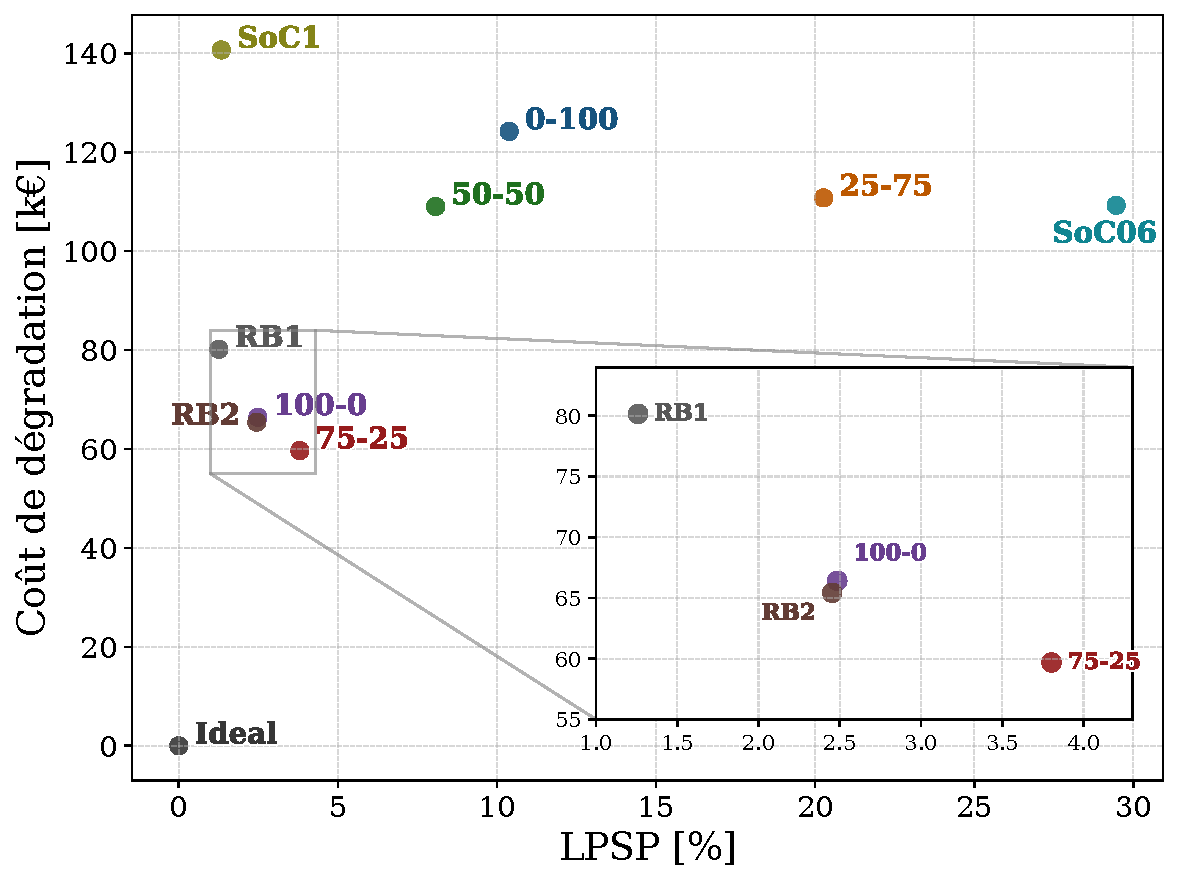
\includegraphics[width=.8\linewidth]{Chapitre 2/EMS/Figures/pareto_ems.pdf}
    \caption{Visualisation des neuf EMS dans le plan de Pareto pour une simulation de vingt-cinq ans.}
    \label{fig:pareto}
\end{figure}
\FloatBarrier

Plusieurs enseignements se dégagent de cette représentation. Les stratégies de \textit{power splitting} apparaissent déjà pertinentes, mais leurs performances sont, comme attendu, fortement dépendantes de la part de puissance assurée par la batterie. Il a été observé qu'une utilisation plus importante de la batterie conduit à une réduction significative des coûts de dégradation~: environ $-46{,}5\,\%$ en passant de l'EMS $0$-$100$ (124~k€) à l'EMS $100$-$0$ (66~k€), les composants hydrogène étant particulièrement sujets à la dégradation. Cette tendance s'accompagne également d'une nette amélioration de la qualité de service ($-76{,}1\,\%$ de LPSP, qui chute de $10{,}4\,\%$ à $2{,}5\,\%$). Ce résultat s'explique par le fait que la batterie, grâce à ses meilleures propriétés dynamiques, est plus à même de répondre rapidement aux fluctuations de charge, là où les composants hydrogène peinent à suivre des variations rapides sans s'user prématurément.

Les stratégies à SoC cible offrent des résultats plus extrêmes. Selon la valeur cible retenue, elles peuvent se révéler à la fois les meilleures et les moins bonnes stratégies en termes de LPSP, mais s'accompagnent systématiquement de coûts de dégradation élevés. La stratégie SoC1, qui maintient la batterie quasiment pleine, atteint une excellente disponibilité (LPSP $\approx 1{,}3\,\%$) mais au prix du coût de dégradation le plus élevé du panel ($\approx 141$~k€)~: garder la batterie à plein SoC impose en effet de solliciter en permanence la pile à combustible pour la recharger, et expose en outre la batterie à un vieillissement calendaire accru. À l'opposé, SoC06, qui vise un SoC médian, dégrade fortement le service (LPSP $\approx 29\,\%$) car elle écrête volontiers l'énergie disponible pour rester proche de la cible, privant les usagers d'une réserve pourtant présente. Ce comportement s'explique, dans les deux cas, par le fait que les composants hydrogène sont entièrement asservis au maintien de la cible de SoC, ce qui les soumet à une sollicitation intense et régulière, délétère pour leur durée de vie.

La stratégie RB1, qui module continûment le partage en fonction du SoC, réalise quant à elle la plus faible LPSP de toutes les stratégies ($\approx 1{,}3\,\%$) pour un coût de dégradation intermédiaire ($\approx 80$~k€). Elle illustre l'intérêt d'une transition douce entre modes de fonctionnement~; son coût reste toutefois supérieur à celui de RB2, car ses transitions progressives sollicitent davantage les composants hydrogène en régime variable que l'offset constant de RB2.

Parmi toutes les stratégies testées, la stratégie à base de règles RB2 apparaît comme offrant le compromis le plus équilibré entre continuité de service et longévité des composants. Elle atteint une LPSP d'environ $2{,}45\,\%$ pour un coût de dégradation d'environ $65{,}4$~k€, se positionnant ainsi près du front de Pareto tout en maintenant des niveaux de LPSP et de dégradation raisonnables. Elle domine notamment légèrement l'EMS $100$-$0$, dont elle reprend la philosophie « tout-batterie » mais qu'elle améliore en allouant aux composants hydrogène une puissance d'offset constante, plus douce pour leur vieillissement. Ce caractère équilibré fait de RB2 la candidate la plus prometteuse en vue d'une amélioration ultérieure.

Le fonctionnement de la stratégie RB2 sur l'horizon complet est illustré à la Figure~\ref{fig:rb2_curves}, qui présente l'évolution des puissances sur vingt-cinq ans ainsi qu'un agrandissement sur une semaine. La batterie y absorbe l'essentiel des fluctuations rapides du déséquilibre entre production et demande, tandis que la pile à combustible et l'électrolyseur fonctionnent par paliers, à une puissance d'offset sensiblement constante entrecoupée de phases d'arrêt. Le suivi du SoC de la batterie et du niveau du réservoir d'hydrogène confirme que les réserves restent dans des plages de fonctionnement saines, les pertes d'alimentation demeurant rares et de faible amplitude.

\begin{figure}[h!]
    \centering
    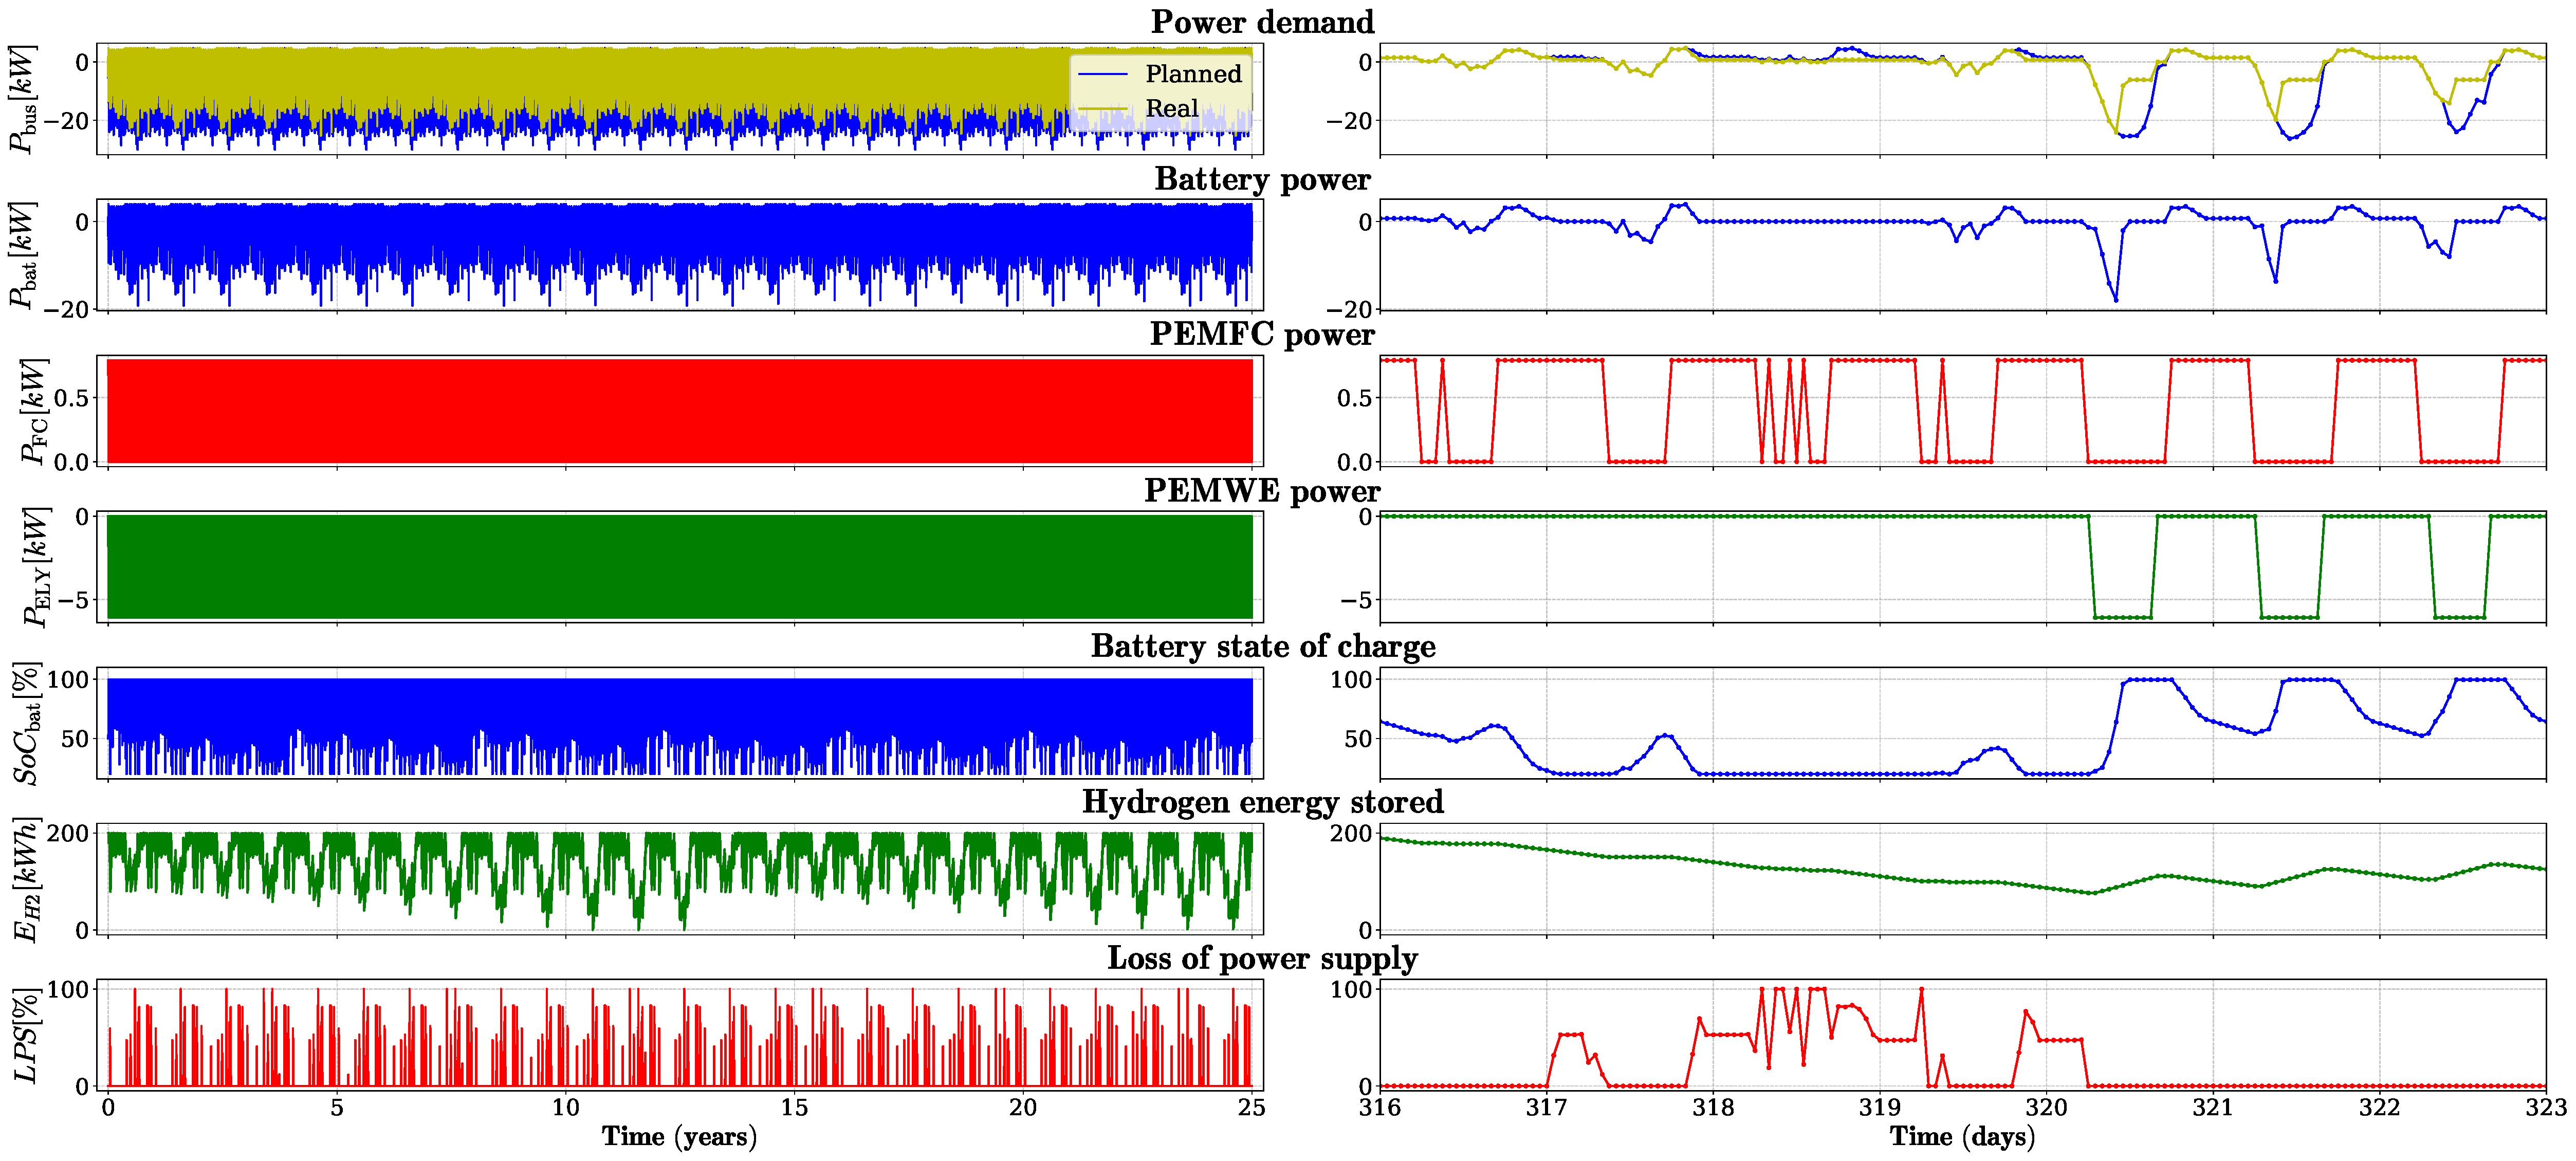
\includegraphics[width=\linewidth]{Chapitre 2/EMS/Figures/everything_combined_v2_2.pdf}
    \caption{Profils de puissance de la stratégie RB2~: simulation sur vingt-cinq ans (gauche) et agrandissement sur une semaine (droite).}
    \label{fig:rb2_curves}
\end{figure}
\FloatBarrier

L'évolution du vieillissement des composants et la décomposition de leur dégradation sont reportées à la Figure~\ref{fig:rb2_aging}. Les courbes de SoH font apparaître les remplacements périodiques évoqués plus haut, la batterie étant de loin le composant le plus fréquemment remplacé. La répartition des mécanismes de dégradation est plus instructive encore~: pour la pile à combustible, les cycles de démarrage-arrêt constituent de loin la cause dominante, avec près de $96\,\%$ de la dégradation totale~; pour l'électrolyseur, la dégradation est principalement portée par la contribution irréversible associée au fonctionnement soutenu à forte puissance (environ $59\,\%$), les démarrages-arrêts n'en représentant qu'environ $36\,\%$.

\begin{figure}[h!]
    \centering
    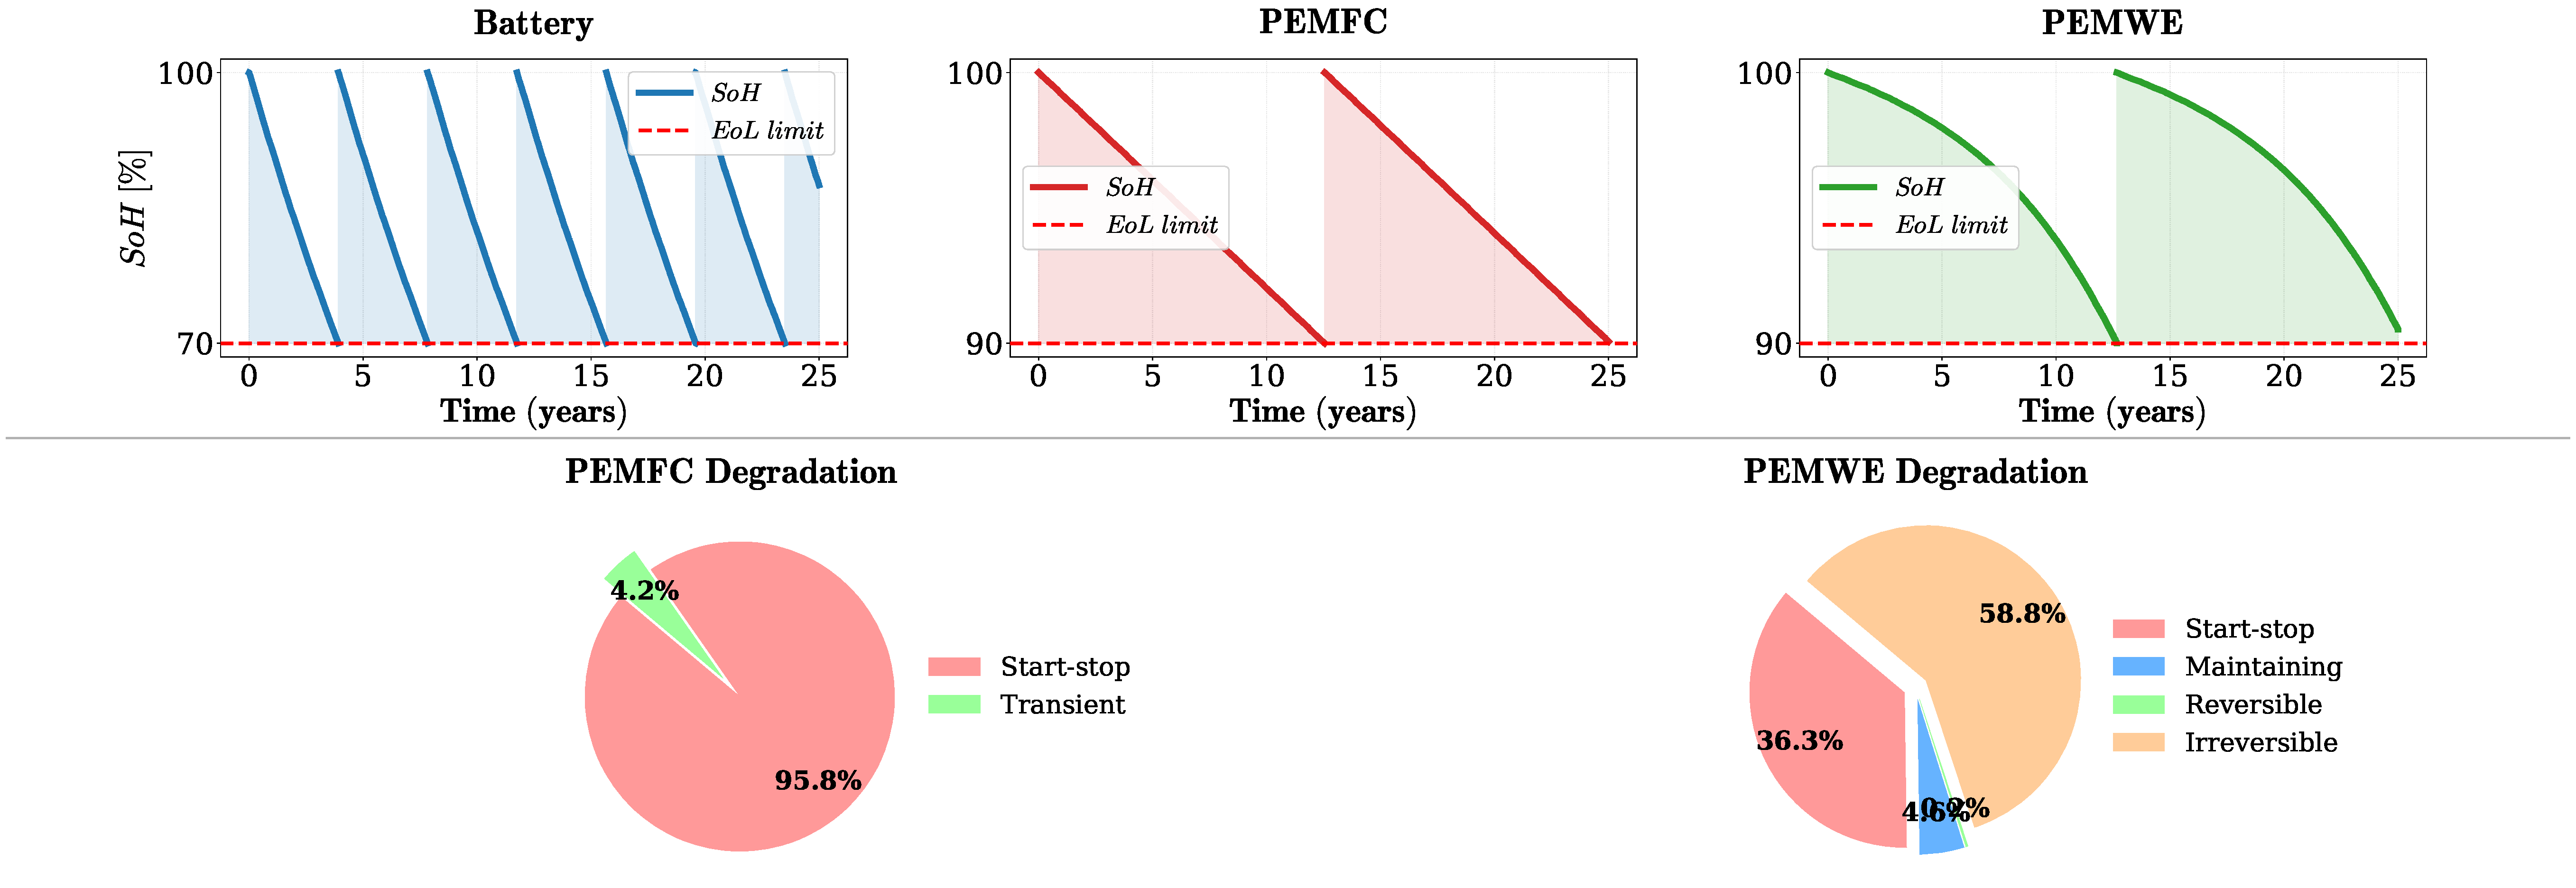
\includegraphics[width=\linewidth]{Chapitre 2/EMS/Figures/all_aging_2.pdf}
    \caption{Vieillissement sous la stratégie RB2~: évolution du SoH des composants (haut) et répartition des mécanismes de dégradation des composants hydrogène (bas).}
    \label{fig:rb2_aging}
\end{figure}
\FloatBarrier

% ------------------------------------------------------------
\subsubsection{Discussion}
% ------------------------------------------------------------

D'un point de vue économique, les coûts équivalents associés à la dégradation des composants s'échelonnent, sur vingt-cinq ans, de l'ordre de 60~k€ à près de 141~k€ selon l'EMS retenue, ce qui souligne l'importance cruciale du choix de la stratégie de contrôle pour l'opération du système. Ces coûts sont liés aux remplacements périodiques des composants, dont les fréquences sont estimées à environ une fois tous les quatre ans pour la batterie, tous les douze à treize ans pour la pile à combustible et tous les treize ans pour l'électrolyseur. Le vieillissement relativement rapide de la batterie est cohérent avec la chimie lithium-ion NMC considérée et avec son dimensionnement modeste, qui impose des cycles profonds et fréquents~; ces durées de vie absolues doivent toutefois être lues comme des estimations dépendantes du modèle et du dimensionnement plutôt que comme des valeurs validées expérimentalement~\cite{madani_comprehensive_2025}\cite{superchi_importance_2025}. La LPSP associée varie quant à elle de l'ordre de $1\,\%$ (RB1) à environ $29\,\%$ (SoC06) selon les stratégies les plus extrêmes, ce qui représente concrètement une indisponibilité de l'alimentation électrique entre $1\,\%$ et $29\,\%$ du temps pour les consommateurs.

La décomposition des mécanismes de dégradation (Figure~\ref{fig:rb2_aging}) éclaire enfin les leviers d'amélioration disponibles. Des essais complémentaires ont été menés pour déterminer si maintenir les composants hydrogène au ralenti lors des faibles sollicitations, plutôt que de les arrêter complètement, permettrait de limiter leur usure~; pour la pile à combustible comme pour l'électrolyseur, le résultat est inverse~: rester au ralenti dégrade davantage les composants qu'un cycle de démarrage-arrêt, ce qui conforte le recours à des phases d'arrêt franches. La prééminence du fonctionnement à forte puissance pour l'électrolyseur, relevée plus haut, suggère quant à elle qu'une réduction de sa puissance de sollicitation constituerait un levier direct de durabilité, piste exploitée au chapitre suivant.

Il est à noter que les EMS ne sont pas strictement dominées au sens de Pareto, et que le choix de la stratégie la plus adaptée n'est donc pas trivial. Il reviendra aux populations locales ou à l'opérateur du système de décider si la priorité doit être accordée au coût financier associé à la dégradation à long terme ou à la commodité à court terme liée à une alimentation plus fiable.

Au terme de cette comparaison, la stratégie RB2 s'impose comme la meilleure stratégie statique du panel~: c'est elle qui semble réaliser le meilleur compromis global entre fiabilité et durabilité. Avant de chercher à l'améliorer, il convient toutefois de soumettre l'ensemble des stratégies à deux examens complémentaires que le plan de Pareto nominal ne permet pas de trancher~: leur comportement face à une défaillance de composant (section~\ref{sec:robustesse}) et la robustesse de leur classement aux hypothèses de modélisation (section~\ref{sec:sensibilite}). Ce n'est qu'une fois cette stratégie de référence consolidée que ses performances seront augmentées, au chapitre suivant, en intégrant directement dans ses règles l'information de diagnostic et de pronostic d'état de santé développée au chapitre précédent.

% ============================================================
%  CHAPITRE 2 — Section : Analyse de robustesse face aux défaillances
% ============================================================

\subsection{Robustesse face aux défaillances}
\label{sec:robustesse}

Le plan de Pareto de la sous-section précédente a caractérisé le comportement nominal des stratégies, lorsque tous les composants sont opérationnels. Il ne dit rien de leur comportement lorsqu'un composant tombe en panne, situation pourtant inévitable sur la durée de vie d'un système isolé et dépourvu de tout secours extérieur. Cette sous-section éprouve la troisième dimension de performance, la robustesse, c'est-à-dire la capacité d'une EMS à maintenir le service en présence d'une défaillance temporaire d'un organe de stockage. L'indicateur de robustesse (équation~\eqref{eq:indic_robustesse}), les scénarios de défaillance et le protocole d'évaluation par Monte-Carlo ayant été définis à la section~\ref{subsec:indic_robustesse}, cette sous-section en présente et en analyse les résultats.

% ------------------------------------------------------------
\subsubsection{Résultats}
\label{subsec:rob_resultats}
% ------------------------------------------------------------

La Figure~\ref{fig:rob_boxplots} présente la distribution de la LPSP sous défaillance pour chaque stratégie et chaque scénario, le repère rouge indiquant la LPSP moyenne en marche normale (l'écart au losange noir matérialisant le surcoût lié à la défaillance). La Figure~\ref{fig:rob_heatmap} en synthétise la LPSP moyenne, et la Figure~\ref{fig:rob_heatmap_delta} le surcoût de robustesse moyen, c'est-à-dire l'effet propre de la panne, débarrassé de la variabilité du profil de charge.

\begin{figure}[h!]
    \centering
    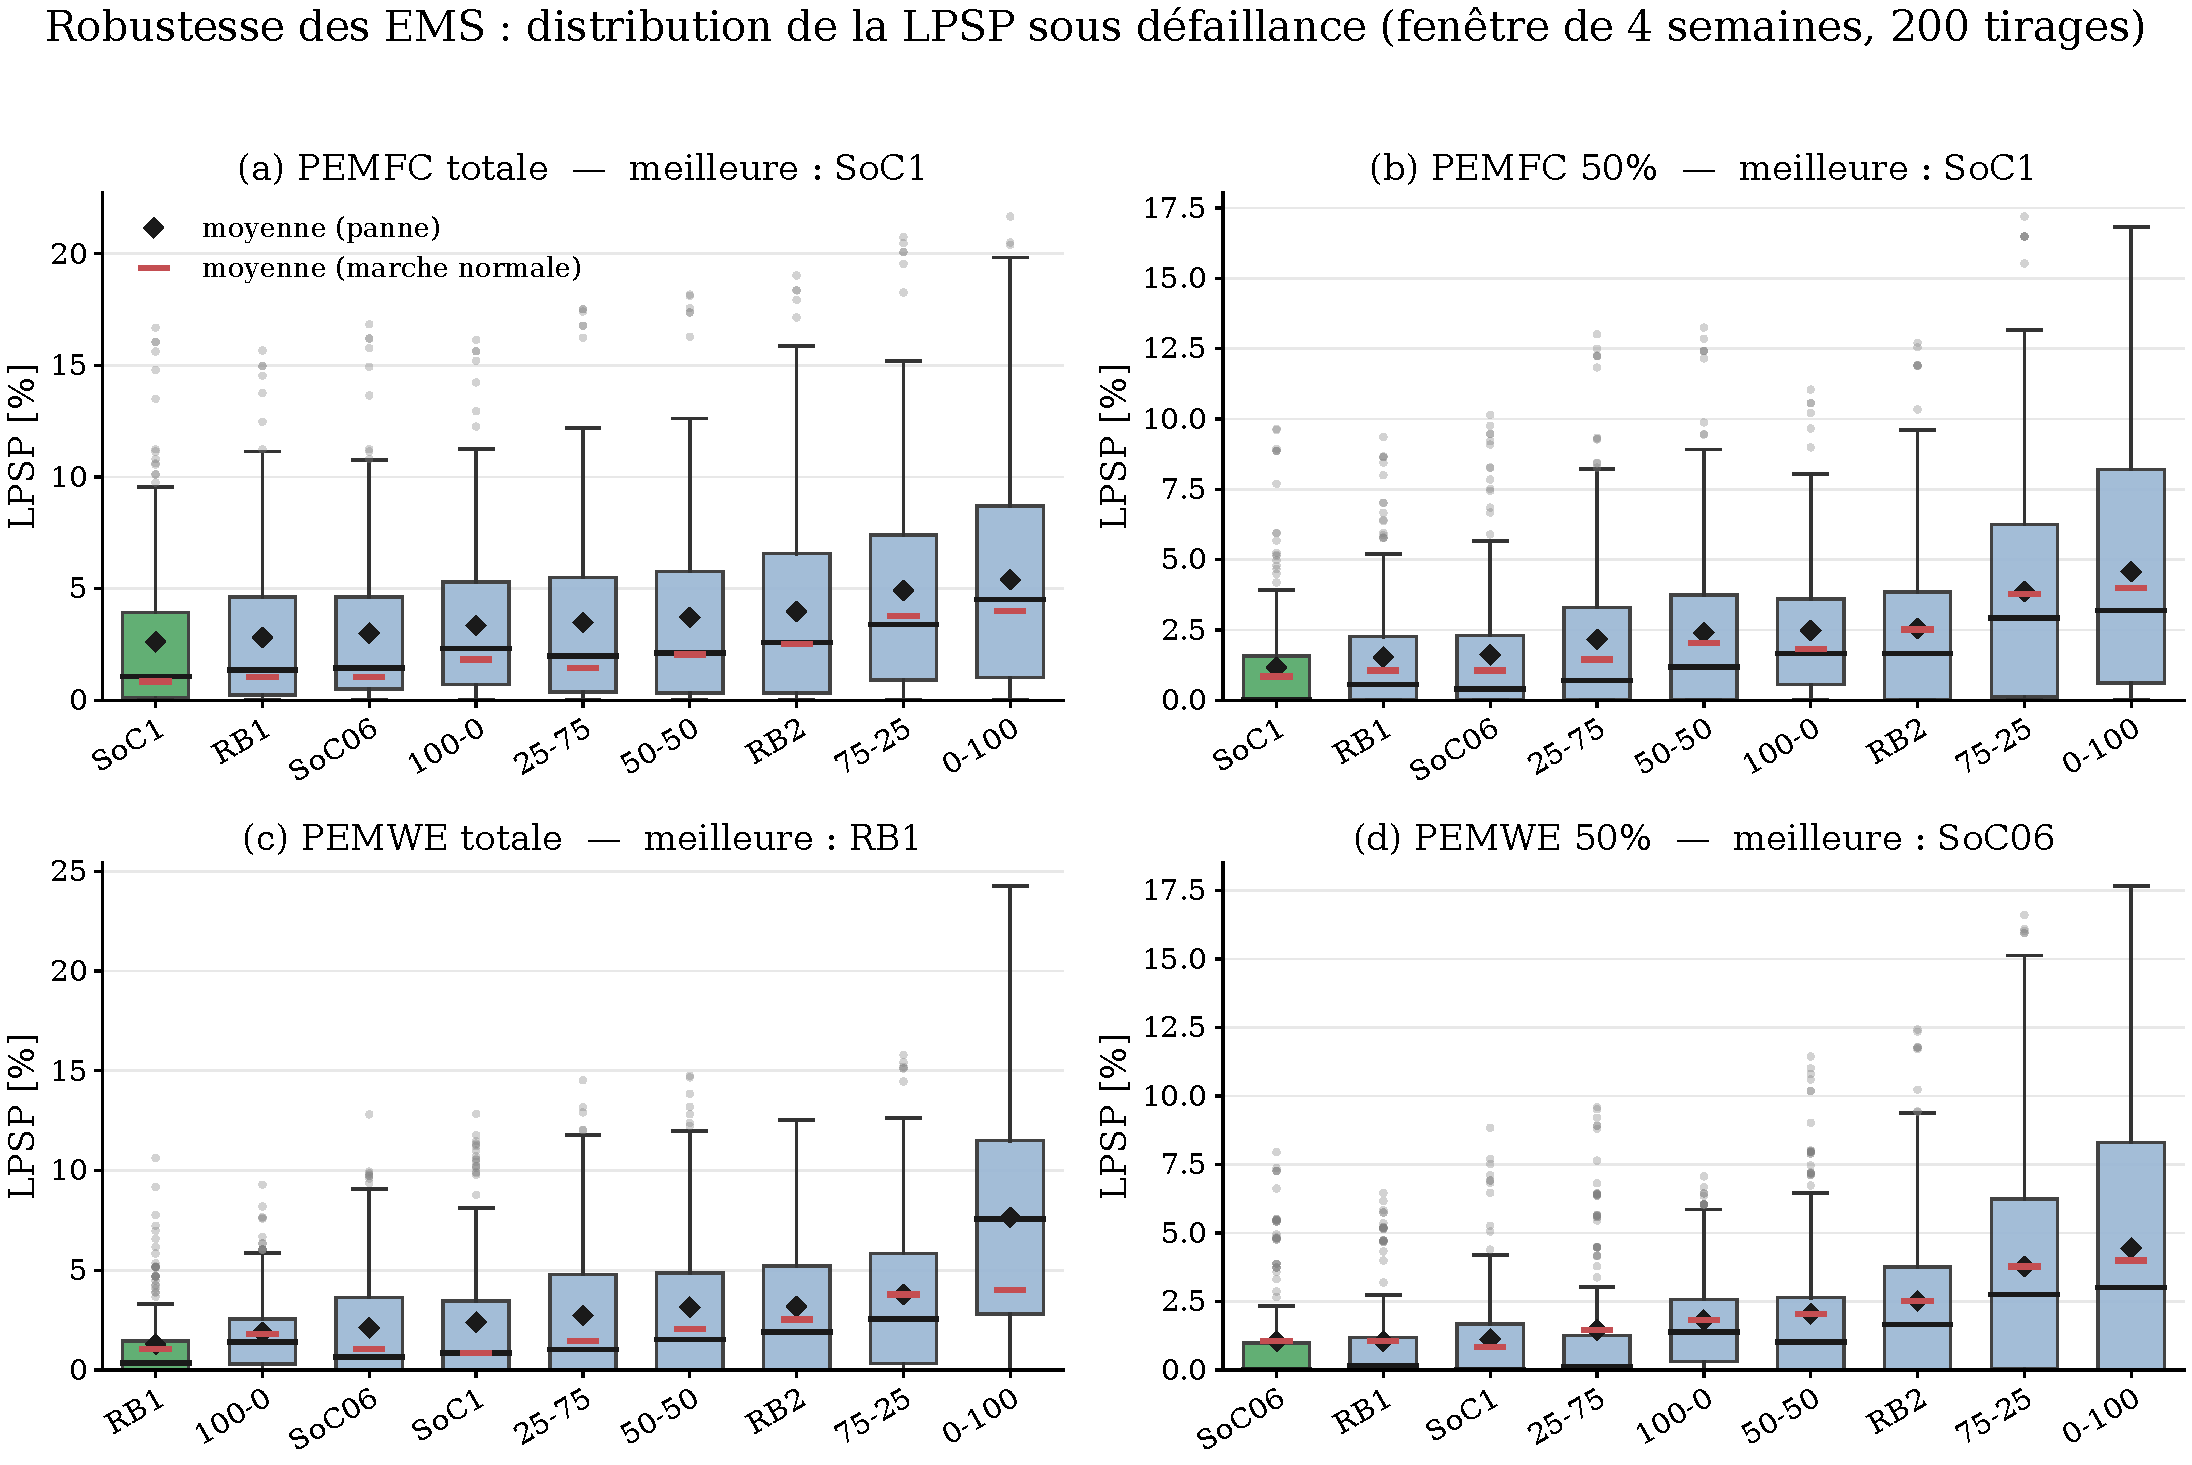
\includegraphics[width=\linewidth]{Chapitre 2/Robustesse/Figures/robustesse_boxplots.pdf}
    \caption{Distribution de la LPSP sous défaillance, par stratégie et par scénario (fenêtre de 4~semaines, 200~tirages).}
    \label{fig:rob_boxplots}
\end{figure}
\FloatBarrier

\begin{figure}[h!]
    \centering
    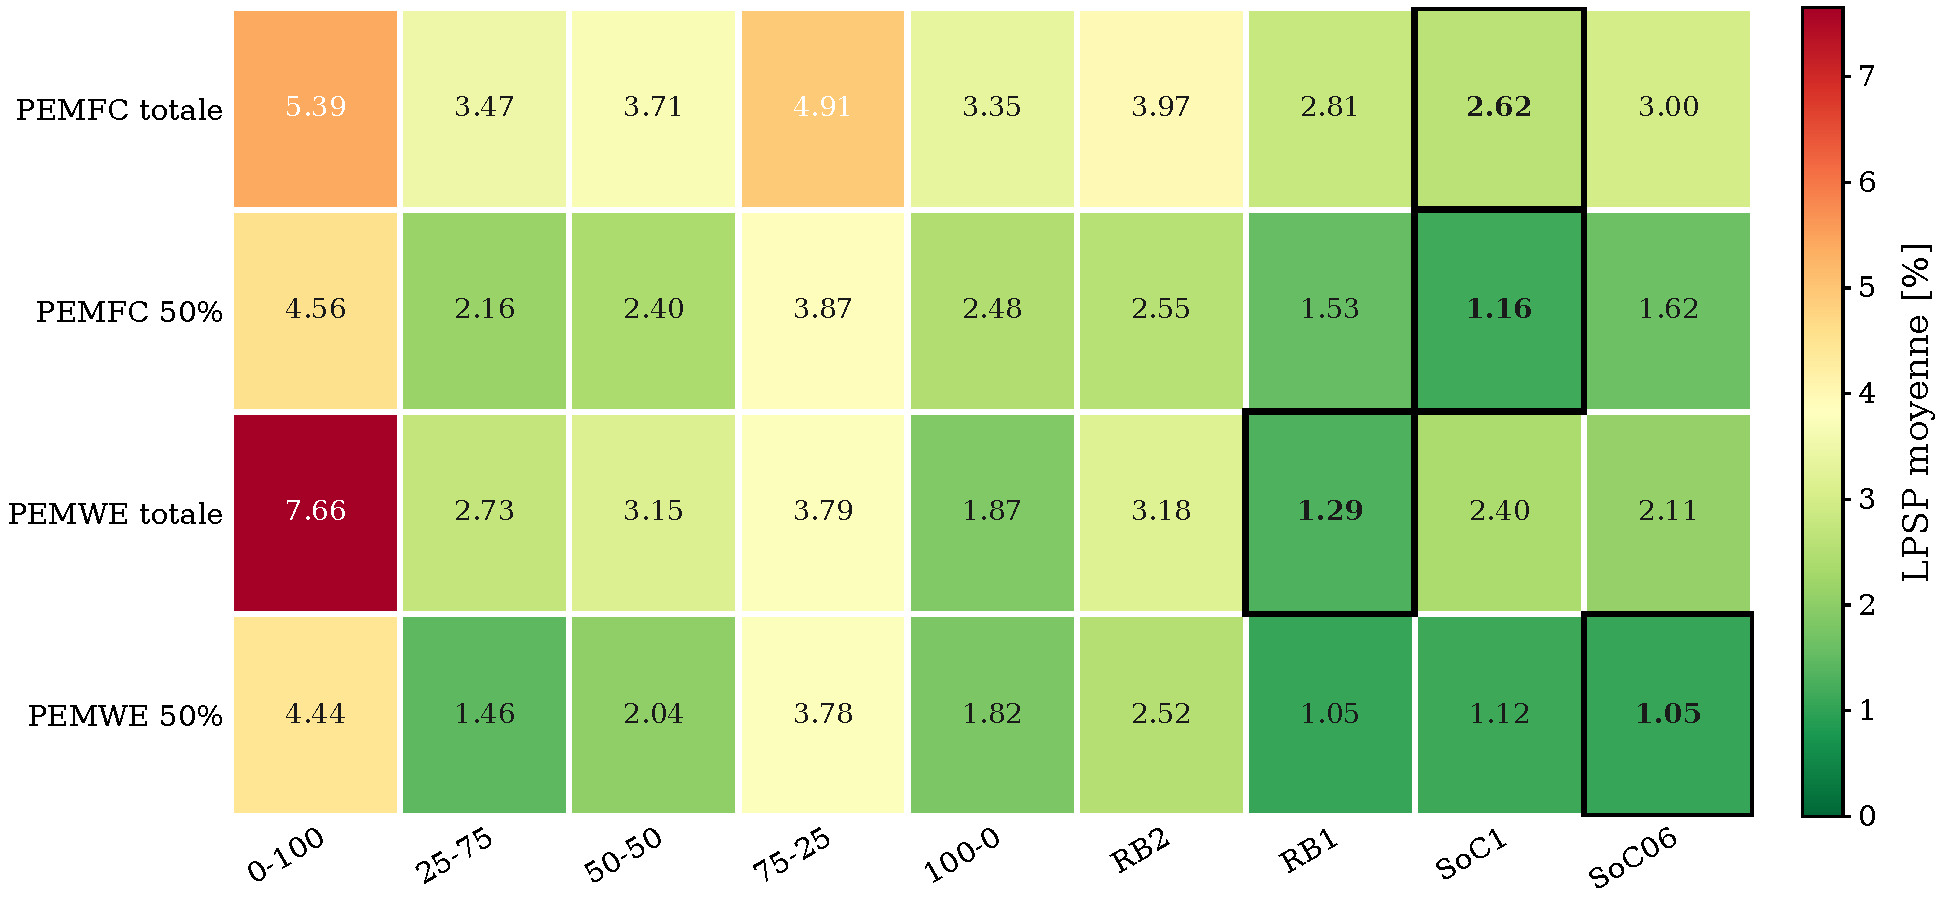
\includegraphics[width=\linewidth]{Chapitre 2/Robustesse/Figures/robustesse_heatmap.pdf}
    \caption{LPSP moyenne sous défaillance (scénario $\times$ stratégie). La cellule la plus favorable de chaque ligne est encadrée.}
    \label{fig:rob_heatmap}
\end{figure}
\FloatBarrier

\begin{figure}[h!]
    \centering
    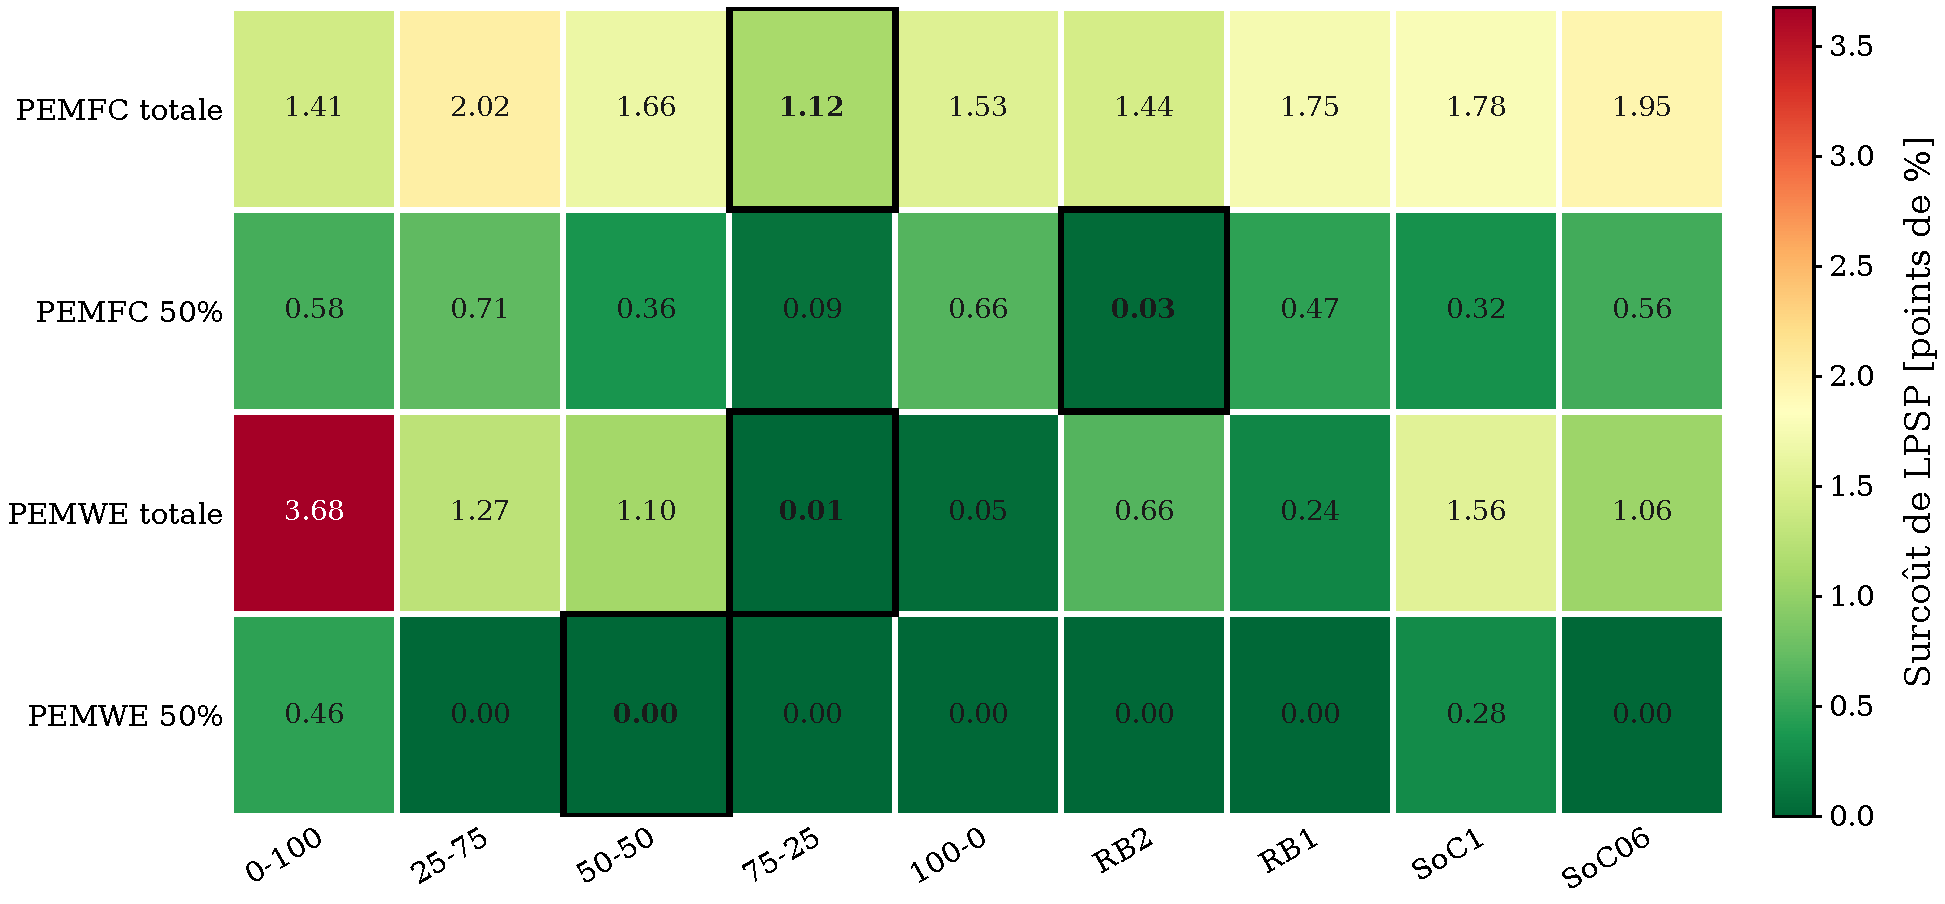
\includegraphics[width=\linewidth]{Chapitre 2/Robustesse/Figures/robustesse_heatmap_delta.pdf}
    \caption{Surcoût de défaillance $\Delta\mathrm{LPSP}_{\text{rob}} = \mathrm{LPSP}(\text{panne}) - \mathrm{LPSP}(\text{marche normale})$, en points de pourcentage.}
    \label{fig:rob_heatmap_delta}
\end{figure}
\FloatBarrier

En LPSP absolue (Figure~\ref{fig:rob_heatmap}), les stratégies maintenant une forte réserve de batterie s'en sortent le mieux. SoC1 minimise la LPSP en cas de défaillance de la pile à combustible (\SI{2{,}62}{\percent} en panne totale, \SI{1{,}16}{\percent} en panne partielle), tandis que RB1 et SoC06 dominent en cas de défaillance de l'électrolyseur (respectivement \SI{1{,}29}{\percent} pour la PEMWE totale et \SI{1{,}05}{\percent} pour la PEMWE \SI{50}{\percent}). Ce résultat est en partie trompeur, car ces stratégies présentent déjà une faible LPSP nominale (forte réserve d'énergie disponible)~: leur bonne tenue en panne reflète davantage leur fonctionnement de base que leur réaction propre à la défaillance.

Une fois isolé l'effet propre de la panne (Figure~\ref{fig:rob_heatmap_delta}), le classement change. Les stratégies à dominante batterie (75-25, 100-0, RB2) affichent les surcoûts les plus faibles, inférieurs à un dixième de point pour la défaillance partielle de la pile à combustible. À l'inverse, la stratégie « tout-hydrogène » 0-100 se dégrade fortement dès qu'un composant hydrogène défaille~: son surcoût atteint \SI{3{,}66}{} points en cas de panne totale de l'électrolyseur (LPSP moyenne de \SI{7{,}65}{\percent}, soit le pire cas observé), ce qui traduit une dépendance excessive au sous-système hydrogène et une absence de marge de repli. La défaillance partielle de l'électrolyseur (PEMWE \SI{50}{\percent}) engendre quant à elle des surcoûts quasi nuls pour la plupart des stratégies, le surplus PV non absorbé étant simplement réorienté vers la batterie, sans perte de service immédiate.

Le meilleur choix dépend donc du scénario considéré~: une défaillance de la pile à combustible est le mieux encaissée par les stratégies maintenant une forte réserve de batterie (SoC1), tandis qu'une défaillance de l'électrolyseur l'est par celles qui préservent une marge de charge (RB1, SoC06). Aucune stratégie ne minimise la LPSP dans tous les scénarios à la fois~: ce qui distingue les stratégies, c'est le composant dont elles dépendent et la marge de repli qu'elles conservent.

La LPSP moyenne ne dit rien de la dispersion des situations selon l'instant de la panne. Or, pour un système isolé, ce sont souvent les pires cas qui dimensionnent l'acceptabilité du service. La Figure~\ref{fig:rob_cdf} présente, pour chaque scénario, les fonctions de répartition de la LPSP sous défaillance. Leur lecture confirme et précise les conclusions précédentes~: les stratégies préservant une réserve de batterie présentent non seulement une LPSP moyenne plus faible, mais aussi des queues de distribution nettement plus courtes, c'est-à-dire des coupures maximales bien moindres lorsque la panne tombe au plus mauvais moment. À l'inverse, la courbe de l'EMS 0-100 s'étire loin vers la droite, traduisant des épisodes de coupure sévères (jusqu'à plus de \SI{24}{\percent} de LPSP sur la fenêtre en cas de panne totale de l'électrolyseur).

\begin{figure}[h!]
    \centering
    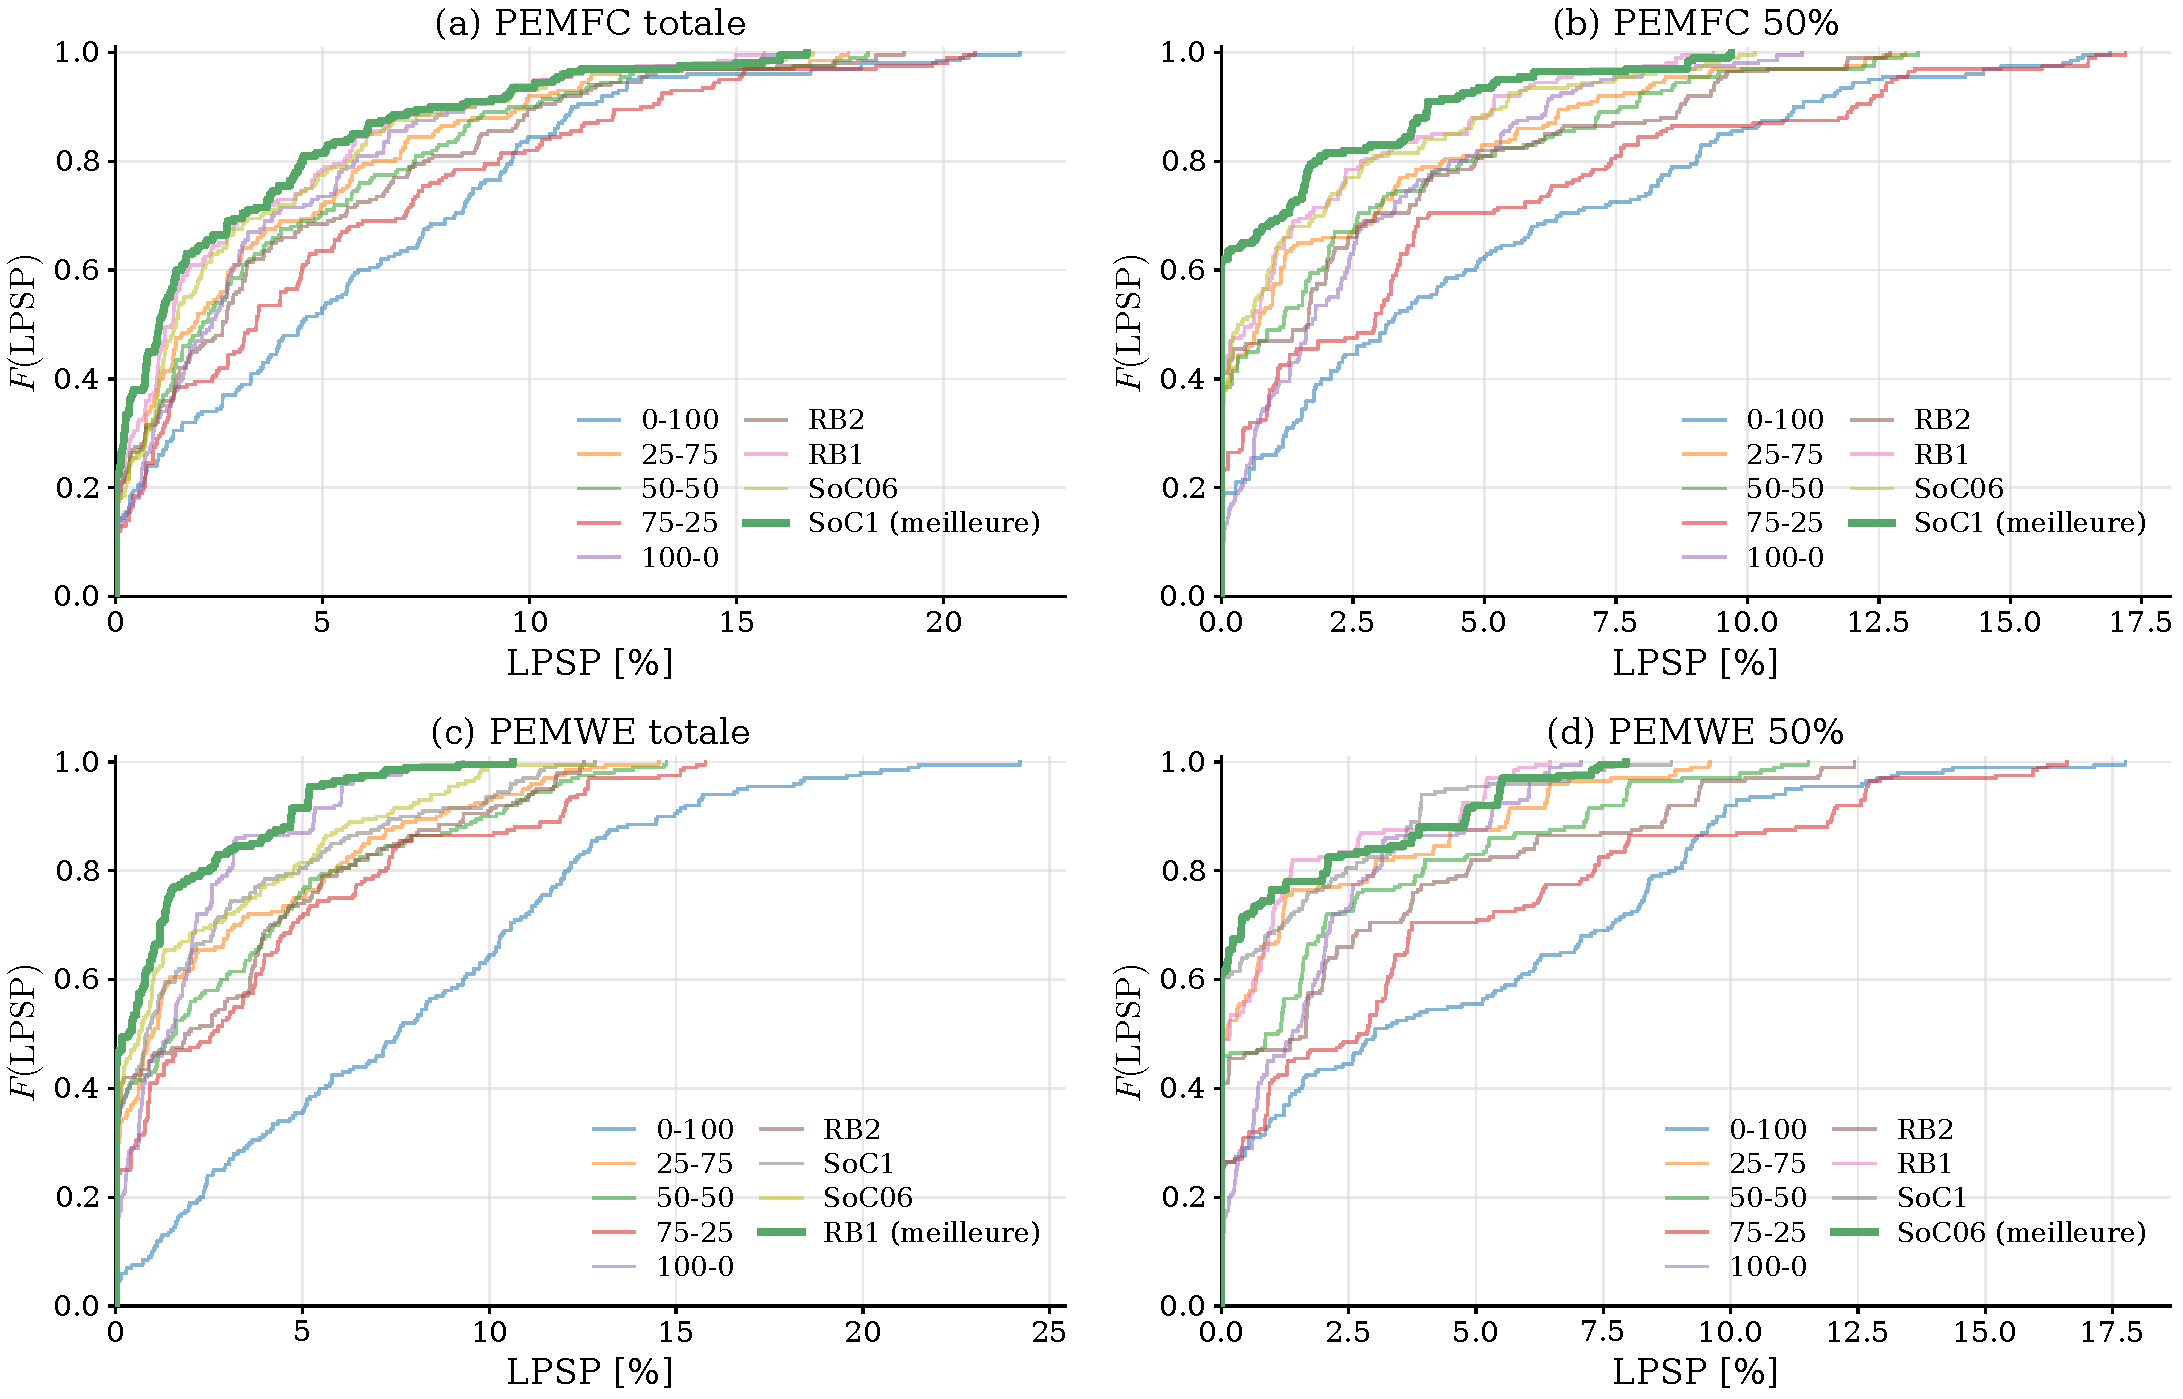
\includegraphics[width=\linewidth]{Chapitre 2/Robustesse/Figures/robustesse_cdf.pdf}
    \caption{Fonctions de répartition de la LPSP sous défaillance, par scénario.}
    \label{fig:rob_cdf}
\end{figure}
\FloatBarrier

% ------------------------------------------------------------
\subsubsection{Discussion}
% ------------------------------------------------------------

Le principal enseignement de cette analyse est qu'aucune stratégie ne domine simultanément les trois axes de performance. Les stratégies les plus robustes en LPSP absolue (SoC1, RB1) sont aussi parmi les plus coûteuses en dégradation, SoC1 culminant à 141~k€ sur le plan de Pareto, précisément parce que la forte réserve d'énergie qui les protège des pannes est obtenue au prix d'une sollicitation intense des composants hydrogène. Réciproquement, la stratégie 0-100, qui n'est pas la plus mauvaise sur le plan de Pareto nominal, se révèle la plus fragile face aux défaillances. La robustesse constitue donc une dimension de performance distincte, non réductible au compromis entre LPSP et dégradation, et qui mérite d'être évaluée explicitement.

La lecture des quatre scénarios met par ailleurs en évidence une asymétrie entre les deux composants hydrogène et entre les deux sévérités. La défaillance de la pile à combustible se traduit immédiatement par un déficit de service~: la PAC étant le seul organe capable de restituer l'énergie stockée sous forme d'hydrogène en période de déficit, sa perte ne peut être compensée que par la batterie, dont la réserve devient alors déterminante. La défaillance de l'électrolyseur n'a en revanche pas d'effet immédiat sur la satisfaction de la charge~: le surplus PV qui ne peut plus être électrolysé est simplement réorienté vers la batterie ou écrêté, sans coupure. Son coût est différé~: faute de pouvoir reconstituer le stock d'hydrogène pendant la panne, le réservoir s'appauvrit et la pile à combustible finit par manquer de carburant. C'est pourquoi la LPSP est évaluée sur une fenêtre incluant la reprise post-réparation, comme discuté à la section~\ref{subsec:indic_robustesse}. Les défaillances partielles (\SI{50}{\percent}) sont quant à elles bien mieux encaissées que les pannes totales~: la capacité résiduelle suffit souvent à couvrir une part substantielle de la demande, ce qui ramène le surcoût à des valeurs faibles voire négligeables, en particulier pour l'électrolyseur.

Les surcoûts très faibles relevés pour les défaillances partielles, en particulier celle de l'électrolyseur, pourraient laisser croire à un surdimensionnement des composants. Cette lecture serait toutefois trompeuse. Un électrolyseur dimensionné, par exemple, moitié plus petit ne dégraderait pas nécessairement la LPSP (sa capacité résiduelle resterait souvent suffisante pour absorber le surplus photovoltaïque), mais il fonctionnerait en permanence à une puissance relative bien plus élevée, et serait donc davantage exposé aux mécanismes d'usure liés au fonctionnement soutenu à forte charge. La bonne tenue apparente sous défaillance partielle ne saurait donc justifier un sous-dimensionnement, qui se paierait en durabilité.

Sur le plan opérationnel, ces résultats convergent vers une recommandation simple~: une réserve de batterie suffisante constitue la principale marge de robustesse d'un tel système isolé. Les stratégies qui épuisent ou immobilisent cette réserve, en la maintenant artificiellement haute au prix d'une forte sollicitation hydrogène (SoC1) ou en s'en remettant presque exclusivement à l'hydrogène (0-100), sont les plus pénalisées lors d'une panne. Toute stratégie conservant une marge de batterie mobilisable transforme à l'inverse cette marge en assurance face aux défaillances. Ce constat plaide aussi, en pratique, pour un léger surdimensionnement de la batterie et pour une maintenance préventive ciblant en priorité la pile à combustible, dont la défaillance est la plus immédiatement pénalisante.

Un autre point central mérite d'être souligné~: les défaillances considérées sont supposées mesurables, c'est-à-dire détectées par la supervision dès leur apparition. Cette hypothèse est raisonnable pour des composants instrumentés, dont la mise hors service ou le dérating est directement observable. Rien n'oblige alors à conserver, pendant la panne, la stratégie employée en régime nominal. Dès qu'une défaillance est détectée, la supervision peut basculer, le temps de l'indisponibilité, vers la stratégie qui minimise la LPSP dans le scénario rencontré (Figure~\ref{fig:rob_heatmap}), avant de revenir au régime nominal après réparation. L'analyse de robustesse ne désigne donc pas une stratégie unique~: elle fournit, pour chaque type de panne, la stratégie de repli la plus appropriée. Ces résultats ne remettent pas en cause le choix de la stratégie nominale issu du plan de Pareto, qui demeure de mise en fonctionnement normal et servira de point de départ à l'approche anticipative du chapitre suivant~; ils le complètent d'une politique de repli activée à la détection d'une panne.

Cette étude appelle néanmoins quelques réserves méthodologiques. La panne est ici supposée parfaitement détectée et instantanément prise en compte par le répartiteur~; un retard de détection ou un diagnostic erroné dégraderait les performances, en particulier pour les stratégies les plus dépendantes du composant défaillant. Par ailleurs, seules les défaillances des composants hydrogène ont été considérées et la durée de panne a été fixée à une semaine~; l'extension à des défaillances de batterie, à des durées variables ou à des pannes simultanées constitue une perspective naturelle. Enfin, la robustesse a été évaluée à travers la seule LPSP~; elle pourrait être complétée par un coût de la charge non desservie, dans l'esprit du critère de coût total unifié introduit à la section suivante.

% ============================================================
%  CHAPITRE 2 — Section : Analyse de sensibilité & coût total unifié (VoLL)
% ============================================================

\section{Analyse de sensibilité \& coût total unifié}
\label{sec:sensibilite}

L'ensemble des résultats présentés jusqu'ici découle d'une simulation déterministe unique, conduite avec des paramètres nominaux. La pertinence du classement des stratégies, et en particulier le statut de meilleure stratégie statique attribué à RB2, doit donc être confrontée à l'incertitude qui entache les principales hypothèses de modélisation. Cette section répond à cette exigence en plusieurs temps~: deux vérifications spécifiques (robustesse au bruit d'estimation du SoH, puis sensibilité à la résolution temporelle), une analyse de sensibilité de Monte-Carlo appliquée uniformément à l'ensemble des EMS, et enfin la réduction des deux objectifs à un \emph{coût total unifié} reposant sur une valeur de la charge non desservie, qui permet de classer les stratégies par un critère scalaire unique.

% ------------------------------------------------------------
\subsection{Robustesse de l'approche réactive au bruit d'estimation}
% ------------------------------------------------------------

Une première vérification concerne spécifiquement l'approche réactive au vieillissement, commune à toutes les EMS~: celle-ci agit sur le SoH \emph{estimé}, et non sur sa valeur réelle. Pour s'assurer que cette dépendance ne constitue pas une fragilité, un bruit d'estimation gaussien d'écart-type \SI{2}{\percent}, rafraîchi chaque semaine, est injecté sur l'estimation du SoH utilisée pour actualiser les plages de fonctionnement. Les performances restent alors très proches du cas à information exacte~: l'actualisation réactive des limites physiques se révèle essentiellement insensible à un bruit d'estimation réaliste, et le classement des stratégies n'en est pas affecté. Ce résultat conforte l'hypothèse, posée à la section~\ref{sec:soh}, selon laquelle les méthodes d'estimation existantes sont suffisamment précises pour les besoins du contrôle.

% ------------------------------------------------------------
\subsection{Sensibilité à la résolution temporelle}
% ------------------------------------------------------------

Une seconde vérification porte sur le pas d'échantillonnage. Toutes les simulations précédentes ont été conduites à pas horaire, qui néglige par construction les variations infra-horaires de la production PV et de la demande, et donc une partie des sollicitations rapides des composants. Pour éprouver ce choix, la stratégie de référence RB2 est resimulée sur l'horizon complet à un pas de \SI{10}{\minute}, en injectant sur les profils PV et de charge un bruit gaussien intra-horaire d'écart-type $\sigma \in \{0,5,10,15\}\,\%$ de la valeur horaire, la moyenne horaire étant préservée de sorte que le bilan énergétique et les décisions de l'EMS restent inchangés.

Sans bruit, la simulation à \SI{10}{\minute} reproduit fidèlement la simulation horaire (coût de dégradation $65{,}4 \rightarrow 65{,}9$~k€, LPSP $\approx \SI{2{,}45}{\percent}$). La restitution des variations intra-horaires accroît en revanche le coût de dégradation de façon monotone avec l'amplitude du bruit, jusqu'à environ $+\SI{15}{\percent}$ à $\sigma = \SI{15}{\percent}$ ($65{,}4 \rightarrow 75{,}2$~k€)~: la résolution horaire sous-estime donc légèrement la dégradation. La LPSP reste quant à elle quasiment inchangée ($\approx \SI{2{,}45}{\percent}$), et la hiérarchie des mécanismes de dégradation (en particulier la prééminence des cycles de démarrage-arrêt) est préservée à tous les pas et amplitudes. Le pas horaire constitue ainsi une estimation \emph{conservatrice} (borne inférieure) de la dégradation, sans remettre en cause les conclusions tirées du classement des stratégies.

% ------------------------------------------------------------
\subsection{Analyse de sensibilité de Monte-Carlo}
% ------------------------------------------------------------

Au-delà de cette vérification spécifique, les incertitudes de modélisation restantes affectent toutes les stratégies de la même manière~; elles sont donc évaluées par des analyses de sensibilité de Monte-Carlo appliquées uniformément à l'ensemble des EMS. Quatre familles d'incertitude sont considérées~:
\begin{itemize}
  \setlength\itemsep{2pt}
  \item les \textbf{critères de fin de vie} (EoL) des trois composants~: SoH de fin de vie de la batterie tiré dans $[0{,}60\,;\,0{,}80]$, et des composants hydrogène dans $[0{,}85\,;\,0{,}95]$~;
  \item les \textbf{seuils de la fonction de dégradation} des composants hydrogène, c'est-à-dire les seuils de régime du modèle de dégradation par morceaux, chacun échantillonné à $\pm\SI{20}{\percent}$ de sa valeur nominale~;
  \item les \textbf{poids de coût de remplacement} qui pondèrent la contribution de chaque composant à l'axe des coûts, chacun varié de $\pm\SI{30}{\percent}$ (la LPSP étant invariante à ces poids, cet échantillonnage se réduit à une dilatation analytique de l'axe des coûts)~;
  \item le \textbf{dimensionnement des composants}, les puissances/capacités de la batterie, de la pile à combustible et de l'électrolyseur étant chacune multipliées par un facteur indépendant tiré uniformément dans $[0{,}80\,;\,1{,}20]$, le champ PV étant laissé inchangé.
\end{itemize}
Chaque famille repose sur $N = 200$ tirages, les mêmes étant réutilisés pour toutes les stratégies afin que la comparaison ne soit pas polluée par le bruit d'échantillonnage. Chaque tirage est propagé à travers une simulation complète de vingt-cinq ans, fournissant pour chaque stratégie un résultat bidimensionnel (LPSP et coût de dégradation). Le Tableau~\ref{tab:sensitivity} en résume les plages et les conclusions, et la Figure~\ref{fig:sens_eol} en illustre un exemple (échantillonnage des critères de fin de vie) sous forme de nuage de points dans le plan de Pareto, assorti d'ellipses de dispersion.

\begin{table}[h!]
\centering
\caption{Analyses de sensibilité~: plages de perturbation et conclusions. Le classement des stratégies est préservé dans tous les cas.}
\label{tab:sensitivity}
\footnotesize
\renewcommand{\arraystretch}{1.25}
\begin{tabularx}{\textwidth}{p{3.3cm} X X}
\hline
\textbf{Analyse} & \textbf{Paramètre(s) et plage} & \textbf{Conclusion} \\ \hline
Erreur d'estimation du SoH & Bruit gaussien $\sigma = \SI{2}{\percent}$, rafraîchi chaque semaine & Performances quasi inchangées~; classement préservé. \\
Poids de coût & $\pm\SI{30}{\percent}$ sur les trois poids de remplacement & LPSP invariante~; coût linéaire en les poids~; classement inchangé (coût RB2 $65{,}6$~k€, IC~95\,\% $[51{,}3\,;\,80{,}0]$). \\
Critères de fin de vie & Batterie $[0{,}60\,;\,0{,}80]$, PAC/ELY $[0{,}85\,;\,0{,}95]$ & Effet marqué sur le coût absolu (durée de vie batterie $5{,}5 \rightarrow 2{,}5$~ans) mais classement inchangé (coût RB2 $62{,}6 \pm 9{,}5$~k€). \\
Seuils de dégradation PEM & Les quatre seuils de régime, chacun $\pm\SI{20}{\percent}$ & Classement inchangé~; coût RB2 $65{,}4 \rightarrow 66{,}9 \pm 9{,}7$~k€. \\
Dimensionnement & Calibres BAT/PAC/ELY $\times[0{,}80\,;\,1{,}20]$, PV fixe & Les deux axes se déplacent (batterie plus grande $\rightarrow$ LPSP plus faible, coût plus élevé) mais classement inchangé~; RB2 reste favorable (dég. $64{,}6 \pm 4{,}2$~k€, LPSP $3{,}06 \pm 0{,}79\,\%$). \\
Résolution temporelle & $T_s = \SI{10}{\minute}$ vs $\SI{1}{\hour}$~; bruit gaussien intra-horaire sur PV \& charge, $\sigma \in \{0,5,10,15\}\,\%$ (moyenne horaire préservée) & Seul le coût de dégradation croît avec le bruit (RB2 $65{,}4 \rightarrow 75{,}2$~k€)~; LPSP $\approx \SI{2{,}45}{\percent}$ et hiérarchie des mécanismes inchangées. \\ \hline
\end{tabularx}
\end{table}
\FloatBarrier

\begin{figure}[h!]
    \centering
    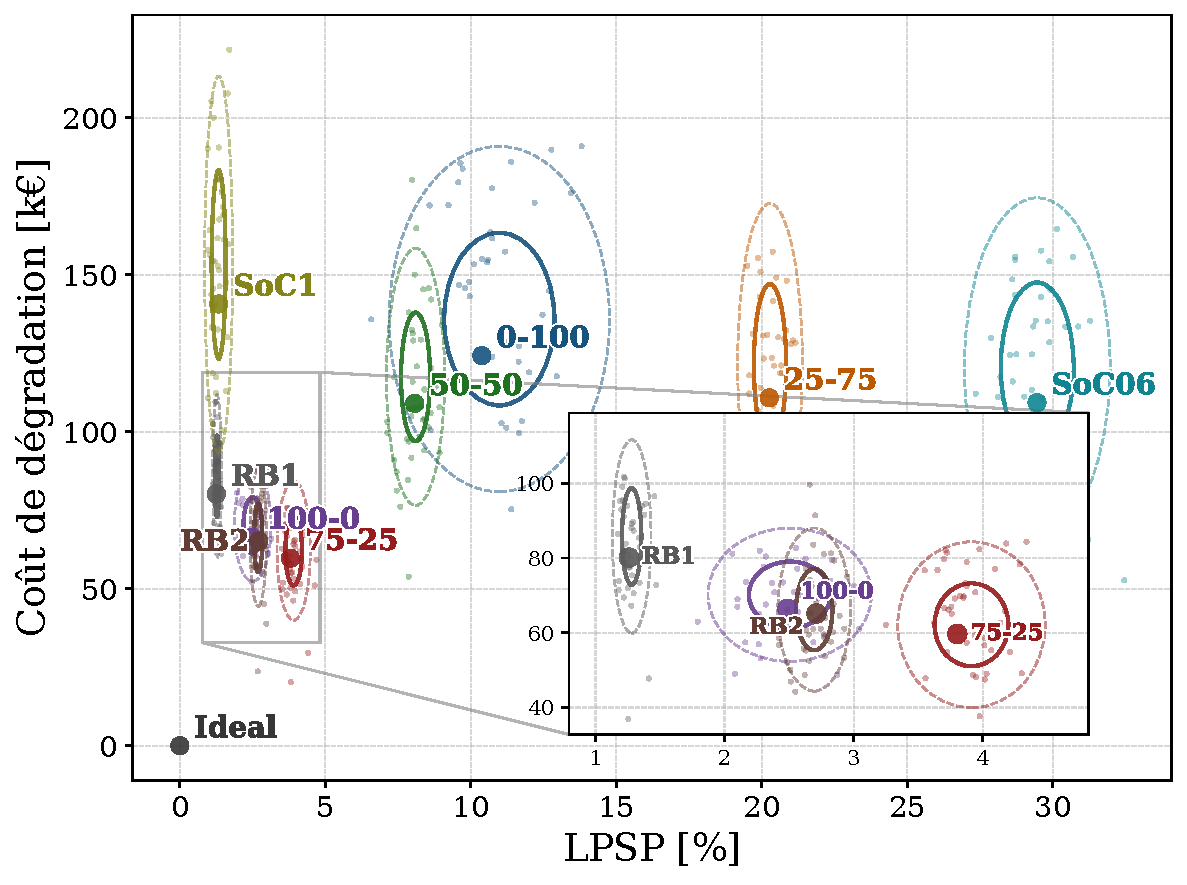
\includegraphics[width=0.8\linewidth]{Chapitre 2/Sensibilite/Figures/sens_eol_pareto.pdf}
    \caption{Plan de Pareto sous échantillonnage de Monte-Carlo des critères de fin de vie (ellipses de dispersion à $1\sigma$ en trait plein et $2\sigma$ en pointillés).}
    \label{fig:sens_eol}
\end{figure}
\FloatBarrier

Deux conclusions robustes se dégagent. Premièrement, chaque perturbation se contente, pour l'essentiel, de \emph{redimensionner} les indicateurs absolus sans rebattre l'ordre des stratégies~: les perturbations de poids et de seuils dilatent principalement l'axe des coûts, les critères de fin de vie en déplacent en outre le niveau absolu (la durée de vie de la batterie variant de $5{,}5$ à $2{,}5$~ans), et la perturbation de dimensionnement déplace les deux axes (une batterie plus grande abaissant la LPSP au prix d'un coût de dégradation supérieur). Dans tous les cas, RB2 conserve sa position favorable et non dominée. Le cas du dimensionnement mérite un commentaire spécifique~: la configuration nominale (un champ PV surdimensionné par rapport à la charge, d'où un électrolyseur surdimensionné et une pile à combustible sous-dimensionnée) découle directement des profils de terrain du cas d'étude~; la perturbation de $\pm\SI{20}{\percent}$ confirme que le classement reflète la logique de contrôle et non ce point de dimensionnement particulier.

% ------------------------------------------------------------
\subsection{Critère de coût total unifié (VoLL)}
% ------------------------------------------------------------

Comparer les stratégies sur chaque plan de Pareto bidimensionnel est instructif mais fastidieux, d'autant que les deux objectifs sont exprimés dans des unités différentes (un pourcentage et un coût). Un critère plus concis et plus directement objectivable consiste à réduire le résultat à un scalaire unique, en attribuant une valeur monétaire à la charge non desservie au moyen d'une \emph{valeur de la charge perdue} (VoLL, \textit{Value of Lost Load}), ajoutée au coût de dégradation~\cite{keskinis_techno-economic_2025}~:
\begin{equation}
    C_{\text{tot}} = C_{\text{deg}} + \mathrm{VoLL} \times E_{\text{non servie}}
    \label{eq:total_cost}
\end{equation}
où $E_{\text{non servie}} = \mathrm{LPSP} \times E_{\text{planifiée}}$ est l'énergie que les usagers prévoyaient de consommer mais que le système n'a pu fournir sur l'ensemble de l'horizon, $E_{\text{planifiée}}$ étant l'énergie de charge nette planifiée et LPSP la probabilité de perte d'alimentation. Conformément à la pratique courante en évaluation de fiabilité des micro-réseaux, la VoLL est maintenue constante et fixée à $\mathrm{VoLL} = 3~\text{€/kWh}$, valeur médiane représentative d'une charge résidentielle mixte~\cite{CEPA2018VoLL}\cite{jin_evaluating_2025}. Ce choix conditionne l'arbitrage entre les deux objectifs~: une VoLL faible privilégie les stratégies sobres en dégradation, tandis qu'une VoLL élevée favoriserait celles qui minimisent la LPSP (RB1, SoC1). Pour la valeur retenue, intermédiaire, le classement reste stable et RB2 conserve sa position de tête (Fig. \ref{fig:ranking}). Le scalaire unique $C_{\text{tot}}$ rend les stratégies directement comparables, aussi bien à l'intérieur de chaque cas de sensibilité qu'entre les différents cas.

La réduction de chaque résultat au scalaire $C_{\text{tot}}$ produit le classement unifié de la Figure~\ref{fig:ranking}. RB2 obtient le \textbf{meilleur rang moyen} ($1{,}2$ sur l'ensemble des cas) et se classe première dans quatre des cinq cas de sensibilité (nominal, critères de fin de vie, poids de coût et dimensionnement). Elle n'est devancée que sur le seul cas des seuils de dégradation des composants hydrogène, où la stratégie « tout-batterie » 100-0 réalise le coût total le plus faible. Ces deux stratégies sont d'ailleurs très rapprochées (rang moyen $1{,}2$ pour RB2 contre $1{,}8$ pour 100-0) et devancent nettement les suivantes (RB1 puis 75-25), tandis que les stratégies très coûteuses en dégradation (SoC1) ou à forte LPSP (50-50, 0-100, 25-75 et surtout SoC06) ferment la marche dès lors que la charge non desservie est valorisée. RB2 demeure ainsi la stratégie la plus régulièrement performante, sans être strictement dominante~: ce point de vue scalaire confirme et nuance à la fois le verdict du plan de Pareto nominal. Il est à noter que ce constat est lui même dépendant de la valeur de VoLL fixée, et dans ce cas RB2 reste la stratégie la plus performante jusqu'à une valeur de 5,2€/kWh, au-delà de laquelle RB1 devient la stratégie la plus intéressante.

\begin{figure}[h!]
    \centering
    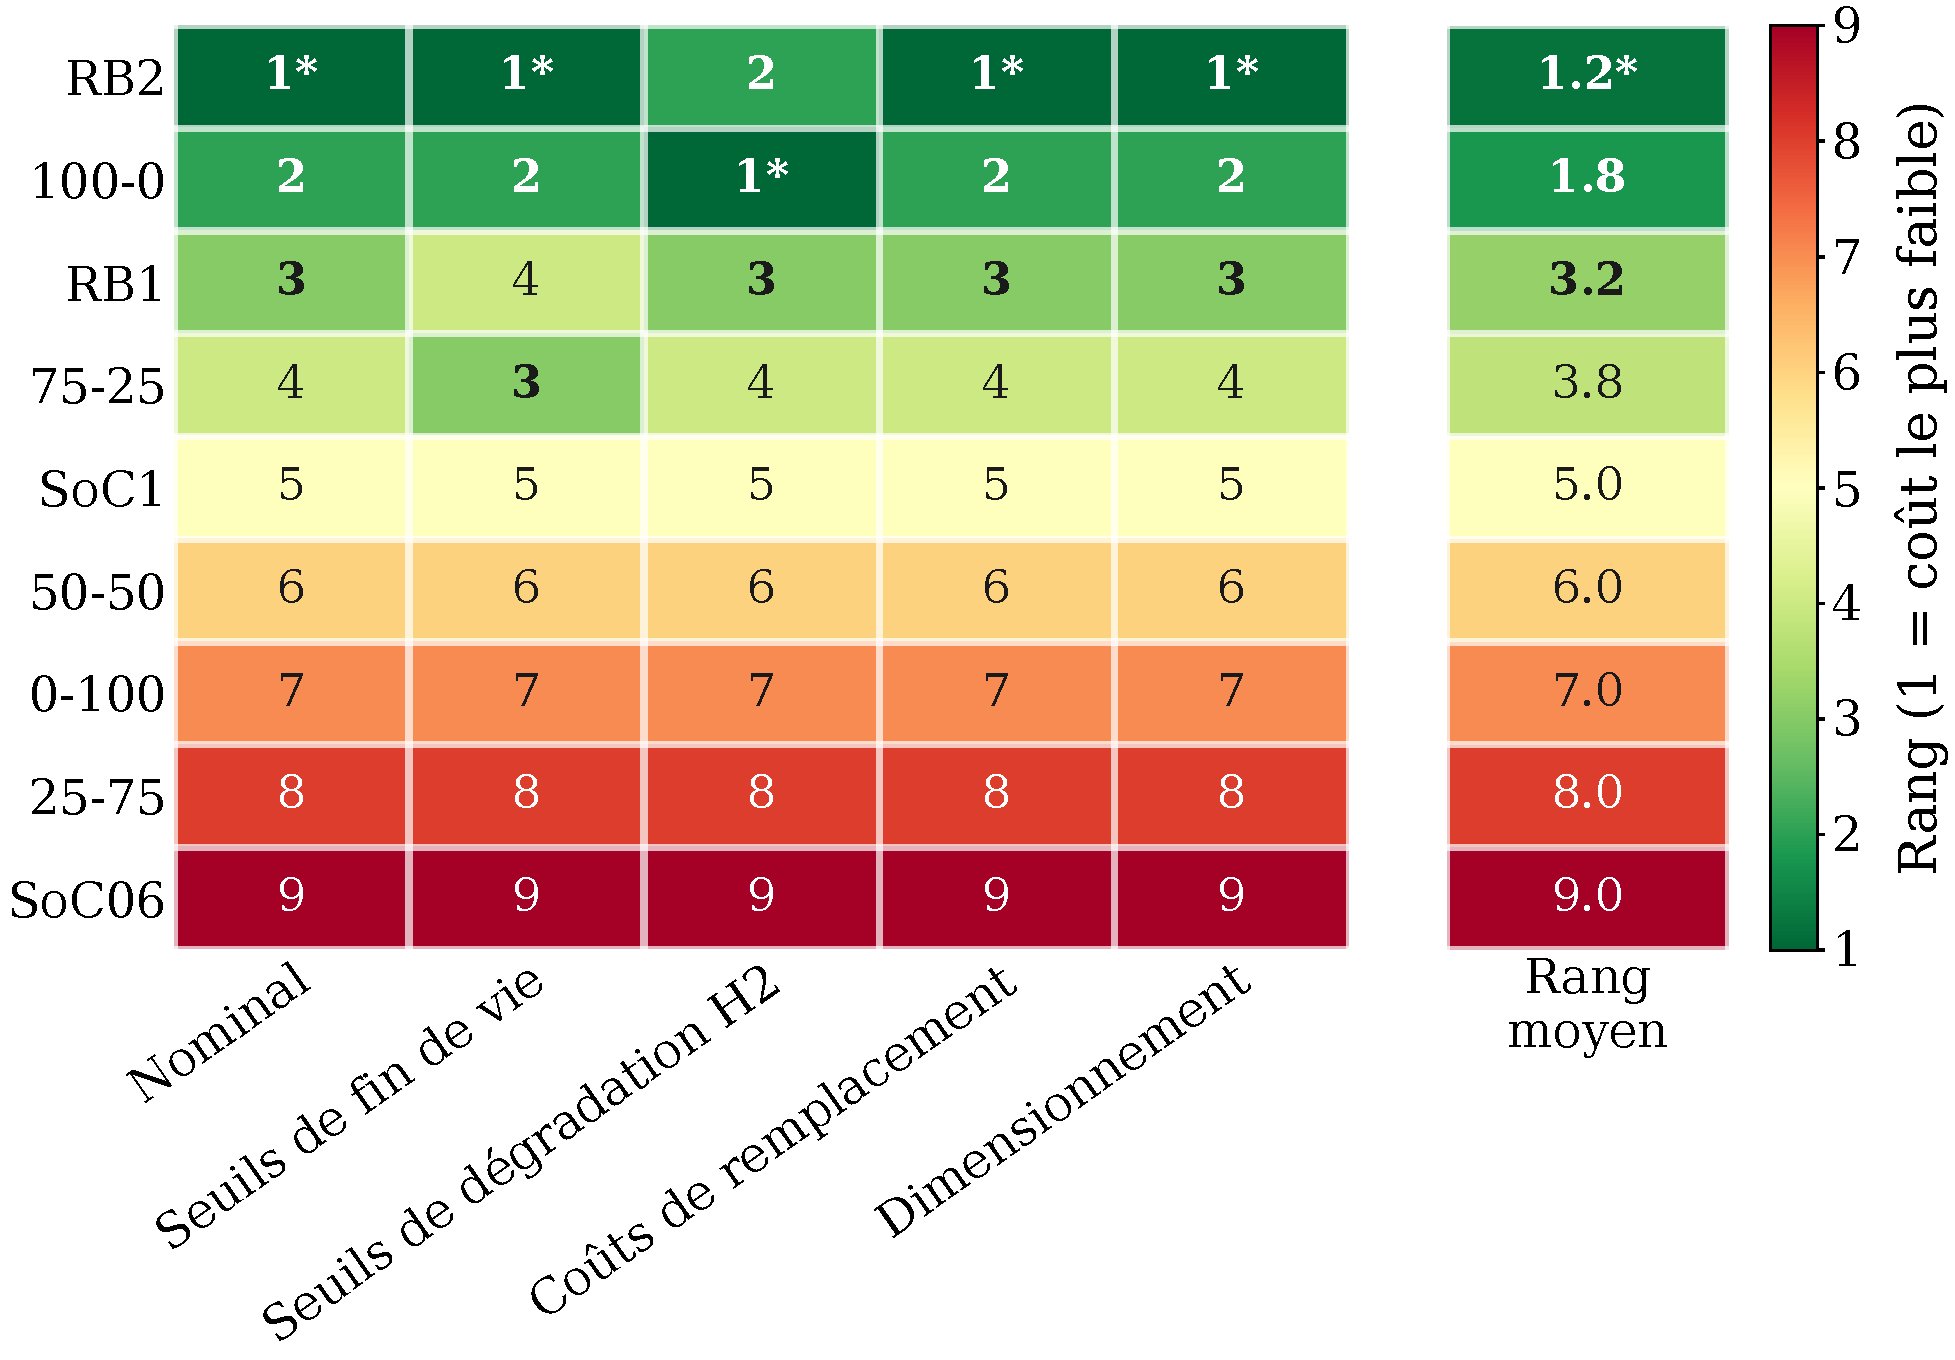
\includegraphics[width=\linewidth]{Chapitre 2/Sensibilite/Figures/voll_ranking_fr.pdf}
    \caption{Classement unifié par le coût total $C_{\text{tot}}$ à travers les cas de sensibilité.}
    \label{fig:ranking}
\end{figure}
\FloatBarrier

Au sens du coût total unifié, RB2 apparaît donc comme la stratégie statique la plus régulièrement performante, et ce de manière cohérente sur toute la gamme des hypothèses de modélisation et de dimensionnement testées. Ce constat consolide le choix de RB2 comme stratégie de référence et ouvre la voie à son amélioration au chapitre suivant.

% ============================================================
%  CHAPITRE 2 — Section : Bouclage avec le dimensionnement & conclusion
% ============================================================

\section{Limites \& conclusion du chapitre}
\label{sec:conclusion_chap}

% ============================================================
% [DÉSACTIVÉ] Bouclage avec le dimensionnement du micro-réseau.
% Mis en commentaire (cf. demande) ; à réactiver ultérieurement.
% ============================================================
\iffalse
% ------------------------------------------------------------
\subsection{Bouclage avec le dimensionnement du micro-réseau}
% ------------------------------------------------------------

L'ensemble des analyses de ce chapitre a été conduit à \emph{dimensionnement fixé}~: les calibres des composants ne varient pas d'une stratégie à l'autre, ce qui garantit que les écarts de performance observés sont uniquement imputables aux décisions de contrôle et non à des effets de dimensionnement. Ce choix méthodologique est essentiel pour une comparaison équitable des EMS, mais il appelle deux nuances.

D'une part, le dimensionnement retenu n'est pas issu d'une optimisation~: il a été calé grossièrement à partir des observations de terrain du cas d'étude de La Réunion. En particulier, le champ PV est largement surdimensionné relativement à la demande, ce qui entraîne un électrolyseur surdimensionné par rapport à la pile à combustible, et une capacité de stockage assurant plusieurs jours d'autonomie. Cette configuration n'est donc pas nécessairement optimale sur le plan technico-économique~; elle reflète une installation réelle.

D'autre part, et c'est le point important pour le bouclage, la robustesse du classement des stratégies vis-à-vis du dimensionnement a été explicitement évaluée à la section~\ref{sec:sensibilite}~: sous une perturbation de Monte-Carlo de $\pm\SI{20}{\percent}$ des calibres des composants, l'ordre des stratégies est préservé et RB2 conserve sa position de meilleure stratégie statique. Le classement obtenu reflète donc la logique de contrôle, et non le point de dimensionnement particulier du cas d'étude. Il n'en demeure pas moins qu'une \emph{co-optimisation conjointe} du dimensionnement et de la stratégie de gestion d'énergie apporterait un éclairage complémentaire sur la faisabilité pratique et le passage à l'échelle des EMS proposées. Cet aspect dépasse le cadre du présent chapitre~; il est étudié dans le cadre du projet ANR-22-CE05-0026, dont ces travaux font partie.
\fi

% ------------------------------------------------------------
\subsection{Limites de l'étude}
% ------------------------------------------------------------

Les résultats présentés doivent être tempérés par plusieurs limites inhérentes à la démarche. Premièrement, ils sont fortement liés aux profils de puissance utilisés, issus de données réelles reflétant les habitudes de consommation des populations locales~; ces profils ayant été construits pour refléter la réalité spécifique du cas d'étude, les conclusions chiffrées restent avant tout valables pour ce micro-réseau. Si les positions absolues dans le plan de Pareto sont spécifiques au climat et au dimensionnement (un site plus froid ou plus intermittent les déplacerait et appellerait un dimensionnement différent), la méthodologie proposée et le mécanisme qualitatif sous-jacent au classement des stratégies ont vocation à se transposer à d'autres contextes hors-réseau.

Deuxièmement, l'analyse a été menée à dimensionnement simplifié et fixé~; bien que la robustesse du classement à des variations de $\pm\SI{20}{\percent}$ des calibres ait été vérifiée (section~\ref{sec:sensibilite}), une co-optimisation conjointe du dimensionnement et de la stratégie reste une perspective ouverte. Troisièmement, les dégradations ont été quantifiées à partir des études expérimentales qui ont pû être trouvées dans la littérature. Les fonctions de dégradations qui ont été construites à partir de ces études utilisent forcément des modèles qui ne peuvent pas capturer toutes la complexité des dégradations réelles, et il est donc attendu que les dégradations réelles des composants dans le micro-réseau diffèrent au moins légèrement des dégradations attendues par ces modèles. Il est à noter cependant que les durées de vie des composants obtenues par ces modèles sont cohérentes avec des durées de vie attendues dans la réalité pour ce genre d'applications stationnaires.

% ------------------------------------------------------------
\subsection{Conclusion du chapitre}
% ------------------------------------------------------------

Ce chapitre a proposé un cadre méthodologique unifié pour concevoir, simuler et comparer des stratégies de gestion d'énergie à base de règles pour un micro-réseau hybride isolé. Trois indicateurs complémentaires, associés à trois échelles de temps, ont été définis~: la LPSP pour la fiabilité d'alimentation à court terme, un coût de dégradation agrégé pour la durabilité à long terme, et un surcoût de robustesse pour la résilience aux défaillances à moyen terme. Neuf stratégies représentatives de la littérature ont été évaluées dans ce cadre, en intégrant une approche \emph{réactive} au vieillissement~: l'information de SoH issue des outils de diagnostic du chapitre précédent y est exploitée pour maintenir en permanence les composants à l'intérieur de leurs plages de fonctionnement physiques évolutives.

Trois conclusions principales se dégagent. D'abord, la comparaison dans le plan de Pareto désigne la stratégie à base de règles RB2 comme le meilleur compromis statique entre fiabilité et durabilité. Ensuite, l'analyse de robustesse face aux défaillances montre qu'aucune stratégie ne domine simultanément les trois axes de performance, mais que RB2 demeure un excellent compromis « tout-terrain », jamais pris en défaut là où la stratégie « tout-hydrogène » s'effondre. Enfin, l'analyse de sensibilité et le critère de coût total unifié confirment que ce classement est robuste à la grande majorité des hypothèses de modélisation et de dimensionnement~: au sens du coût total, RB2 obtient le meilleur rang moyen et s'impose comme la stratégie statique la plus régulièrement performante, au coude à coude avec la stratégie tout-batterie.

Ce dernier constat fournit le point de départ du chapitre suivant. La stratégie RB2 étant consolidée, la question naturelle devient~: est-il possible de faire mieux qu'une stratégie statique~? L'approche réactive de ce chapitre n'utilise en effet l'information de vieillissement que de façon défensive, pour respecter les limites physiques des composants. Le chapitre suivant franchit un pas supplémentaire en adoptant une approche \emph{anticipative}~: y seront injectées, directement dans les règles de décision de l'EMS, les données de diagnostic et de pronostic d'état de santé (SoH, RUL) développées au chapitre précédent, afin de moduler proactivement la sollicitation des composants en fonction de leur état de santé courant et de leur durée de vie résiduelle estimée. C'est l'objet de la stratégie RB2(SoH), développée au chapitre suivant.

%% ============================================================
%  CHAPITRE 2 — Section 5 : Intégration réactive du vieillissement
%                            des composants
% ============================================================

\section{Intégration réactive du vieillissement des composants}

Les résultats préliminaires présentés dans la section précédente ont permis d'identifier la stratégie RB2 comme le meilleur point de départ pour une extension adaptative. L'idée directrice de cette section est d'aller au-delà d'une stratégie statique, dont les paramètres sont figés une fois pour toutes, en introduisant une couche d'adaptation qui ajuste dynamiquement le comportement de l'EMS en fonction de l'état de santé courant des composants. Cette approche, qualifiée de \textit{réactive au vieillissement} (\textit{health-conscious}), vise à tirer parti de l'information disponible sur le SoH pour modifier les décisions de contrôle au fil du temps, sans recourir à des méthodes d'optimisation complexes ni à des prévisions de l'état futur du système.

% ------------------------------------------------------------
\subsection{Principe de l'adaptation par le SoH}
% ------------------------------------------------------------

Le vieillissement des composants électrochimiques se traduit concrètement par une dégradation de leurs performances~: la capacité utile de la batterie diminue, la puissance délivrable par la pile à combustible à courant constant se réduit, et la puissance consommée par l'électrolyseur à courant constant augmente. Ces évolutions sont capturées par les indicateurs de SoH définis à la section~2. Une conséquence directe de ce vieillissement est que les plages de fonctionnement nominales — définies lors de la mise en service du système — deviennent progressivement inadaptées~: continuer à solliciter un composant dégradé aux mêmes niveaux de puissance que lorsqu'il était neuf revient à l'opérer dans des conditions de plus en plus contraignantes, ce qui accélère davantage sa dégradation.

L'idée centrale de l'adaptation par le SoH est donc de faire évoluer les paramètres de contrôle en cohérence avec l'état réel des composants, en réduisant progressivement les niveaux de puissance demandés à mesure que ceux-ci vieillissent. Cette réduction est naturelle~: un composant qui a perdu une fraction de ses performances ne peut physiquement plus délivrer la même puissance qu'à l'état neuf, et il est souhaitable que l'EMS en tienne compte explicitement plutôt que de tenter de compenser cette perte par une sollicitation accrue. En pratique, cela revient à introduire une boucle de retour lente sur le SoH, qui agit sur les paramètres de la stratégie à une échelle de temps compatible avec celle du vieillissement — typiquement à la semaine ou au mois — sans perturber le contrôle temps réel.

Cette approche se distingue des méthodes prédictives ou d'optimisation en ligne~: elle ne nécessite ni modèle de prévision du SoH futur, ni résolution d'un problème d'optimisation à chaque pas de temps. Elle repose uniquement sur la valeur courante du SoH estimé, ce qui la rend simple, robuste et directement implémentable dans un système embarqué.

% ------------------------------------------------------------
\subsection{Application à la stratégie RB2}
% ------------------------------------------------------------

La stratégie RB2, rappelons-le, repose sur l'allocation d'une puissance d'offset fixe aux composants hydrogène~: $P_{\text{FC-offset}}$ pour la pile à combustible lorsque la demande excède la production, et $P_{\text{ELY-offset}}$ pour l'électrolyseur dans le cas contraire. La batterie assure ensuite le complément. Ces offsets sont calibrés une fois pour toutes lors de la phase de conception, en supposant que les composants sont à l'état neuf.

L'adaptation par le SoH consiste à moduler ces offsets en fonction de l'état de santé estimé des composants hydrogène. La logique est la suivante~: lorsqu'un composant se dégrade, sa puissance maximale délivrable diminue, et il est cohérent de réduire proportionnellement la puissance qui lui est demandée. Cela maintient les composants dans des plages de fonctionnement relatives similaires tout au long de leur vie, évitant ainsi de les contraindre à opérer dans des régimes de plus en plus extrêmes à mesure qu'ils vieillissent.

% - - - - - - - - - - - - - - - - - - - - - - - - - - - - - -
\subsubsection{Adaptation de la puissance de la PAC}
% - - - - - - - - - - - - - - - - - - - - - - - - - - - - - -

Lorsque la demande de charge excède la production PV ($\hat{P}_{\text{Load}} > \hat{P}_{\text{PV}}$), la puissance de consigne allouée à la pile à combustible est modulée par son SoH courant~:

\begin{equation}
    \tilde{P}_{\text{FC}} = P_{\text{FC-offset}} \cdot \text{SoH}_{\text{FC}}
    \label{eq:adaptation_fc}
\end{equation}

Ainsi, lorsque la pile à combustible est neuve ($\text{SoH}_{\text{FC}} = 1$), la puissance demandée est identique à celle de la stratégie RB2 de base. À mesure que la pile vieillit et que son SoH diminue, la puissance qui lui est allouée se réduit proportionnellement. Cette réduction traduit physiquement le fait que la pile est de moins en moins capable de délivrer des niveaux de puissance élevés sans subir de contraintes supplémentaires, et qu'il est préférable de l'opérer dans une plage plus confortable. La batterie, dont la dynamique est plus favorable, absorbe alors le déficit de puissance correspondant.

% - - - - - - - - - - - - - - - - - - - - - - - - - - - - - -
\subsubsection{Adaptation de la puissance de l'électrolyseur}
% - - - - - - - - - - - - - - - - - - - - - - - - - - - - - -

De manière symétrique, lorsque la production PV excède la demande de charge ($\hat{P}_{\text{Load}} < \hat{P}_{\text{PV}}$), la puissance de consigne allouée à l'électrolyseur est modulée par son SoH~:

\begin{equation}
    \tilde{P}_{\text{ELY}} = P_{\text{ELY-offset}} \cdot \text{SoH}_{\text{ELY}}
    \label{eq:adaptation_ely}
\end{equation}

Le raisonnement est identique~: un électrolyseur vieillissant consomme davantage de puissance électrique pour produire la même quantité d'hydrogène à courant constant. Lui demander des niveaux de puissance d'absorption élevés revient donc à le contraindre à des régimes de plus en plus défavorables. En réduisant progressivement la puissance qui lui est allouée en proportion de son SoH, l'EMS adaptative maintient l'électrolyseur dans des conditions d'utilisation plus clémentes, ralentissant ainsi son vieillissement futur. L'excès de production PV non absorbé par l'électrolyseur est alors redirigé vers la batterie, ou écrêté si celle-ci est également pleine.

Ces deux équations peuvent être regroupées de façon compacte~:

\begin{equation}
\label{eq:fc-ely-compact}
\begin{cases}
\tilde{P}_{\text{FC}}  = P_{\text{FC-offset}}  \cdot \text{SoH}_{\text{FC}}  & \text{si } \hat{P}_{\text{Load}} > \hat{P}_{\text{PV}} \\
\tilde{P}_{\text{ELY}} = P_{\text{ELY-offset}} \cdot \text{SoH}_{\text{ELY}} & \text{si } \hat{P}_{\text{Load}} < \hat{P}_{\text{PV}}
\end{cases}
\end{equation}

La stratégie ainsi obtenue est notée RB2(SoH) dans la suite du document.

% ------------------------------------------------------------
\subsection{Résultats \& analyse}
% ------------------------------------------------------------

La stratégie RB2(SoH) a été simulée dans les mêmes conditions que les EMS présentées à la section précédente, sur un horizon de quinze ans. Son positionnement dans le plan de Pareto est représenté à la Figure~\ref{fig:pareto}, et l'évolution temporelle des principales grandeurs du système est illustrée à la Figure~\ref{fig:curves}. Les quantités de vieillissement — évolution du SoH et répartition des types de dégradation pour les composants hydrogène — sont présentées à la Figure~\ref{fig:aging}.

\begin{figure}[h!]
    \centering
    
\includegraphics[width=\linewidth]{Chapitre 2/SOH_feedback/Figures/everything_combined_v2_2.pdf}
    \caption{Profils de puissance sur quinze ans (gauche) et zoom sur une semaine (droite), EMS RB2(SoH).}
    \label{fig:curves}
\end{figure}
\FloatBarrier

\begin{figure}[h!]
    \centering
    
\includegraphics[width=\linewidth]{Chapitre 2/SOH_feedback/Figures/all_aging_2.pdf}
    \caption{Évolution des grandeurs de vieillissement~: SoH et types de dégradation des composants hydrogène.}
    \label{fig:aging}
\end{figure}
\FloatBarrier

Il ressort clairement de la Figure~\ref{fig:pareto} que l'introduction du retour SoH permet de déplacer significativement le point de fonctionnement de RB2 dans le plan de Pareto, dans une direction favorable~: l'indicateur de dégradation est réduit d'environ $34{,}0\,\%$, au prix d'une légère augmentation de la LPSP d'environ $12{,}8\,\%$. Ce résultat confirme que l'adaptation réactive au vieillissement permet effectivement d'améliorer le compromis entre continuité de service et durabilité des composants, sans recourir à des méthodes d'optimisation complexes.

L'examen des profils temporels (Figure~\ref{fig:curves}) permet de comprendre le mécanisme sous-jacent. Sur l'horizon de quinze ans, on observe que les puissances allouées à la pile à combustible et à l'électrolyseur diminuent progressivement au fil du temps, en cohérence avec la réduction de leur SoH respectif. À titre d'illustration, la puissance nominale de la pile à combustible passe d'environ $0{,}95$\,kW en début de simulation à $0{,}86$\,kW en fin de simulation, et celle de l'électrolyseur de $-9{,}00$\,kW à $-8{,}10$\,kW. La batterie compense naturellement cette réduction, ce qui se traduit par une légère augmentation de sa sollicitation et, in fine, par la hausse modérée de la LPSP observée.

L'analyse des types de dégradation (Figure~\ref{fig:aging}) révèle par ailleurs que les cycles de démarrage-arrêt constituent de loin le facteur de dégradation le plus significatif pour les deux composants hydrogène. Pour la pile à combustible, cette contribution représente environ $94{,}5\,\%$ de la dégradation totale, les transitoires de puissance comptant pour les $5{,}5\,\%$ restants. Pour l'électrolyseur, la part des démarrages-arrêts est de $56{,}6\,\%$, les $43{,}4\,\%$ restants étant répartis entre le fonctionnement à forte puissance ($33{,}2\,\%$) et les transitoires ($10{,}2\,\%$). Des tests ont été réalisés pour évaluer si le maintien en mode ralenti (\textit{idling}) plutôt que l'arrêt complet lors des périodes de faible demande permettrait de réduire ces dommages. Pour la PEMFC, les résultats montrent que le maintien en mode ralenti tend à détériorer les performances plutôt qu'à les améliorer~; pour le PEMWE, les résultats ne sont pas meilleurs qu'en cas d'arrêt complet. Ces résultats suggèrent que la réduction des cycles de démarrage-arrêt devrait être une priorité dans les futures extensions de ce travail.

% ------------------------------------------------------------
\subsection{Discussion : compromis dégradation / LPSP}
% ------------------------------------------------------------

Les résultats obtenus mettent en évidence un compromis fondamental inhérent à toute EMS réactive au vieillissement~: la préservation des composants se fait nécessairement au détriment d'une certaine dégradation de la qualité de service. Dans le cas de RB2(SoH), ce compromis se matérialise par une réduction de $34{,}0\,\%$ des coûts de remplacement sur quinze ans, contre une augmentation de $12{,}8\,\%$ de la LPSP par rapport à RB2. Ce résultat n'est pas surprenant~: en réduisant la puissance disponible auprès des composants hydrogène, on diminue la capacité totale du système à répondre à la demande dans les situations où la batterie seule ne suffit pas.

Il est important de souligner que ce compromis n'est pas figé. La formulation adoptée ici, dans laquelle les offsets sont multipliés directement par le SoH, constitue le cas particulier d'une loi d'adaptation linéaire. D'autres formes de modulation sont envisageables — par exemple des lois affines, exponentielles ou par paliers — qui permettraient d'ajuster la sévérité de la réduction en fonction du niveau de dégradation atteint, ou de définir un seuil de SoH en dessous duquel l'adaptation s'active. Le choix d'une telle loi constitue un levier de conception supplémentaire pour l'opérateur, qui peut ainsi cibler un point de fonctionnement souhaité dans le plan de Pareto.

Par ailleurs, les résultats présentés dans cette section sont intrinsèquement liés aux profils de puissance utilisés et au dimensionnement du système. Une analyse de sensibilité à ces deux paramètres permettrait d'évaluer dans quelle mesure les conclusions obtenues sont généralisables à d'autres contextes. De même, la prise en compte d'échelles de temps intermédiaires — robustesse face aux défaillances temporaires de composants, par exemple — constitue une perspective d'extension naturelle du cadre proposé, dont les bases ont été jetées dans la section~3. Ces limitations et perspectives seront reprises dans le cadre du bilan général du chapitre.

\section{Bouclage avec le dimensionnement du micro-réseau}
\lipsum[1]

\newpage
